
%%--------------------------------------------------
%% College Board: Calculus AB: 1969--1998
%%--------------------------------------------------


%% 309 - 1 Questions


%% LO: Learning Objectives
%% EU: Enduring Understanding
%% BC: only in BC


%% Learning Objectives: Limits
%%--------------------------------------------------

%% EU 1.1: The concept of a limit can be used to understand the behavior of function.
%% LO 1.1 A(a): Express limits  symbolically using correct notation
%% LO 1.1 A(b): Interpret limits expressed symbolically.
%% LO 1.1 B: Estimate limits of functions.
%% LO 1.1 C: Determine limits  of functions
%% LO 1.1 D: Deduce and interpret behavior of functions using limits. 

%% EU 1.2: Continuity is a key property of functions that is defined using limits
%% LO 1.2 A: Analyze functions for intervals of continuity or points of discontinuity
%% LO 1.2 B: Determine the applicability of important calculus theorems using continuity.


%% Learning Objectives: Derivatives
%%--------------------------------------------------

%% EU 2.1: The derivative of a function is defined as the limit of a difference quotient and can be determined using a variety of strategies.
%% LO 2.1A: Identify the derivative of a function as the limit of a  difference quotient.
%% LO 2.1B: Estimate the derivative. 
%% LO 2.1C: Calculate derivatives.
%% LO 2.1D: Determine higher order derivatives. 

%% EU 2.2: A function's derivative, which is itself a function, can be used to understand the behavior of the function
%% LO 2.2A: Use derivatives to analyze properties of a function.
%% LO 2.2B: Recognize the connection between differentiability and continuity.
%% LO 2.2B: Recognize the connection between differentiability and continuity.

%% EU 2.3: The derivative has multiple interpretations and applications including those that involve insta ntaneous rates of change.
%% LO 2.3A: Interpret the meaning of a derivative within a problem.
%% LO 2.3B: Solve problems involving the slope of a tangent line
%% LO 2.3C: Solve problems involving related rates, optimization, rectilinear motion, (BC) and planar motion.
%% LO 2.3D: Solve problems involving rates of change in applied contexts.
%% LO 2.3E: Verify solutions to differential equations. 
%% LO 2.3F: Estimate solutions to differential equations. 

%% EU 2.4: The Mean Value Theorem connects the behavior of a differentiable function over an interval to the behavior of the derivative of that function at a particular point in the interval.
%% LO 2.4A: Apply the Mean Value Theorem to describe the behavior of a function over an interval


%% Learning Objectives: Integrals
%%--------------------------------------------------

%% EU 3.1: Antidifferentiation is the inverse process of differentiation.
%% LO 3.1A: Recognize antiderivatives of basic functions.

%% EU 3.2: The definite integral of a function over an interval is the limit of a Riemann sum over that interval and can be calculated using a variety of strategies
%% LO 3.2A(a): Interpret the definite integral as the limit of a Riemann sum.
%% LO 3.2A(b): Express the limit of a Riemann sum in integral notation.
%% LO 3.2B: Approximate a definite integral. 
%% LO 3.2C: Calculate a definite integral using areas and properties of definite integrals.
%% LO 3.2D: (BC) Evaluate an improper integral or show that an improper integral diverges

%% EU 3.3: The Fundamental Theorem of Calculus, which has two distinct formulations, connects differentiation and integration.
%% LO 3.3A: Analyze functions defined by an integral.
%% LO 3.3B(a): Calculate antiderivatives. 
%% LO 3.3B(b): Evaluate definite integrals.

%% EU 3.4: The definite integral of a function over an interval is a mathematical tool with many interpretations and applications involving accumulation.
%% LO 3.4A: Interpret the meaning of a definite integral within a problem.
%% LO 3.4B: Apply definite integrals to problems involving the average value of a function.
%% LO 3.4C: Apply definite integrals to problems involving motion
%% LO 3.4D: Apply definite integrals to problems involving area, volume, (BC) and length of a curve
%% LO 3.4E: Use the definite integral to solve problems in various contexts.


%% EU 3.5: Antidifferentiation is an underlying concept involved in solving separable differential equations.
%%         Solving separable differential equations involves determining a function or relation given its rate of change.
%% LO 3.5A: Analyze differential equations to obtain general solutions.
%% LO 3.5B: Interpret, create and solve differential equations from problems in context.


%% Learning Objectives: Series
%%--------------------------------------------------

%% EU 4.1: The sum of an infinite number of real numbers may converge.
%% LO 4.1A Determine whether a series converges or diverges. 
%% LO 4.1B: Determine or estimate the sum of a series. 

%% EU 4.2: A function can be rep resented by an associated power series over the interval  of convergence  for the power  series.
%% LO 4.2A: Construct and use Taylor polynomials.
%% LO 4.2B: Write a power series representing a given function
%% LO 4.2C: Determine the radius and interval of convergence of a power series.



%% 1969 AP Calculus AB: Section I (pp. 7)
%%--------------------------------------------------
\element{calculusAB}{
\begin{question}{1969-AB-q01}
    Which of the following defines a function $f$ for which $f(-x)=-f(x)$?
    \begin{multicols}{2}
    \begin{choices}
        \wrongchoice{$f(x) = x^2$}
      \correctchoice{$f(x) = \log x$}
        \wrongchoice{$f(x) = \sin x$}
        \wrongchoice{$f(x) = \mathrm{e}^{x}$}
        \wrongchoice{$f(x) = \cos x $}
    \end{choices}
    \end{multicols}
\end{question}
}

\element{calculusAB}{
\begin{question}{1969-AB-q02}
    $\mathrm{ln}\left(x-2\right)<0$ if and only if:
    \begin{multicols}{2}
    \begin{choices}
        \wrongchoice{$x < 3$}
        \wrongchoice{$x > 2$}
      \correctchoice{$0 < x < 3$}
        \wrongchoice{$x > 3$}
        \wrongchoice{$2 < x < 3$}
    \end{choices}
    \end{multicols}
\end{question}
}

\element{calculusAB}{
\begin{question}{1969-AB-q03}
    If \begin{math}
        \begin{cases}
            f(x) = \dfrac{\sqrt{2x+5} - \sqrt{x+7}}{x-2}, & \text{for } x\neq 2 \\
            f(2) = k \\
        \end{cases}
    \end{math},
    
    \hspace{1em} and if $f$ is continuous at $x=2$, then $k=$
    \begin{multicols}{3}
    \begin{choices}
        \wrongchoice{$0$}
      \correctchoice{$\dfrac{1}{6}$}
        \wrongchoice{$\dfrac{1}{3}$}
        \wrongchoice{$1$}
        \wrongchoice{$\dfrac{7}{5}$}
    \end{choices}
    \end{multicols}
\end{question}
}

\element{calculusAB}{
\begin{question}{1969-AB-q04}
    $\displaystyle \int^{\;\;8}_{0} \dfrac{\mathrm{d}x}{\sqrt{1+x}} =$
    \begin{multicols}{3}
    \begin{choices}
        \wrongchoice{$1$}
        \wrongchoice{$\dfrac{3}{2}$}
        \wrongchoice{$2$}
      \correctchoice{$4$}
        \wrongchoice{$6$}
    \end{choices}
    \end{multicols}
\end{question}
}

\element{calculusAB}{
\begin{question}{1969-AB-q05}
    If $3x^2 + 2xy + y^2=2$,

    \hspace{1em} then the value of $\dfrac{\mathrm{d}y}{\mathrm{d}x}$ at $x=1$ is:
    \begin{multicols}{2}
    \begin{choices}
        \wrongchoice{$-1$}
        \wrongchoice{$0$}
        \wrongchoice{$2$}
        \wrongchoice{$4$}
      \correctchoice{not defined}
    \end{choices}
    \end{multicols}
\end{question}
}

\element{calculusAB}{
\begin{question}{1969-AB-q06}
    What is $\displaystyle \lim_{h \to 0} \frac{8\left(\frac{1}{2}+h\right)^8 - 8\left(\frac{1}{2}\right)^8}{h}$ ?
    \begin{choices}
        \wrongchoice{$0$}
      \correctchoice{$\dfrac{1}{2}$}
        \wrongchoice{$1$}
        \wrongchoice{the limit does not exists.}
        \wrongchoice{It cannot be determined from the information given.}
    \end{choices}
\end{question}
}

\element{calculusAB}{
\begin{question}{1969-AB-q07}
    For what value of $k$ will $x+\dfrac{k}{x}$ have a relative maximum at $x=-2$?
    \begin{choices}
        \wrongchoice{$-4$}
        \wrongchoice{$-2$}
        \wrongchoice{$2$}
      \correctchoice{$4$}
        \wrongchoice{None of the provided.}
    \end{choices}
\end{question}
}

\element{calculusAB}{
\begin{question}{1969-AB-q08}
    If $p(x)=(x+2)(x+k)$ and if the remainder is 12 when $p(x)$ is divided by $x-1$,
        then $k=$\ldots
    \begin{multicols}{3}
    \begin{choices}
        \wrongchoice{$\dfrac{1}{4\pi}$}
      \correctchoice{$\dfrac{1}{4}$}
        \wrongchoice{$\dfrac{1}{\pi}$}
        \wrongchoice{$1$}
        \wrongchoice{$\pi$}
    \end{choices}
    \end{multicols}
\end{question}
}

\element{calculusAB}{
\begin{question}{1969-AB-q09}
    When the area in square units of an expanding circle is increasing twice as fast as its radius in linear units,
        the radius is:
    \begin{multicols}{3}
    \begin{choices}
        \wrongchoice{$\dfrac{1}{\mathrm{e}^x}$}
        \wrongchoice{$\mathrm{e}^{\tfrac{1}{x}}$}
      \correctchoice{$x\mathrm{e}^{\tfrac{1}{x}}$}
        \wrongchoice{$\dfrac{1}{\mathrm{ln} x}$}
        \wrongchoice{$\mathrm{ln} x$}
    \end{choices}
    \end{multicols}
\end{question}
}

\element{calculusAB}{
\begin{question}{1969-AB-q10}
    The set of all points $\left(\mathrm{e}^t,t\right)$,
        where $g$ is a real number,
        is the graph of $y=$\ldots
    \begin{multicols}{2}
    \begin{choices}
        \wrongchoice{$\dfrac{1}{2}$}
        \wrongchoice{$0$}
        \wrongchoice{$-\dfrac{1}{2}$}
        \wrongchoice{$-1$}
      \correctchoice{None of the provided}
    \end{choices}
    \end{multicols}
\end{question}
}

\element{calculusAB}{
\begin{question}{1969-AB-q11}
    The point on the curve $x^2 + 2y = 0$ that is nearest the point $\left(0,-\dfrac{1}{2}\right)$
        occurs where $y$ is:
    \begin{multicols}{2}
    \begin{choices}
        \wrongchoice{$\dfrac{1}{2}$}
      \correctchoice{$0$}
        \wrongchoice{$-\dfrac{1}{2}$}
        \wrongchoice{$-1$}
        \wrongchoice{None of the provided}
    \end{choices}
    \end{multicols}
\end{question}
}

\element{calculusAB}{
\begin{question}{1969-AB-q12}
    If $f(x) = \dfrac{4}{x-1}$ and $g(x)=2x$,
        then the solution set of $f\left(g(x)\right) = g\left(f(x)\right)$ is:
    \begin{multicols}{3}
    \begin{choices}
      \correctchoice{$\left\{\dfrac{1}{3}\right\}$}
        \wrongchoice{$\left\{2\right\}$}
        \wrongchoice{$\left\{3\right\}$}
        \wrongchoice{$\left\{-1,2\right\}$}
        \wrongchoice{$\left\{\dfrac{1}{3},2\right\}$}
    \end{choices}
    \end{multicols}
\end{question}
}

\element{calculusAB}{
\begin{question}{1969-AB-q13}
    The region bounded by the $x$-axis and the part of the graph of $y=\cos x$ between $x=\dfrac{-\pi}{2}$ and $x=\dfrac{\pi}{2}$ is separated into two regions by the line $x=k$.
    If the area of the region for $-\dfrac{\pi}{2}\leq x \leq k$ is three times the area of the region for $k\leq x \leq \dfrac{\pi}{2}$,
        then $k=$
    \begin{multicols}{2}
    \begin{choices}
        \wrongchoice{$\mathrm{arcsin}\left(\dfrac{1}{4}\right)$}
        \wrongchoice{$\mathrm{arcsin}\left(\dfrac{1}{3}\right)$}
      \correctchoice{$\dfrac{\pi}{6}$}
        \wrongchoice{$\dfrac{\pi}{4}$}
        \wrongchoice{$\dfrac{\pi}{3}$}
    \end{choices}
    \end{multicols}
\end{question}
}

\element{calculusAB}{
\begin{question}{1969-AB-q14}
    If the function $f$ is defined by $f(x)=x^5-1$,
        then $f^{-1}$, the inverse function of $f$,
        is defined by $f^{-1}(x) = $
    \begin{multicols}{2}
    \begin{choices}
        \wrongchoice{$\dfrac{1}{\sqrt[5]{x} + 1}$}
        \wrongchoice{$\dfrac{1}{\sqrt[5]{x+1}}$}
        \wrongchoice{$\sqrt[5]{x-1}$}
        \wrongchoice{$\sqrt[5]{x} - 1$}
      \correctchoice{$\sqrt[5]{x+1}$}
    \end{choices}
    \end{multicols}
\end{question}
}

\element{calculusAB}{
\begin{question}{1969-AB-q15}
    If $f^{-1}(x)$ and $g\prime{}(x)$ exist and $f\prime{}(x) > g\prime{}(x)$ for all real $x$,
        then the graph of $y=f(x)$ and the graph of $y=g(x)$
    \begin{choices}
        \wrongchoice{intersects exactly once}
      \correctchoice{intersect no more than once}
        \wrongchoice{do not intersect}
        \wrongchoice{could intersect more than once}
        \wrongchoice{have a common tangent at each point of intersection}
    \end{choices}
\end{question}
}

%% NOTE: TODO: finish options
\element{calculusAB}{
\begin{question}{1969-AB-q16}
    If $y$ is a function of $x$ such that $y\prime{}>0$ for all $x$ and $y\dprime{}<0$
        for all $x$, which of the following could be part of the graph of $y=f(x)$?
    \begin{multicols}{2}
    \begin{choices}
        \AMCboxDimensions{down=-2.5em}
        \wrongchoice{
            \begin{tikzpicture}
                \begin{axis}[
                    axis y line=middle,
                    axis x line=middle,
                    axis line style={->},
                    xlabel={$x$},
                    xtick=\empty,
                    x label style={
                        at={(current axis.right of origin)},
                        anchor=west,
                    },
                    ylabel={$y$},
                    y label style={
                        at={(current axis.above origin)},
                        anchor=south,
                    },
                    ytick=\empty,
                    xmin=-5,xmax=10,
                    ymin=-5,ymax=10,
                    width=0.95\columnwidth,
                    very thin,
                ]
                %\addplot[line width=1pt,domain=-5:10] {0.1*(x+5) + 0.003*(x+5)^2 };
                \addplot[line width=1pt,domain=-5:10] {0.05*(x+5) + 0.03*(x+5)^2 };
                \node[anchor=north east] at (axis cs:0,0) {0};
                \end{axis}
            \end{tikzpicture}
        }
        %% ANS is B
        \correctchoice{
            \begin{tikzpicture}
                \begin{axis}[
                    axis y line=middle,
                    axis x line=middle,
                    axis line style={->},
                    xlabel={$x$},
                    xtick=\empty,
                    x label style={
                        at={(current axis.right of origin)},
                        anchor=west,
                    },
                    ylabel={$y$},
                    y label style={
                        at={(current axis.above origin)},
                        anchor=south,
                    },
                    ytick=\empty,
                    xmin=-5,xmax=10,
                    ymin=-5,ymax=10,
                    width=0.95\columnwidth,
                    very thin,
                ]
                \addplot[line width=1pt,domain=-5:10] {(x+1) - 0.1*(x+1)*(x-50) };
                \node[anchor=north east] at (axis cs:0,0) {0};
                \end{axis}
            \end{tikzpicture}
        }
        \wrongchoice{
            \begin{tikzpicture}
                \begin{axis}[
                    axis y line=middle,
                    axis x line=middle,
                    axis line style={->},
                    xlabel={$x$},
                    xtick=\empty,
                    x label style={
                        at={(current axis.right of origin)},
                        anchor=west,
                    },
                    ylabel={$y$},
                    y label style={
                        at={(current axis.above origin)},
                        anchor=south,
                    },
                    ytick=\empty,
                    xmin=-5,xmax=10,
                    ymin=-5,ymax=10,
                    width=0.95\columnwidth,
                    very thin,
                ]
                \addplot[line width=1pt,domain=-5:10] {0.08*(x+1) - 0.05*(x+1)*(x-20) };
                \node[anchor=north east] at (axis cs:0,0) {0};
                \end{axis}
            \end{tikzpicture}
        }
    \end{choices}
    \end{multicols}
\end{question}
}

\element{calculusAB}{
\begin{question}{1969-AB-q17}
    The graph of $y=5x^4-x^5$ has a point of inflection at:
    \begin{multicols}{2}
    \begin{choices}
        \wrongchoice{$(0,0)$ only}
      \correctchoice{$(0,0)$  and $(3,162)$}
        \wrongchoice{$(3,162)$ only}
        \wrongchoice{$(0,0)$ and $(4,256)$}
        \wrongchoice{$(4,256)$ only}
    \end{choices}
    \end{multicols}
\end{question}
}

\element{calculusAB}{
\begin{question}{1969-AB-q18}
    If $f(x)=2+\left|x+3\right|$ for all $x$,
        then the value of the derivative $f\prime{}(x)$ at $x=3$ is:
    \begin{multicols}{2}
    \begin{choices}
        \wrongchoice{$-1$}
        \wrongchoice{$0$}
        \wrongchoice{$1$}
        \wrongchoice{$31$}
      \correctchoice{nonexistent}
    \end{choices}
    \end{multicols}
\end{question}
}

\element{calculusAB}{
\begin{question}{1969-AB-q19}
    A point moves on the $x$-axis in such a way that its velocity at time $t(t>0)$ is given by $v=\dfrac{\ln t}{t}$.
    At what value of $t$ does $v$ attain its maximum?
    \begin{choices}
        \wrongchoice{$-1$}
        \wrongchoice{$\mathrm{e}^{\dfrac{1}{2}}$}
      \correctchoice{$\mathrm{e}$}
        \wrongchoice{$\mathrm{e}^{\dfrac{3}{2}}$}
        \wrongchoice{There is no maximum value for $v$.}
    \end{choices}
\end{question}
}

\element{calculusAB}{
\begin{question}{1969-AB-q20}
    An equation for a tangent to the graph of ${y=\mathrm{arcsin}\left(\dfrac{x}{2}\right)}$ at the origin is:
    \begin{multicols}{2}
    \begin{choices}
      \correctchoice{$x-2y=0$}
        \wrongchoice{$x-y=0$}
        \wrongchoice{$x=0$}
        \wrongchoice{$y=0$}
        \wrongchoice{$\pi x-2y=0$}
    \end{choices}
    \end{multicols}
\end{question}
}

\element{calculusAB}{
\begin{question}{1969-AB-q21}
    At $x=0$, which of the following is true of the function $f$ defined by $f(x)=x^2 + \mathrm{e}^{-2x}$?
    \begin{choices}
        \wrongchoice{$f$ is increasing}
      \correctchoice{$f$ is decreasing}
        \wrongchoice{$f$ is discontinuous}
        \wrongchoice{$f$ is a relative minimum}
        \wrongchoice{$f$ is a relative maximum}
    \end{choices}
\end{question}
}

\element{calculusAB}{
\begin{question}{1969-AB-q22}
    $\dfrac{\mathrm{d}}{\mathrm{d}x}\left(\ln \mathrm{e}^{2x}\right) = $
    \begin{multicols}{2}
    \begin{choices}
        \wrongchoice{$\dfrac{1}{\mathrm{e}^{2x}}$}
        \wrongchoice{$\dfrac{2}{\mathrm{e}^{2x}}$}
        \wrongchoice{$2x$}
        \wrongchoice{$1$}
      \correctchoice{$2$}
    \end{choices}
    \end{multicols}
\end{question}
}

\element{calculusAB}{
\begin{question}{1969-AB-q23}
    The area of the region bounded by the curve $y=\mathrm{e}^{2x}$,
        the $x$-axis, the $y$-axis, and the line $x=2$ is:
    \begin{multicols}{2}
    \begin{choices}
        \wrongchoice{$\dfrac{1}{\mathrm{e}^{4}}-\mathrm{e}$}
        \wrongchoice{$\dfrac{\mathrm{e}^{4}}{2}-1$}
      \correctchoice{$\dfrac{\mathrm{e}^{4}}{2}-\dfrac{1}{2}$}
        \wrongchoice{$2\mathrm{e}^{4} - \mathrm{e}$}
        \wrongchoice{$2\mathrm{e}^{4} - 2$}
    \end{choices}
    \end{multicols}
\end{question}
}

\element{calculusAB}{
\begin{question}{1969-AB-q24}
    If $\sin x=\mathrm{e}^y$, $-<x<\pi$,
        what is $\dfrac{\mathrm{d}y}{\mathrm{d}x}$ in terms of $x$?
    \begin{multicols}{2}
    \begin{choices}
        \wrongchoice{$-\tan x$}
        \wrongchoice{$-\cot x$}
      \correctchoice{$\cot x$}
        \wrongchoice{$\tan x$}
        \wrongchoice{$\csc x$}
    \end{choices}
    \end{multicols}
\end{question}
}

\element{calculusAB}{
\begin{question}{1969-AB-q25}
    A region in the plane is bounded by the graph of $y=\dfrac{1}{x}$, the $x$-axis,
        the line $x=m$, and the line $x=2m$, $m>0$.
    The area of this region.
    \begin{choices}
      \correctchoice{is independent of $m$.}
        \wrongchoice{increases as $m$ increases.}
        \wrongchoice{decreases as $m$ increases.}
        \wrongchoice{decreases as $m$ increases when $m<\dfrac{1}{2}$; increases as $m$ increases when $m>\dfrac{1}{2}$.}
        \wrongchoice{increases as $m$ increases when $m<\dfrac{1}{2}$; decreases as $m$ increases when $m>\dfrac{1}{2}$.}
    \end{choices}
\end{question}
}

\element{calculusAB}{
\begin{question}{1969-AB-q26}
    $\displaystyle \int^{\;\;1}_0 \sqrt{ x^2 - 2x +1 }\,\mathrm{d}x$ is:
    \begin{multicols}{2}
    \begin{choices}
        \wrongchoice{$-1$}
        \wrongchoice{$-\dfrac{1}{2}$}
      \correctchoice{$\dfrac{1}{2}$}
        \wrongchoice{$1$}
        \wrongchoice{none of the provided}
    \end{choices}
    \end{multicols}
\end{question}
}

\element{calculusAB}{
\begin{question}{1969-AB-q27}
    If $\dfrac{\mathrm{d}y}{\mathrm{d}x} = \tan x$, then $y=$
    \begin{multicols}{2}
    \begin{choices}
        \wrongchoice{$\dfrac{1}{2}\tan^2 x + C$}
        \wrongchoice{$\sec^2 x + C$}
      \correctchoice{$\ln |\sec x| + C$}
        \wrongchoice{$\ln |\cos x| + C$}
        \wrongchoice{$\sec x \tan x + C$}
    \end{choices}
    \end{multicols}
\end{question}
}

\element{calculusAB}{
\begin{question}{1969-AB-q28}
    The function defined by $f(x)=\sqrt{3}\cos x + 3\sin x$ has an amplitude of:
    \begin{multicols}{3}
    \begin{choices}
        \wrongchoice{$3 - \sqrt{3}$}
        \wrongchoice{$\sqrt{3}$}
      \correctchoice{$2\sqrt{3}$}
        \wrongchoice{$3 + \sqrt{3}$}
        \wrongchoice{$3 \sqrt{3}$}
    \end{choices}
    \end{multicols}
\end{question}
}

\element{calculusAB}{
\begin{question}{1969-AB-q29}
    %$\displaystyle \int^{\;\;\frac{\pi}{2}}_{\frac{\pi}{4}}\,\frac{\cos x}{\sin x} \mathrm{d}x = $
    $\displaystyle \int^{\;\;\pi/2}_{\pi/4}\,\frac{\cos x}{\sin x} \mathrm{d}x = $
    \begin{multicols}{3}
    \begin{choices}
      \correctchoice{$\ln \sqrt{2}$}
        \wrongchoice{$\ln \dfrac{\pi}{4}$}
        \wrongchoice{$\ln \sqrt{3}$}
        \wrongchoice{$\ln \dfrac{\sqrt{3}}{2}$}
        \wrongchoice{$\ln \mathrm{e}$}
    \end{choices}
    \end{multicols}
\end{question}
}

\element{calculusAB}{
\begin{question}{1969-AB-q30}
    If a function $f$ is continuous for all $x$ and if $f$ has a relative maximum at $(-1,4)$ and a relative minimum at $(3,-2)$,
        which of the following statements must be true?
    \begin{choices}
        \wrongchoice{The graph of $f$ has a point of inflection somewhere between $x=-1$ and $x=3$}
        \wrongchoice{$f\prime{}(-1)=0$}
        \wrongchoice{The graph of $f$ has a horizontal asymptote}
        \wrongchoice{The graph of $f$ has a horizontal tangent line at $x=3$}
      \correctchoice{The graph of $f$ intersects both axes}
    \end{choices}
\end{question}
}

\element{calculusAB}{
\begin{question}{1969-AB-q31}
    If $f\prime{}(x) = -f(x)$ and $f(1)=1$, then $f(x) = $
    \begin{multicols}{3}
    \begin{choices}
        \wrongchoice{$\dfrac{1}{2} \mathrm{e}^{-2x+2}$}
        \wrongchoice{$\mathrm{e}^{-x-1}$}
      \correctchoice{$\mathrm{e}^{1-x}$}
        \wrongchoice{$\mathrm{e}^{-x}$}
        \wrongchoice{$-\mathrm{e}^{x}$}
    \end{choices}
    \end{multicols}
\end{question}
}

\element{calculusAB}{
\begin{question}{1969-AB-q32}
    If $a$, $b$, $c$, $d$, and $e$ are real numbers and $a\neq 0$,
        then the polynomial equation $ax^7 + bx^5 + cx^3 + dx + e = 0$ has
    \begin{multicols}{2}
    \begin{choices}
        \wrongchoice{only one real root}
      \correctchoice{at least one real root}
        \wrongchoice{an odd number of nonreal roots.}
        \wrongchoice{no real roots}
        \wrongchoice{no positive real roots}
    \end{choices}
    \end{multicols}
\end{question}
}

\element{calculusAB}{
\begin{question}{1969-AB-q33}
    What is the average (mean) value of $3t^3 - t^2$ over the interval $-1\leq t \leq 2$?
    \begin{multicols}{3}
    \begin{choices}
      \correctchoice{$\dfrac{11}{4}$}
        \wrongchoice{$\dfrac{7}{2}$}
        \wrongchoice{$8$}
        \wrongchoice{$\dfrac{33}{4}$}
        \wrongchoice{$16$}
    \end{choices}
    \end{multicols}
\end{question}
}

\element{calculusAB}{
\begin{question}{1969-AB-q34}
    Which of the following is an equation of a curve that intersects at right angles every curve of the family $y=\dfrac{1}{x} + k$ (where $k$ takes all real values)?
    \begin{multicols}{2}
    \begin{choices}
        \wrongchoice{$y=-x$}
        \wrongchoice{$y=-x^2$}
        \wrongchoice{$y=-\dfrac{1}{3}x^2$}
      \correctchoice{$y=\dfrac{1}{3}x^2$}
        \wrongchoice{$y=\ln x$}
    \end{choices}
    \end{multicols}
\end{question}
}

\element{calculusAB}{
\begin{question}{1969-AB-q35}
    At $t=0$ a particle starts at rest and moves along a line in such a way that at time $t$ its acceleration is $24t^2$ feet per second squared.
    Through how many feet does the particle move during the first 2 seconds?
    \begin{multicols}{3}
    \begin{choices}
      \correctchoice{$32$}
        \wrongchoice{$48$}
        \wrongchoice{$64$}
        \wrongchoice{$96$}
        \wrongchoice{$192$}
    \end{choices}
    \end{multicols}
\end{question}
}

\element{calculusAB}{
\begin{question}{1969-AB-q36}
    The approximate value of $y=\sqrt{4+\sin x}$ at $x=0.12$,
        obtains from the tangent to the graph at $x=0$, is:
    \begin{multicols}{3}
    \begin{choices}
        \wrongchoice{$2.00$}
      \correctchoice{$2.03$}
        \wrongchoice{$2.06$}
        \wrongchoice{$2.12$}
        \wrongchoice{$2.24$}
    \end{choices}
    \end{multicols}
\end{question}
}

\element{calculusAB}{
\begin{question}{1969-AB-q37}
    Which is the best of the following polynomials approximations to $\cos 2x$ near $x=0$?
    \begin{multicols}{2}
    \begin{choices}
        \wrongchoice{$1 + \dfrac{x}{2}$}
        \wrongchoice{$1 + x$}
        \wrongchoice{$1 - \dfrac{x^2}{2}$}
      \correctchoice{$1 - 2x^2$}
        \wrongchoice{$1 - 2x + x^2$}
    \end{choices}
    \end{multicols}
\end{question}
}

\element{calculusAB}{
\begin{question}{1969-AB-q38}
    $\displaystyle \int\,\dfrac{x^2}{\mathrm{e}^{x^3}}\,\mathrm{d}x =$
    \begin{multicols}{2}
    \begin{choices}
        \wrongchoice{$-\dfrac{1}{3}\ln\mathrm{e}^{x^3} + C$}
        \wrongchoice{$-\dfrac{\mathrm{e}^{x^3}}{3} + C$}
      \correctchoice{$-\dfrac{1}{3\mathrm{e}^{x^3}} + C$}
        \wrongchoice{$\dfrac{1}{2}\ln\mathrm{e}^{x^3} + C$}
        \wrongchoice{$-\dfrac{x^3}{3\mathrm{e}^{x^3}} + C$}
    \end{choices}
    \end{multicols}
\end{question}
}

\element{calculusAB}{
\begin{question}{1969-AB-q39}
    If $y=\tan u$, $u=v-\frac{1}{v}$, and $v=\ln x$,
        what is the value of $\dfrac{\mathrm{d}y}{\mathrm{d}x}$ at $x=\mathrm{e}$?
    \begin{multicols}{3}
    \begin{choices}
        \wrongchoice{$0$}
        \wrongchoice{$\dfrac{1}{\mathrm{e}}$}
        \wrongchoice{$1$}
      \correctchoice{$\dfrac{2}{\mathrm{e}}$}
        \wrongchoice{$\sec^2 \mathrm{e}$}
    \end{choices}
    \end{multicols}
\end{question}
}

\element{calculusAB}{
\begin{question}{1969-AB-q40}
    If $n$ is non-negative integer,
        then ${\int^{\,1}_0 x^n\,\mathrm{d}x = \int^{\,1}_0\,\left(1-x\right)^2\,\mathrm{d}x}$ for:
    \begin{multicols}{2}
    \begin{choices}
        \wrongchoice{no $n$}
        \wrongchoice{$n$ even, only}
        \wrongchoice{$n$ odd, only}
        \wrongchoice{nozero $n$, only}
      \correctchoice{all $n$}
    \end{choices}
    \end{multicols}
\end{question}
}

\element{calculusAB}{
\begin{question}{1969-AB-q41}
    If \begin{math}
    \begin{cases}
        f(x) = 8-x^2 & \text{for } -x\leq x\leq 2 \\
        f(x) = x^2   & \text{elsewhere,} \\
    \end{cases}
    \end{math},
    then $\int^{\,3}_{-1}\,f(x)\,\mathrm{d}x$ is a number between:
    \begin{multicols}{2}
    \begin{choices}
        \wrongchoice{$0$ and $8$}
        \wrongchoice{$8$ and $16$}
        \wrongchoice{$16$ and $24$}
      \correctchoice{$24$ and $32$}
        \wrongchoice{$32$ and $40$}
    \end{choices}
    \end{multicols}
\end{question}
}

\element{calculusAB}{
\begin{question}{1969-AB-q42}
    What are all values of $k$ for which the graph of $y=x^3 - 3x^2 + k$
        will have three district $x$-intercepts?
    \begin{multicols}{2}
    \begin{choices}
        \wrongchoice{All $k>0$}
        \wrongchoice{All $k<4$}
        \wrongchoice{$k=0, 4$}
      \correctchoice{$0<k<4$}
        \wrongchoice{All $k$}
    \end{choices}
    \end{multicols}
\end{question}
}

\element{calculusAB}{
\begin{question}{1969-AB-q43}
    $\displaystyle \int\,\sin(2x+3)\,\mathrm{d}x = $
    \begin{multicols}{2}
    \begin{choices}
        \wrongchoice{$\dfrac{1}{2}\cos\left(2x+3\right) + C$}
        \wrongchoice{$\cos\left(2x+3\right) + C$}
        \wrongchoice{$-\cos\left(2x+3\right) + C$}
      \correctchoice{$-\dfrac{1}{2}\cos\left(2x+3\right) + C$}
        \wrongchoice{$-\dfrac{1}{5}\cos\left(2x+3\right) + C$}
    \end{choices}
    \end{multicols}
\end{question}
}

\element{calculusAB}{
\begin{question}{1969-AB-q44}
    The fundamental period of the function defined by $f(x) = 3 - \cos^2\left(\dfrac{\pi x}{3}\right)$ is:
    \begin{multicols}{3}
    \begin{choices}
        \wrongchoice{$1$}
        \wrongchoice{$2$}
      \correctchoice{$3$}
        \wrongchoice{$5$}
        \wrongchoice{$6$}
    \end{choices}
    \end{multicols}
\end{question}
}

\element{calculusAB}{
\begin{question}{1969-AB-q45}
    If $\dfrac{\mathrm{d}}{\mathrm{d}x}\left(f(x)\right) = g(x)$ and
        $\dfrac{\mathrm{d}}{\mathrm{d}x}\left(g(x)\right)=f(x^2)$, then
        $\dfrac{\mathrm{d}^2}{\mathrm{d}x^2}\left(f(x^3)\right) =$
    \begin{choices}
        \wrongchoice{$f(x^6)$}
        \wrongchoice{$f(x^3)$}
        \wrongchoice{$3x^2 g(x^3)$}
      \correctchoice{$9x^4 f(x^6) + 6x g(x^3)$}
        \wrongchoice{$f(x^6) + g(x^3)$}
    \end{choices}
\end{question}
}


%% 1973 AP Calculus AB: Section I (pp. 26)
%%--------------------------------------------------
\element{calculusAB}{
\begin{question}{1973-AB-q01}
    $\displaystyle \int\,\left( x^3 - 3x \right)\mathrm{d}x=$
    \begin{multicols}{2}
    \begin{choices}
        \wrongchoice{$3x^2 - 3 + C$}
        \wrongchoice{$4x^4 - 6x^2 + C$}
        \wrongchoice{$\dfrac{x^4}{3} - 3x^2 + C$}
        \wrongchoice{$\dfrac{x^4}{3} - 3x + C$}
      \correctchoice{$\dfrac{x^4}{4} - \dfrac{3x^2}{2} + C$}
    \end{choices}
    \end{multicols}
\end{question}
}

\element{calculusAB}{
\begin{question}{1973-AB-q02}
    If $f(x) = x^3 + 3x^2 + 4x + 5$ and $g(x) = 5$, then $g\left(f(x)\right) = $
    \begin{multicols}{2}
    \begin{choices}
        \wrongchoice{$5x^2 + 15x + 25$}
        \wrongchoice{$5x^3 + 15x^2 + 20x + 25$}
        \wrongchoice{$1125$}
        \wrongchoice{$225$}
      \correctchoice{$5$}
    \end{choices}
    \end{multicols}
\end{question}
}

\element{calculusAB}{
\begin{question}{1973-AB-q03}
    The slope of the line tangen to the graph of $y=\ln x^2$ at $x=\mathrm{e}^2$ is:
    \begin{multicols}{3}
    \begin{choices}
        \wrongchoice{$\dfrac{1}{\mathrm{e}^2}$}
      \correctchoice{$\dfrac{2}{\mathrm{e}^2}$}
        \wrongchoice{$\dfrac{4}{\mathrm{e}^2}$}
        \wrongchoice{$\dfrac{1}{\mathrm{e}^4}$}
        \wrongchoice{$\dfrac{4}{\mathrm{e}^4}$}
    \end{choices}
    \end{multicols}
\end{question}
}

\element{calculusAB}{
\begin{question}{1973-AB-q04}
    If $f(x) = x + \sin x$, then $f\prime{}(x) = $
    \begin{multicols}{2}
    \begin{choices}
      \correctchoice{$1 + \cos x$}
        \wrongchoice{$1 - \cos x$}
        \wrongchoice{$\cos x$}
        \wrongchoice{$\sin x - x \cos x$}
        \wrongchoice{$\sin x + x \cos x$}
    \end{choices}
    \end{multicols}
\end{question}
}

\element{calculusAB}{
\begin{question}{1973-AB-q05}
    If $f(x) = \mathrm{e}^2$, which of the following lines is an asymptote to the graph of $f$?
    \begin{multicols}{2}
    \begin{choices}
      \correctchoice{$y = 0$}
        \wrongchoice{$x = 0$}
        \wrongchoice{$y = x$}
        \wrongchoice{$y = -x$}
        \wrongchoice{$y = 1$}
    \end{choices}
    \end{multicols}
\end{question}
}

\element{calculusAB}{
\begin{question}{1973-AB-q06}
    If $f(x) = \dfrac{x-1}{x+1}$ for all $x\neq -1$, then $f\prime{}(1) = $
    \begin{multicols}{3}
    \begin{choices}
        \wrongchoice{$-1$}
        \wrongchoice{$-\dfrac{1}{2}$}
        \wrongchoice{$0$}
      \correctchoice{$\dfrac{1}{2}$}
        \wrongchoice{$1$}
    \end{choices}
    \end{multicols}
\end{question}
}

\element{calculusAB}{
\begin{question}{1973-AB-q07}
    Which of the following equations has a graph that is symmetric with respect to the origin?
    \begin{multicols}{2}
    \begin{choices}
        \wrongchoice{$y = \dfrac{x+1}{x}$}
      \correctchoice{$y = -x^5 + 3x$}
        \wrongchoice{$y = x^4 -2x^2 + 6$}
        \wrongchoice{$y = \left(x-1\right)^3 + 1$}
        \wrongchoice{$y = \left(x^2-1\right)^2 - 1$}
    \end{choices}
    \end{multicols}
\end{question}
}

\element{calculusAB}{
\begin{question}{1973-AB-q08}
    A particle moves in a straight line with velocity $v(t) = t^2$.
    How far does the particle move between times $t=1$ and $t=2$?
    \begin{multicols}{3}
    \begin{choices}
        \wrongchoice{$\dfrac{1}{3}$}
      \correctchoice{$\dfrac{7}{3}$}
        \wrongchoice{$3$}
        \wrongchoice{$7$}
        \wrongchoice{$8$}
    \end{choices}
    \end{multicols}
\end{question}
}

\element{calculusAB}{
\begin{question}{1973-AB-q09}
    If $y=\cos^2 3x$, then $\dfrac{\mathrm{d}y}{\mathrm{d}x} = $
    \begin{multicols}{2}
    \begin{choices}
      \correctchoice{$-6 \sin 3x \cos 3x$}
        \wrongchoice{$-2 \sin 3x$}
        \wrongchoice{$1 \cos 3x$}
        \wrongchoice{$6 \cos 3x$}
        \wrongchoice{$2 \sin 3x \cos 3x$}
    \end{choices}
    \end{multicols}
\end{question}
}

\element{calculusAB}{
\begin{question}{1973-AB-q10}
    The \emph{derivative} of $f(x) = \dfrac{x^4}{3} - \dfrac{x^5}{5}$ attains its maximum value at $x=$
    \begin{multicols}{3}
    \begin{choices}
        \wrongchoice{$-1$}
        \wrongchoice{$0$}
      \correctchoice{$1$}
        \wrongchoice{$\dfrac{4}{3}$}
        \wrongchoice{$\dfrac{5}{3}$}
    \end{choices}
    \end{multicols}
\end{question}
}

\element{calculusAB}{
\begin{question}{1973-AB-q11}
    If the line $3x-4y=0$ is tangent in the first quadrant to the curve $y=x^3 + k$, then $k$ is:
    \begin{multicols}{3}
    \begin{choices}
        \wrongchoice{$\dfrac{1}{2}$}
      \correctchoice{$\dfrac{1}{4}$}
        \wrongchoice{$0$}
        \wrongchoice{$-\dfrac{1}{8}$}
        \wrongchoice{$-\dfrac{1}{2}$}
    \end{choices}
    \end{multicols}
\end{question}
}

\element{calculusAB}{
\begin{question}{1973-AB-q12}
    If $f(x) = 2x^3 + Ax^2 + Bx -5$ and if $f(2) = 3$ and $f(-2) = -37$, what is the value of $A+B$?
    \begin{choices}
        \wrongchoice{$-6$}
        \wrongchoice{$-3$}
      \correctchoice{$-1$}
        \wrongchoice{$2$}
        \wrongchoice{It cannot be determined from the information given}
    \end{choices}
\end{question}
}

\element{calculusAB}{
\begin{question}{1973-AB-q13}
    The acceleration $\alpha$ of a body moving in a straight line is given in terms of time $t$ by $\alpha=8-6t$.
    If the velocity of the body is $25$ at $t=1$ and if $s(t)$ is the distance of the body from the orign at time $t$, what is $s(4)-s(2)$?
    \begin{multicols}{3}
    \begin{choices}
        \wrongchoice{$20$}
        \wrongchoice{$24$}
        \wrongchoice{$28$}
      \correctchoice{$32$}
        \wrongchoice{$42$}
    \end{choices}
    \end{multicols}
\end{question}
}

\element{calculusAB}{
\begin{question}{1973-AB-q14}
    If $f(x) = x^{\frac{1}{3}} \left(x-2\right)^{\frac{2}{3}}$ for all $x$, then the domain of $f\prime{}$ is:
    \begin{multicols}{2}
    \begin{choices}
        \wrongchoice{$\{x | x\neq 0 \}$}
        \wrongchoice{$\{x | x> 0 \}$}
        \wrongchoice{$\{x | 0 \leq x \leq 2 \}$}
      \correctchoice{$\{x | x\neq0 \text{ and } x\neq 2 \}$}
        \wrongchoice{$\{x | x \text{ is a real number} \}$}
    \end{choices}
    \end{multicols}
\end{question}
}

\element{calculusAB}{
\begin{question}{1973-AB-q15}
    The area of the region bounded by the lines $x=0$, $x=2$, and $y=0$ and the curve $y=\mathrm{e}^{\dfrac{x}{2}}$ is:
    \begin{multicols}{2}
    \begin{choices}
        \wrongchoice{$\dfrac{\mathrm{e}-1}{2}$}
        \wrongchoice{$\mathrm{e}-1$}
      \correctchoice{$2\left(\mathrm{e}-1\right)$}
        \wrongchoice{$2\mathrm{e}-1$}
        \wrongchoice{$2\mathrm{e}$}
    \end{choices}
    \end{multicols}
\end{question}
}

\element{calculusAB}{
\begin{question}{1973-AB-q16}
    The number of bacteria in a culture is growing at a rate of
    \begin{equation*}
        3000\,\mathrm{exp}\left(\dfrac{2t}{5}\right)
    \end{equation*}
    per unit of time $t$.
    At $t=0$, the number of bacteria present was \num{5000}.
    Find the number present at $t=5$.
    \begin{multicols}{2}
    \begin{choices}
        \wrongchoice{$\num{1 200}\mathrm{e}^2$}
        \wrongchoice{$\num{3 000}\mathrm{e}^2$}
      \correctchoice{$\num{7 500}\mathrm{e}^2$}
        \wrongchoice{$\num{7 500}\mathrm{e}^5$}
        \wrongchoice{$\dfrac{\num{15 000}}{7}\mathrm{e}^7$}
    \end{choices}
    \end{multicols}
\end{question}
}

\element{calculusAB}{
\begin{question}{1973-AB-q17}
    What is the area of the region bounded by the curve $y=-x^2 + x + 6$ and the line $y=4$?
    \begin{multicols}{3}
    \begin{choices}
        \wrongchoice{$\dfrac{3}{2}$}
        \wrongchoice{$\dfrac{7}{3}$}
      \correctchoice{$\dfrac{9}{2}$}
        \wrongchoice{$\dfrac{31}{6}$}
        \wrongchoice{$\dfrac{33}{2}$}
    \end{choices}
    \end{multicols}
\end{question}
}

\element{calculusAB}{
\begin{question}{1973-AB-q18}
    $\displaystyle \dfrac{\mathrm{d}}{\mathrm{d}x} \left( \mathrm{arcsin} 2x\right) =$
    \begin{multicols}{2}
    \begin{choices}
        \wrongchoice{$\dfrac{-1}{2\sqrt{1-4x^2}}$}
        \wrongchoice{$\dfrac{-2}{\sqrt{4x^2-1}}$}
        \wrongchoice{$\dfrac{1}{2\sqrt{1-4x^2}}$}
      \correctchoice{$\dfrac{2}{\sqrt{1-4x^2}}$}
        \wrongchoice{$\dfrac{2}{\sqrt{4x^2-1}}$}
    \end{choices}
    \end{multicols}
\end{question}
}

\element{calculusAB}{
\begin{question}{1973-AB-q19}
    Suppose that $f$ is a function that is defined for all real numbers.
    Which of the following conditions assures that $f$ has an inverse function?
    \begin{choices}
        \wrongchoice{The function $f$ is periodic}
        \wrongchoice{The function $f$ is symmetric with respect to the $y$-axis.}
        \wrongchoice{The function $f$ is concave up.}
      \correctchoice{The function $f$ is a strictly increasing function.}
        \wrongchoice{The function $f$ is continuous.}
    \end{choices}
\end{question}
}

\element{calculusAB}{
\begin{question}{1973-AB-q20}
    If $F$ and $f$ are continuous functions such that $F\prime{}(x) = f(x)$ for all $x$, then $\int^{\,b}_a f(x)\,\mathrm{d}x$ is:
    \begin{multicols}{2}
    \begin{choices}
        \wrongchoice{$F\prime{}(a) - F\prime{}(b)$}
        \wrongchoice{$F\prime{}(b) - F\prime{}(a)$}
        \wrongchoice{$F(a) - F(b)$}
      \correctchoice{$F(b) - F(a)$}
        \wrongchoice{none of the provided}
    \end{choices}
    \end{multicols}
\end{question}
}

\element{calculusAB}{
\begin{question}{1973-AB-q21}
    $\displaystyle \int^{\;\;1}_0\,\left(x+1\right)\,\mathrm{e}^{x^2+2x}\,\mathrm{d}x =$
    \begin{multicols}{2}
    \begin{choices}
        \wrongchoice{$\dfrac{\mathrm{e}^3}{2}$}
      \correctchoice{$\dfrac{\mathrm{e}^3-1}{2}$}
        \wrongchoice{$\dfrac{\mathrm{e}^4-\mathrm{e}}{2}$}
        \wrongchoice{$\mathrm{e}^3-1$}
        \wrongchoice{$\mathrm{e}^4-\mathrm{e}$}
    \end{choices}
    \end{multicols}
\end{question}
}

\element{calculusAB}{
\begin{question}{1973-AB-q22}
    Given the function defined by $f(x) = 3x^5 - 20x^3$, find all values of $x$ for which the graph of $f$ is concave up.
    \begin{choices}
        \wrongchoice{$x > 0$}
      \correctchoice{$-\sqrt{2} < x 0$ or $x>\sqrt{2}$}
        \wrongchoice{$-2 < x 0$ or $x>2$}
        \wrongchoice{$x > \sqrt{2}$}
        \wrongchoice{$-2 < x 2$}
    \end{choices}
\end{question}
}

\element{calculusAB}{
\begin{question}{1973-AB-q23}
    $\displaystyle \lim_{h\to 0} \frac{1}{h} \ln\left(\frac{2+h}{2}\right) =$
    \begin{multicols}{2}
    \begin{choices}
        \wrongchoice{$\mathrm{e}^2$}
        \wrongchoice{$1$}
      \correctchoice{$\dfrac{1}{2}$}
        \wrongchoice{$0$}
        \wrongchoice{nonexistent}
    \end{choices}
    \end{multicols}
\end{question}
}

\element{calculusAB}{
\begin{question}{1973-AB-q24}
    Let $f(x) = \cos\left(\mathrm{arctan}\,x\right)$.
    What is the range of $f$?
    \begin{multicols}{2}
    \begin{choices}
        \wrongchoice{$\{x | -\dfrac{\pi}{2} < x < \dfrac{\pi}{2} \}$}
      \correctchoice{$\{x | 0 < x \leq 1 \}$}
        \wrongchoice{$\{x | 0 \leq x \leq 1 \}$}
        \wrongchoice{$\{x | -1 < x < 1 \}$}
        \wrongchoice{$\{x | -1 \leq x < \leq \}$}
    \end{choices}
    \end{multicols}
\end{question}
}

\element{calculusAB}{
\begin{question}{1973-AB-q25}
    $\displaystyle \int^{\;\;\tfrac{\pi}{4}}_0 \tan^2 x\,\mathrm{d}x =$
    \begin{multicols}{3}
    \begin{choices}
        \wrongchoice{$\dfrac{\pi}{4}-1$}
      \correctchoice{$1-\dfrac{\pi}{4}$}
        \wrongchoice{$\dfrac{1}{3}$}
        \wrongchoice{$\sqrt{1} -1$}
        \wrongchoice{$\dfrac{\pi}{4} +1$}
    \end{choices}
    \end{multicols}
\end{question}
}

\element{calculusAB}{
\begin{question}{1973-AB-q26}
    The radius $r$ of a sphere is increasing at the uniform rate of $0.3$ inches per second.
    At the instant when the surface area $S$ becomes $100\pi$ square inches,
        what is the rate of increase, in cubic inches per second,
        in the volume $V$?
    ($S = 4\pi r^2$ and $V=\dfrac{4}{3}\pi r^3$)
    \begin{multicols}{3}
    \begin{choices}
        \wrongchoice{$10 \pi$}
        \wrongchoice{$12 \pi$}
        \wrongchoice{$22.5 \pi$}
        \wrongchoice{$25 \pi$}
      \correctchoice{$30 \pi$}
    \end{choices}
    \end{multicols}
\end{question}
}

\element{calculusAB}{
\begin{question}{1973-AB-q27}
    $\displaystyle \int^{\;\;\tfrac{1}{2}}_0 \dfrac{2x}{\sqrt{1-x^2}}\,\mathrm{d}x =$
    \begin{multicols}{2}
    \begin{choices}
        \wrongchoice{$1 - \dfrac{\sqrt{3}}{2}$}
        \wrongchoice{$\dfrac{1}{2} \ln\dfrac{3}{4}$}
        \wrongchoice{$\dfrac{\pi}{6}$}
        \wrongchoice{$\dfrac{\pi}{6}-1$}
      \correctchoice{$2 - \sqrt{3}$}
    \end{choices}
    \end{multicols}
\end{question}
}

\element{calculusAB}{
\begin{question}{1973-AB-q28}
    A point moves in a straight line so that its distance at time $t$ from a fixed point of the line is $8t-3t^2$.
    What is the \emph{total} distance covered by the point between $t=1$ and $t=2$?
    \begin{multicols}{3}
    \begin{choices}
        \wrongchoice{$1$}
        \wrongchoice{$\dfrac{4}{3}$}
      \correctchoice{$\dfrac{5}{3}$}
        \wrongchoice{$2$}
        \wrongchoice{$5$}
    \end{choices}
    \end{multicols}
\end{question}
}

\element{calculusAB}{
\begin{question}{1973-AB-q29}
    Let $f(x) = \left| \sin x - \dfrac{1}{2} \right|$.
    The maximum value attained by $f$ is:
    \begin{multicols}{3}
    \begin{choices}
        \wrongchoice{$\dfrac{1}{2}$}
        \wrongchoice{$1$}
      \correctchoice{$\dfrac{3}{2}$}
        \wrongchoice{$\dfrac{\pi}{2}$}
        \wrongchoice{$\dfrac{3\pi}{2}$}
    \end{choices}
    \end{multicols}
\end{question}
}

\element{calculusAB}{
\begin{question}{1973-AB-q30}
    $\displaystyle \int^{\;\;2}_1 \dfrac{x-4}{x^2}\,\mathrm{d}x =$
    \begin{multicols}{3}
    \begin{choices}
        \wrongchoice{$-\dfrac{1}{2}$}
      \correctchoice{$\ln 2 - 2$}
        \wrongchoice{$\ln 2$}
        \wrongchoice{$2$}
        \wrongchoice{$\ln 2 + 2$}
    \end{choices}
    \end{multicols}
\end{question}
}

\element{calculusAB}{
\begin{question}{1973-AB-q31}
    If $\log_a \left(2^a\right) = \dfrac{a}{4}$, then $a = $
    \begin{multicols}{3}
    \begin{choices}
        \wrongchoice{$2$}
        \wrongchoice{$4$}
        \wrongchoice{$8$}
      \correctchoice{$16$}
        \wrongchoice{$32$}
    \end{choices}
    \end{multicols}
\end{question}
}

\element{calculusAB}{
\begin{question}{1973-AB-q32}
    $\displaystyle \int \dfrac{5}{1+x^2}\,\mathrm{d}x =$
    \begin{multicols}{2}
    \begin{choices}
        \wrongchoice{$\dfrac{-10}{\left(1+x^2\right)^2} + C$}
        \wrongchoice{$\dfrac{5}{2x} \ln\left(1+x^2\right) + C$}
        \wrongchoice{$5x - \dfrac{5}{x} + C$}
      \correctchoice{$5 \mathrm{arctan}\,x + C$}
        \wrongchoice{$5 \ln\left(1+x^2\right) + C$}
    \end{choices}
    \end{multicols}
\end{question}
}

\element{calculusAB}{
\begin{question}{1973-AB-q33}
    Suppose that $f$ is an odd function; i.e., $f(-x) = -f(x)$ for all $x$.
    Suppose that $f\prime{}(x_0)$ exists.
    Which of the following must necessarily be equal to $f\prime{}(-x_0)$?
    \begin{multicols}{2}
    \begin{choices}
      \correctchoice{$f\prime{}(x_0)$}
        \wrongchoice{$-f\prime{}(x_0)$}
        \wrongchoice{$\dfrac{1}{f\prime{}(x_0)}$}
        \wrongchoice{$\dfrac{-1}{f\prime{}(x_0)}$}
        \wrongchoice{None of the provided}
    \end{choices}
    \end{multicols}
\end{question}
}

\element{calculusAB}{
\begin{question}{1973-AB-q34}
    The average value of $\sqrt{x}$ over the interval $0\leq x \leq 2$ is:
    \begin{multicols}{3}
    \begin{choices}
        \wrongchoice{$\dfrac{1}{3}\sqrt{2}$}
        \wrongchoice{$\dfrac{1}{2}\sqrt{2}$}
      \correctchoice{$\dfrac{2}{3}\sqrt{2}$}
        \wrongchoice{$1$}
        \wrongchoice{$\dfrac{4}{3}\sqrt{2}$}
    \end{choices}
    \end{multicols}
\end{question}
}

\element{calculusAB}{
\begin{question}{1973-AB-q35}
    The region in the first quadrant bounded by the graph of $y=\sec x$, $x=\dfrac{\pi}{4}$,
        and the axes is rotated about the $x$-axis.
    What is the volume of the solid generated?
    \begin{multicols}{3}
    \begin{choices}
        \wrongchoice{$\dfrac{\pi^2}{4}$}
        \wrongchoice{$\pi-1$}
      \correctchoice{$\pi$}
        \wrongchoice{$2\pi$}
        \wrongchoice{$\dfrac{8\pi}{3}$}
    \end{choices}
    \end{multicols}
\end{question}
}

\element{calculusAB}{
\begin{question}{1973-AB-q36}
    If $y=\mathrm{e}^{nx}$, then $\dfrac{\mathrm{d}^n y}{\mathrm{d}x^n} = $
    \begin{multicols}{3}
    \begin{choices}
      \correctchoice{$n^x \mathrm{e}^{nx}$}
        \wrongchoice{$n! \mathrm{e}^{nx}$}
        \wrongchoice{$n \mathrm{e}^{nx}$}
        \wrongchoice{$n^n \mathrm{e}^{x}$}
        \wrongchoice{$n! \mathrm{e}^{x}$}
    \end{choices}
    \end{multicols}
\end{question}
}

\element{calculusAB}{
\begin{question}{1973-AB-q37}
    If $\dfrac{\mathrm{d}y}{\mathrm{d}x} = 4y$ and if $y=4$ when $x=0$, then $y=$
    \begin{multicols}{2}
    \begin{choices}
      \correctchoice{$4 \mathrm{e}^{4x}$}
        \wrongchoice{$\mathrm{e}^{4x}$}
        \wrongchoice{$3 + \mathrm{e}^{4x}$}
        \wrongchoice{$4 + \mathrm{e}^{4x}$}
        \wrongchoice{$2x^2 + 4$}
    \end{choices}
    \end{multicols}
\end{question}
}

\element{calculusAB}{
\begin{question}{1973-AB-q38}
    %% TODO: NOTE: spacing \, or \;
    If $\int^{\;2}_1 f(x-c)\,\mathrm{d}x = 5$ where $c$ is a constant,
        then $\int^{\;2-c}_{1-c} f(x)\,\mathrm{d}x = $
    \begin{multicols}{3}
    \begin{choices}
        \wrongchoice{$5 + c$}
      \correctchoice{$5$}
        \wrongchoice{$5 - c$}
        \wrongchoice{$c - 5$}
        \wrongchoice{$-5$}
    \end{choices}
    \end{multicols}
\end{question}
}

\element{calculusAB}{
\begin{question}{1973-AB-q39}
    The point on the curve $2y = x^2$ nearest to $(4,1)$ is:
    \begin{multicols}{3}
    \begin{choices}
        \wrongchoice{$(0,0)$}
      \correctchoice{$(2,2)$}
        \wrongchoice{$(\sqrt{2},1)$}
        \wrongchoice{$(2\sqrt{2},4)$}
        \wrongchoice{$(4,8)$}
    \end{choices}
    \end{multicols}
\end{question}
}

\element{calculusAB}{
\begin{question}{1973-AB-q40}
    The point on the curve $2y = x^2$ nearest to $(4,1)$ is:
    \begin{choices}
        \wrongchoice{$\dfrac{1-y \tan\left(xy\right) \sec\left(xy\right) }{x \tan\left(xy\right) \sec\left(xy\right)}$}
        \wrongchoice{$\dfrac{\sec^2\left(xy\right)-y}{x}$}
        \wrongchoice{$\cos^2\left(xy\right)$}
        \wrongchoice{$\dfrac{\cos^2\left(xy\right)}{x}$}
      \correctchoice{$\dfrac{\cos^2\left(xy\right)-y}{x}$}
    \end{choices}
\end{question}
}

\element{calculusAB}{
\begin{question}{1973-AB-q41}
    Given \begin{math}
        f(x) = 
        \begin{cases}
            x + 1       & \text{for } -x\leq x\leq 2, \\
            \cos \pi x  & \text{for } x \geq 0, \\
        \end{cases}
    \end{math}
    %$\int^{\,1}_{-1} f(x)\,\mathrm{d}x = $
    $\displaystyle \int^{\;\;1}_{-1} f(x)\,\mathrm{d}x = $
    \begin{multicols}{3}
    \begin{choices}
        \wrongchoice{$\dfrac{1}{2} + \dfrac{1}{\pi}$}
        \wrongchoice{$-\dfrac{1}{2}$}
        \wrongchoice{$\dfrac{1}{2} - \dfrac{1}{\pi}$}
      \correctchoice{$\dfrac{1}{2}$}
        \wrongchoice{$-\dfrac{1}{2} + \pi$}
    \end{choices}
    \end{multicols}
\end{question}
}

\element{calculusAB}{
\begin{question}{1973-AB-q42}
    Calculate the approximate area of the shaded region in the figure by the trapezoidal rule,
        using division at $x=\tfrac{4}{3}$ and $x=\tfrac{5}{3}$.
    \begin{center}
    \begin{tikzpicture}
        \begin{axis}[
            axis y line=left,
            axis x line=bottom,
            axis line style={->},
            xlabel={$x$},
            xtick={1,2},
            x label style={
                at={(current axis.right of origin)},
                anchor=west,
            },
            ylabel={$y$},
            y label style={
                at={(current axis.above origin)},
                anchor=south,
                rotate=270,
            },
            ytick={0,1,2,3,4},
            xmin=0,xmax=2.5,
            ymin=0,ymax=4.1,
            width=0.8\columnwidth,
            height=0.5\columnwidth,
        ]
        \addplot[pattern=north east lines,  domain=1:2,samples=100] {x*x} \closedcycle;
        \node[pin={[pin edge=latex-]120:$y=x^2$}] at (axis cs:1.5,2.25) {};
        \end{axis}
    \end{tikzpicture}
    \end{center}
    \begin{multicols}{3}
    \begin{choices}
        \wrongchoice{$\dfrac{50}{27}$}
        \wrongchoice{$\dfrac{251}{108}$}
        \wrongchoice{$\dfrac{7}{3}$}
      \correctchoice{$\dfrac{127}{54}$}
        \wrongchoice{$\dfrac{77}{27}$}
    \end{choices}
    \end{multicols}
\end{question}
}

\element{calculusAB}{
\begin{question}{1973-AB-q43}
    If the solutions of $f(x)=0$ are $-1$ and $2$,
        then the solutions of $f\left(\frac{x}{2}\right)=0$ are
    \begin{multicols}{2}
    \begin{choices}
        \wrongchoice{$-1$ and $2$}
        \wrongchoice{$-\dfrac{1}{2}$ and $\dfrac{5}{2}$}
        \wrongchoice{$-\dfrac{3}{2}$ and $\dfrac{3}{2}$}
        \wrongchoice{$-\dfrac{1}{2}$ and $1$}
      \correctchoice{$-2$ and $4$}
    \end{choices}
    \end{multicols}
\end{question}
}

\element{calculusAB}{
\begin{question}{1973-AB-q44}
    For small values of $h$, the function $\sqrt[4]{16+h}$ is best approximated by which of the following?
    \begin{multicols}{3}
    \begin{choices}
        \wrongchoice{$4 + \dfrac{h}{32}$}
      \correctchoice{$2 + \dfrac{h}{32}$}
        \wrongchoice{$\dfrac{h}{32}$}
        \wrongchoice{$4 - \dfrac{h}{32}$}
        \wrongchoice{$2 - \dfrac{h}{32}$}
    \end{choices}
    \end{multicols}
\end{question}
}

\element{calculusAB}{
\begin{question}{1973-AB-q45}
    If $f$ is a continuous function on $\left[a,b\right]$,  
        which of the following is necessarily true?
    \begin{choices}
        \wrongchoice{$f\prime{}$ exists on $(a,b)$}
        \wrongchoice{If $f(x_0)$ is a maximum of $f$, then $f\prime{}$, then $f\prime{}(x_0)=0$}
      \correctchoice{$\lim_{x\to x_0} f(x) = f\left(\lim_{x\to x_0} x\right)$ for $x_0 \in \left(a,b\right)$}
        \wrongchoice{$f\prime{}(x)=0$ for some $x\in\left[a,b\right]$}
        \wrongchoice{The graph of $f\prime{}$ is a straight line}
    \end{choices}
\end{question}
}


%% 1985 AP Calculus AB: Section I (pp. 44)
%%--------------------------------------------------
\element{calculusAB}{
\begin{question}{1985-AB-q01}
    $\displaystyle \int^{\;\;2}_1 x^{-3}\,\mathrm{d}x =$
    \begin{multicols}{3}
    \begin{choices}
        \wrongchoice{$-\dfrac{7}{8}$}
        \wrongchoice{$-\dfrac{3}{4}$}
        \wrongchoice{$\dfrac{15}{64}$}
      \correctchoice{$\dfrac{3}{8}$}
        \wrongchoice{$\dfrac{15}{16}$}
    \end{choices}
    \end{multicols}
\end{question}
}

\element{calculusAB}{
\begin{question}{1985-AB-q02}
    If $f(x) = \left(2x+1\right)^4$, then the 4\textsuperscript{th} derivative of $f(x)$ at $x=0$ is:
    \begin{multicols}{3}
    \begin{choices}
        \wrongchoice{$0$}
        \wrongchoice{$24$}
        \wrongchoice{$48$}
        \wrongchoice{$240$}
      \correctchoice{$348$}
    \end{choices}
    \end{multicols}
\end{question}
}

\element{calculusAB}{
\begin{question}{1985-AB-q03}
    If $y = \dfrac{3}{4+x^2}$, then $\dfrac{\mathrm{d}y}{\mathrm{d}x} = $
    \begin{multicols}{2}
    \begin{choices}
      \correctchoice{$\dfrac{-6x}{\left(4+x^2\right)^2}$}
        \wrongchoice{$\dfrac{3x}{\left(4+x^2\right)^2}$}
        \wrongchoice{$\dfrac{6x}{\left(4+x^2\right)^2}$}
        \wrongchoice{$\dfrac{-3}{\left(4+x^2\right)^2}$}
        \wrongchoice{$\dfrac{3}{2}$}
    \end{choices}
    \end{multicols}
\end{question}
}

\element{calculusAB}{
\begin{question}{1985-AB-q04}
    if $\dfrac{\mathrm{d}y}{\mathrm{d}x} = \cos 2x$, then $y=$
    \begin{multicols}{2}
    \begin{choices}
        \wrongchoice{$-\dfrac{1}{2} \cos\left(2x\right) + C$}
        \wrongchoice{$-\dfrac{1}{2} \cos^2\left(2x\right) + C$}
      \correctchoice{$\dfrac{1}{2} \sin\left(2x\right) + C$}
        \wrongchoice{$\dfrac{1}{2} \sin^2\left(2x\right) + C$}
        \wrongchoice{$-\dfrac{1}{2} \sin\left(2x\right) + C$}
    \end{choices}
    \end{multicols}
\end{question}
}

\element{calculusAB}{
\begin{question}{1985-AB-q05}
    $\displaystyle \lim_{n\to \infty} \frac{4 n^2}{n^2 + \num{10 000}n} =$
    \begin{multicols}{2}
    \begin{choices}
        \wrongchoice{$0$}
        \wrongchoice{$\dfrac{1}{\num{2500}}$}
        \wrongchoice{$1$}
      \correctchoice{$4$}
        \wrongchoice{nonexistent}
    \end{choices}
    \end{multicols}
\end{question}
}

\element{calculusAB}{
\begin{question}{1985-AB-q06}
    If $f(x) = x$, then $f\prime{}(5) = $
    \begin{multicols}{3}
    \begin{choices}
        \wrongchoice{$0$}
        \wrongchoice{$\dfrac{1}{5}$}
      \correctchoice{$1$}
        \wrongchoice{$5$}
        \wrongchoice{$\dfrac{25}{2}$}
    \end{choices}
    \end{multicols}
\end{question}
}

\element{calculusAB}{
\begin{question}{1985-AB-q07}
    Which of the following is equal to $\ln 4$?
    \begin{multicols}{2}
    \begin{choices}
        \wrongchoice{$\ln 3 + \ln 1$}
        \wrongchoice{$\dfrac{\ln 8}{\ln 2}$}
        \wrongchoice{$\displaystyle\int^{\;\;4}_1\mathrm{e}^t\,\mathrm{d}t$}
        \wrongchoice{$\displaystyle\int^{\;\;4}_1\ln x\,\mathrm{d}t$}
      \correctchoice{$\displaystyle\int^{\;\;4}_1\frac{1}{t}\,\mathrm{d}t$}
    \end{choices}
    \end{multicols}
\end{question}
}

\element{calculusAB}{
\begin{question}{1985-AB-q08}
    The slope of the line tangent to the graph of $y=\ln\left(\dfrac{x}{2}\right)$ at $x=4$ is:
    \begin{multicols}{3}
    \begin{choices}
        \wrongchoice{$\dfrac{1}{8}$}
      \correctchoice{$\dfrac{1}{4}$}
        \wrongchoice{$\dfrac{1}{2}$}
        \wrongchoice{$1$}
        \wrongchoice{$4$}
    \end{choices}
    \end{multicols}
\end{question}
}

\element{calculusAB}{
\begin{question}{1985-AB-q09}
    If $\int^{\,\,1}_{-1} \mathrm{e}^{-x^2}\,\mathrm{d}x = k$, then $\int^{\,\,0}_1\mathrm{e}^{-x^2}\,\mathrm{d}x = $
    \begin{multicols}{3}
    \begin{choices}
        \wrongchoice{$-2k$}
        \wrongchoice{$-k$}
        \wrongchoice{$-\dfrac{k}{2}$}
      \correctchoice{$\dfrac{k}{2}$}
        \wrongchoice{$2k$}
    \end{choices}
    \end{multicols}
\end{question}
}

\element{calculusAB}{
\begin{question}{1985-AB-q10}
    If $y=10^{\left(x^2-1\right)}$, then $\dfrac{\mathrm{d}y}{\mathrm{d}x} = $
    \begin{multicols}{2}
    \begin{choices}
        \wrongchoice{$\left(\ln 10\right) 10^{\left(x^2-1\right)}$}
        \wrongchoice{$\left(2x\right) 10^{\left(x^2-1\right)}$}
        \wrongchoice{$\left(x^2-1\right) 10^{\left(x^2-1\right)}$}
      \correctchoice{$2x \left(\ln 10\right) 10^{\left(x^2-1\right)}$}
        \wrongchoice{$x^2 \left(\ln 10\right) 10^{\left(x^2-1\right)}$}
    \end{choices}
    \end{multicols}
\end{question}
}

\element{calculusAB}{
\begin{question}{1985-AB-q11}
    The position of a paricle moving along a straight line at any time $t$ is given by $s(t) = t^2 = 4t + 4$.
    What is the acceleration of the particle when $t=4$?
    \begin{multicols}{3}
    \begin{choices}
        \wrongchoice{$0$}
      \correctchoice{$2$}
        \wrongchoice{$4$}
        \wrongchoice{$8$}
        \wrongchoice{$12$}
    \end{choices}
    \end{multicols}
\end{question}
}

\element{calculusAB}{
\begin{question}{1985-AB-q12}
    If $f\left(g(x)\right) = \ln\left(x^2+4\right)$, $f(x)=\ln\left(x^2\right)$,
        and $g(x)>0$ for all real $x$, then $g(x) = $
    \begin{multicols}{2}
    \begin{choices}
        \wrongchoice{$\dfrac{1}{\sqrt{x^2+4}}$}
        \wrongchoice{$\dfrac{1}{x^2+4}$}
      \correctchoice{$\sqrt{x^2+4}$}
        \wrongchoice{$x^2+4$}
        \wrongchoice{$x^2+2$}
    \end{choices}
    \end{multicols}
\end{question}
}

%\element{calculusAB}{
%\begin{question}{1985-AB-q13}
%    If $x^2 + xy + y^3 = 0$, then, in terms of $x$ and $y$,
%        $\dfrac{\mathrm{d}y}{\mathrm{d}x} = $
%    \begin{multicols}{2}
%    \begin{choices}
%      \correctchoice{$-\dfrac{2x + y}{x + 3y^2}$}
%        \wrongchoice{$-\dfrac{x + 3y^}{2x + y}$}
%        \wrongchoice{$\dfrac{-2x}{1 + 3y^2}$}
%        \wrongchoice{$\dfrac{-2x}{x + 3y^2}$}
%        \wrongchoice{$-\dfrac{2x + y}{x + 3y^2 - 1}$}
%    \end{choices}
%    \end{multicols}
%\end{question}
%}

\element{calculusAB}{
\begin{question}{1985-AB-q14}
    The velocity of a particle moving on a line at time $t$ is $v=3t^{\frac{1}{2}} + 5t^{\frac{3}{2}}$ meters per second.
    How many meters did the particle travel from $t=0$ to $t=4$?
    \begin{multicols}{3}
    \begin{choices}
        \wrongchoice{$32$}
        \wrongchoice{$40$}
        \wrongchoice{$64$}
      \correctchoice{$80$}
        \wrongchoice{$184$}
    \end{choices}
    \end{multicols}
\end{question}
}

\element{calculusAB}{
\begin{question}{1985-AB-q15}
    The domain of the function defined by $f(x)=\ln\left(x^2-4\right)$ is the set of all real numbers $x$ such that
    \begin{multicols}{2}
    \begin{choices}
        \wrongchoice{$|x| < 2$}
        \wrongchoice{$|x| \leq 2$}
      \correctchoice{$|x| > 2$}
        \wrongchoice{$|x| \geq 2$}
        \wrongchoice{$x$ is a real number}
    \end{choices}
    \end{multicols}
\end{question}
}

\element{calculusAB}{
\begin{question}{1985-AB-q16}
    The function defined by $f(x) = x^3 - 3x^2$ for all real numbers $x$ has a relative maximum at $x=$
    \begin{multicols}{3}
    \begin{choices}
        \wrongchoice{$-2$}
      \correctchoice{$0$}
        \wrongchoice{$1$}
        \wrongchoice{$2$}
        \wrongchoice{$4$}
    \end{choices}
    \end{multicols}
\end{question}
}

\element{calculusAB}{
\begin{question}{1985-AB-q17}
    $\displaystyle \int^{\;\;1}_0 x\mathrm{e}^{-x}\,\mathrm{d}x=$
    \begin{multicols}{3}
    \begin{choices}
        \wrongchoice{$1-2\mathrm{e}$}
        \wrongchoice{$-1$}
      \correctchoice{$1-2\mathrm{e}^{-1}$}
        \wrongchoice{$1$}
        \wrongchoice{$2\mathrm{e}-1$}
    \end{choices}
    \end{multicols}
\end{question}
}

\element{calculusAB}{
\begin{question}{1985-AB-q18}
    If $y=\cos^2 x - \sin^2 x$, then $y\prime{} = $
    \begin{multicols}{2}
    \begin{choices}
        \wrongchoice{$-1$}
        \wrongchoice{$0$}
      \correctchoice{$-2\sin\left(2x\right)$}
        \wrongchoice{$-2\left(\cos x + \sin x\right)$}
        \wrongchoice{$2\left(\cos x - \sin x\right)$}
    \end{choices}
    \end{multicols}
\end{question}
}

\element{calculusAB}{
\begin{question}{1985-AB-q19}
    If $f(x_1) + f(x_2) = f(x_1 + x_2)$ for all real numbers $x_1$ and $x_2$,
        which of the following could define $f\,$?
    \begin{multicols}{2}
    \begin{choices}
        \wrongchoice{$f(x) = x + 1$}
      \correctchoice{$f(x) = 2x$}
        \wrongchoice{$f(x) = \dfrac{1}{x}$}
        \wrongchoice{$f(x) = \mathrm{e}^x$}
        \wrongchoice{$f(x) = x^2$}
    \end{choices}
    \end{multicols}
\end{question}
}

\element{calculusAB}{
\begin{question}{1985-AB-q20}
    If $y=\mathrm{arctan}\left(\cos x\right)$, then $\dfrac{\mathrm{d}y}{\mathrm{d}x} = $
    \begin{choices}
      \correctchoice{$\dfrac{-\sin x}{1 + \cos^2x}$}
        \wrongchoice{$-\left(\mathrm{arcsec}\left(\cos x\right)\right)^2 \sin x$}
        \wrongchoice{$\left(\mathrm{arcsec}\left(\cos x\right)\right)^2$}
        \wrongchoice{$\dfrac{1}{\left(\mathrm{arccos}\,x\right)^2 + 1}$}
        \wrongchoice{$\dfrac{1}{1 + \cos^2 x}$}
    \end{choices}
\end{question}
}

\element{calculusAB}{
\begin{question}{1985-AB-q21}
    If the domain of the function $f$ given by $f(x) = \dfrac{1}{1-x^2}$ is $\{ x :|x| > 1\}$,
        what is the range of $f\,$?
    \begin{choices}
        \wrongchoice{$\{ x: -\infty < x < -1 \}$}
      \correctchoice{$\{ x: -\infty < x < 0 \}$}
        \wrongchoice{$\{ x: -\infty < x < 1 \}$}
        \wrongchoice{$\{ x: -1 < x < \infty \}$}
        \wrongchoice{$\{ x: 0 < x < \infty \}$}
    \end{choices}
\end{question}
}

\element{calculusAB}{
\begin{question}{1985-AB-q22}
    $\displaystyle \int^{\;\;2}_1 \dfrac{x^2-1}{x+1}\,\mathrm{d}x =$
    \begin{multicols}{3}
    \begin{choices}
      \correctchoice{$\dfrac{1}{2}$}
        \wrongchoice{$1$}
        \wrongchoice{$2$}
        \wrongchoice{$\dfrac{5}{2}$}
        \wrongchoice{$\ln 3$}
    \end{choices}
    \end{multicols}
\end{question}
}

\element{calculusAB}{
\begin{question}{1985-AB-q23}
    $\dfrac{\mathrm{d}}{\mathrm{d}x} \left(\dfrac{1}{x^3}-\dfrac{1}{x}+x^2\right)$ at $x=-1$ is:
    \begin{multicols}{3}
    \begin{choices}
        \wrongchoice{$-6$}
      \correctchoice{$-4$}
        \wrongchoice{$0$}
        \wrongchoice{$2$}
        \wrongchoice{$6$}
    \end{choices}
    \end{multicols}
\end{question}
}

\element{calculusAB}{
\begin{question}{1985-AB-q24}
    %% NOTE: TODO: double check int spacing
    If $\displaystyle \int^{\;\;2}_{-2} \left(x^7+k\right)\,\mathrm{d}x = 16$,
        then $k=$
    \begin{multicols}{3}
    \begin{choices}
        \wrongchoice{$-12$}
        \wrongchoice{$-4$}
        \wrongchoice{$0$}
      \correctchoice{$4$}
        \wrongchoice{$12$}
    \end{choices}
    \end{multicols}
\end{question}
}

\element{calculusAB}{
\begin{question}{1985-AB-q25}
    If $f(x) = \mathrm{e}^x$,
        which of the following is equal to $f\prime{}(\mathrm{e})$?
    \begin{multicols}{2}
    \begin{choices}
        \wrongchoice{$\displaystyle \lim_{h\to 0} \dfrac{\mathrm{e}^{x+h}}{h}$}
        \wrongchoice{$\displaystyle \lim_{h\to 0} \dfrac{\mathrm{e}^{x+h}-\mathrm{e}^{\mathrm{e}}}{h}$}
        \wrongchoice{$\displaystyle \lim_{h\to 0} \dfrac{\mathrm{e}^{\mathrm{e}+h}-\mathrm{e}}{h}$}
        \wrongchoice{$\displaystyle \lim_{h\to 0} \dfrac{\mathrm{e}^{x+h}-1}{h}$}
      \correctchoice{$\displaystyle \lim_{h\to 0} \dfrac{\mathrm{e}^{\mathrm{e}+h}-\mathrm{e}^{\mathrm{e}}}{h}$}
    \end{choices}
    \end{multicols}
\end{question}
}

\element{calculusAB}{
\begin{questionmult}{1985-AB-q26}
    The graph of $y^2 = x^2 + 9$ is symmetric to which of the following?
    \begin{choices}
      \correctchoice{$x$-axis}
      \correctchoice{$y$-axis}
      \correctchoice{The origin}
    \end{choices}
\end{questionmult}
}

\element{calculusAB}{
\begin{question}{1985-AB-q27}
    $\displaystyle \int^{\;\;3}_0 \left|x-1\right|\,\mathrm{d}x = $
    \begin{multicols}{3}
    \begin{choices}
        \wrongchoice{$0$}
        \wrongchoice{$\dfrac{3}{2}$}
        \wrongchoice{$2$}
      \correctchoice{$\dfrac{5}{2}$}
        \wrongchoice{$6$}
    \end{choices}
    \end{multicols}
\end{question}
}

\element{calculusAB}{
\begin{question}{1985-AB-q28}
    If the position of a particle on the $x$-axis at time $t$ is $-5t^2$,
        then the average velocity of the particle for $0\leq t \leq 3$ is:
    \begin{multicols}{3}
    \begin{choices}
        \wrongchoice{$-45$}
        \wrongchoice{$-30$}
      \correctchoice{$-15$}
        \wrongchoice{$-10$}
        \wrongchoice{$-5$}
    \end{choices}
    \end{multicols}
\end{question}
}

\element{calculusAB}{
\begin{questionmult}{1985-AB-q29}
    Which of the following functions are continuous for all real numbers $x$?
    \begin{choices}
      \correctchoice{$y = x^{\dfrac{2}{3}}$}
      \correctchoice{$y = x^{\mathrm{e}}$}
        \wrongchoice{$y = \tan x$}
    \end{choices}
\end{questionmult}
}

\element{calculusAB}{
\begin{question}{1985-AB-q30}
    $\displaystyle \int\,\tan\left(2x\right)\,\mathrm{d}x = $
    \begin{choices}
        \wrongchoice{$-2 \ln| \cos\left(2x\right) | + C$}
      \correctchoice{$-\dfrac{1}{2} \ln| \cos\left(2x\right) | + C$}
        \wrongchoice{$\dfrac{1}{2} \ln| \cos\left(2x\right) | + C$}
        \wrongchoice{$2 \ln| \cos\left(2x\right) | + C$}
        \wrongchoice{$\dfrac{1}{2} \sec\left(2x\right) \tan\left(2x\right) + C$}
    \end{choices}
\end{question}
}

\element{calculusAB}{
\begin{question}{1985-AB-q31}
    The volume of a cone of radius $r$ and height $h$ is given by $V=\frac{1}{3}\pi r^3 h$.
    If the radius and height of both  increase at a constant rate of $\frac{1}{2}$ centimeter per second,
        at what rate, in cubic centimeters per second, is the volume increasing when the height is 9 centimeters and the radius is 6 centimeters?
    \begin{multicols}{3}
    \begin{choices}
        \wrongchoice{$\dfrac{1}{2}\pi$}
        \wrongchoice{$10\pi$}
      \correctchoice{$24\pi$}
        \wrongchoice{$54\pi$}
        \wrongchoice{$108\pi$}
    \end{choices}
    \end{multicols}
\end{question}
}

\element{calculusAB}{
\begin{question}{1985-AB-q32}
    $\displaystyle \int^{\;\;\tfrac{\pi}{3}}_0 \,\sin\left(3x\right)\,\mathrm{d}x =$
    \begin{multicols}{3}
    \begin{choices}
        \wrongchoice{$-2$}
        \wrongchoice{$-\dfrac{2}{3}$}
        \wrongchoice{$0$}
      \correctchoice{$\dfrac{2}{3}$}
        \wrongchoice{$2$}
    \end{choices}
    \end{multicols}
\end{question}
}

\element{calculusAB}{
\begin{question}{1985-AB-q33}
    The graph of the \emph{derivative} of $f$ is shown in the figure below.
    \begin{center}
    \begin{tikzpicture}
        \begin{axis}[
            axis y line=middle,
            axis x line=middle,
            axis line style={->},
            xlabel={$x$},
            xtick={-1,1},
            x label style={
                at={(current axis.right of origin)},
                anchor=west,
            },
            ylabel={$y$},
            y label style={
                at={(current axis.above origin)},
                anchor=south,
            },
            ytick=\empty,
            xmin=-3,xmax=3,
            ymin=-3,ymax=6,
            width=0.8\columnwidth,
            height=0.5\columnwidth,
        ]
        \addplot[line width=1pt,domain=-3:3] {(x-1)*(x+1)};
        \node[pin={[in=0,out=240,pin edge=latex-]120:$y=f\prime{}(x)$}] at (axis cs:1.5,1.25) {};
        \node[anchor=south west] at (axis cs:0,0) {0};
        \end{axis}
    \end{tikzpicture}
    \end{center}
    which of the following could be the graph of $f\,$?
    \begin{multicols}{2}
    \begin{choices}
        \AMCboxDimensions{down=-1.5em}
        \wrongchoice{
            \begin{tikzpicture}
                \begin{axis}[
                    axis y line=middle,
                    axis x line=middle,
                    axis line style={->},
                    xlabel={$x$},
                    xtick={-1,1},
                    x label style={
                        at={(current axis.right of origin)},
                        anchor=west,
                    },
                    ylabel={$y$},
                    y label style={
                        at={(current axis.above origin)},
                        anchor=south,
                    },
                    ytick=\empty,
                    xmin=-2,xmax=2,
                    ymin=-5,ymax=5,
                    width=0.95\columnwidth,
                ]
                \addplot[line width=1pt,domain=-2:2] {4 * x * (x-1) * (x+1)};
                \node[anchor=south west] at (axis cs:0,0) {0};
                \end{axis}
            \end{tikzpicture}
        }
        %% ANS is B
        \correctchoice{
            \begin{tikzpicture}
                \begin{axis}[
                    axis y line=middle,
                    axis x line=middle,
                    axis line style={->},
                    xlabel={$x$},
                    xtick={-1,1},
                    x label style={
                        at={(current axis.right of origin)},
                        anchor=west,
                    },
                    ylabel={$y$},
                    y label style={
                        at={(current axis.above origin)},
                        anchor=south,
                    },
                    ytick=\empty,
                    xmin=-3,xmax=3,
                    ymin=-5,ymax=5,
                    width=0.95\columnwidth,
                ]
                \addplot[line width=1pt,domain=-3:3] {1.5 * x * (x-2) * (x+2)};
                \node[anchor=south west] at (axis cs:0,0) {0};
                \end{axis}
            \end{tikzpicture}
        }
        \wrongchoice{
            \begin{tikzpicture}
                \begin{axis}[
                    axis y line=middle,
                    axis x line=middle,
                    axis line style={->},
                    xlabel={$x$},
                    xtick={-1,1},
                    x label style={
                        at={(current axis.right of origin)},
                        anchor=west,
                    },
                    ylabel={$y$},
                    y label style={
                        at={(current axis.above origin)},
                        anchor=south,
                    },
                    ytick=\empty,
                    xmin=-3,xmax=3,
                    ymin=-5,ymax=5,
                    width=0.95\columnwidth,
                ]
                \addplot[line width=1pt,domain=-3:3] {-1.5 * x * (x-2) * (x+2)};
                \node[anchor=south east] at (axis cs:0,0) {0};
                \end{axis}
            \end{tikzpicture}
        }
        \wrongchoice{
            \begin{tikzpicture}
                \begin{axis}[
                    axis y line=middle,
                    axis x line=middle,
                    axis line style={->},
                    xlabel={$x$},
                    xtick={-1,1},
                    x label style={
                        at={(current axis.right of origin)},
                        anchor=west,
                    },
                    ylabel={$y$},
                    y label style={
                        at={(current axis.above origin)},
                        anchor=south,
                    },
                    ytick=\empty,
                    xmin=-3,xmax=3,
                    ymin=-3,ymax=3,
                    width=0.95\columnwidth,
                ]
                \addplot[line width=1pt,domain=-3:3] {x};
                \node[anchor=south east] at (axis cs:0,0) {0};
                \end{axis}
            \end{tikzpicture}
        }
        \wrongchoice{
            \begin{tikzpicture}
                \begin{axis}[
                    axis y line=middle,
                    axis x line=middle,
                    axis line style={->},
                    xlabel={$x$},
                    xtick={-1,1},
                    x label style={
                        at={(current axis.right of origin)},
                        anchor=west,
                    },
                    ylabel={$y$},
                    y label style={
                        at={(current axis.above origin)},
                        anchor=south,
                    },
                    ytick=\empty,
                    xmin=-3,xmax=3,
                    ymin=-3,ymax=3,
                    width=0.95\columnwidth,
                ]
                \addplot[line width=1pt,domain=-3:3] {-x};
                \node[anchor=south west] at (axis cs:0,0) {0};
                \end{axis}
            \end{tikzpicture}
        }
    \end{choices}
    \end{multicols}
\end{question}
}

\element{calculusAB}{
\begin{question}{1985-AB-q34}
    The area of the region in the \emph{first quadrant} that is enclosed by the graphs of $y=x^3 + 3$ and $y=x+8$ is:
    \begin{multicols}{3}
    \begin{choices}
      \correctchoice{$\dfrac{1}{4}$}
        \wrongchoice{$\dfrac{1}{2}$}
        \wrongchoice{$\dfrac{3}{4}$}
        \wrongchoice{$1$}
        \wrongchoice{$\dfrac{65}{4}$}
    \end{choices}
    \end{multicols}
\end{question}
}

\element{calculusAB}{
\begin{question}{1985-AB-q35}
    The figure below shows the graph of a sine function for one complete period.
    \begin{center}
    \begin{tikzpicture}
        \begin{axis}[
            axis y line=middle,
            axis x line=middle,
            axis line style={->},
            xlabel={$x$},
            xtick={0,1,2},
            minor x tick num=1,
            x label style={
                at={(current axis.right of origin)},
                anchor=west,
            },
            ylabel={$y$},
            y label style={
                at={(current axis.above origin)},
                anchor=south,
            },
            ytick={-2,-1,0,1,2},
            xmin=-0.2,xmax=2.2,
            ymin=-2.4,ymax=2.4,
            width=0.8\columnwidth,
            height=0.5\columnwidth,
        ]
        \addplot[line width=1pt,domain=0:2] {2* sin(180*x)};
        \end{axis}
    \end{tikzpicture}
    \end{center}
    Which of the following is an equation for the graph?
    \begin{multicols}{2}
    \begin{choices}
        \wrongchoice{$y = 2\sin\left(\dfrac{\pi}{2}x\right)$}
        \wrongchoice{$y = \sin\left(\pi x\right)$}
        \wrongchoice{$y = 2\sin\left(2x\right)$}
      \correctchoice{$y = 2\sin\left(\pi x\right)$}
        \wrongchoice{$y = \sin\left(2x\right)$}
    \end{choices}
    \end{multicols}
\end{question}
}

\element{calculusAB}{
\begin{questionmult}{1985-AB-q36}
    If $f$ is a continuous function defined for all real numbers $x$ and if the maximum value of $f(x)$ is $5$ and the minimum value of $f(x)$ is $-7$,
        then which of the following must be true?
    \begin{choices}
        %% ANS is B
        \wrongchoice{The maximum value of $f(\left|x\right|)$ is $5$}
      \correctchoice{The maximum value of $\left|f(x)\right|$ is $7$}
        \wrongchoice{The maximum value of $f(\left|x\right|)$ is $0$}
    \end{choices}
\end{questionmult}
}

\element{calculusAB}{
\begin{question}{1985-AB-q37}
    $\displaystyle \lim_{x\to 0} \left(x \sec x\right) =$
    \begin{multicols}{3}
    \begin{choices}
        \wrongchoice{$-\infty$}
        \wrongchoice{$-1$}
        \wrongchoice{$0$}
      \correctchoice{$1$}
        \wrongchoice{$\infty$}
    \end{choices}
    \end{multicols}
\end{question}
}

\element{calculusAB}{
\begin{questionmult}{1985-AB-q38}
    Let $f$ and $g$ have continuous first and second derivatives everywhere.
    If $f(x) \leq g(x)$ for all real $x$, which of the following must be true?
    \begin{choices}
        %% ANS is C
        \wrongchoice{$f\prime{}(x) \leq g\prime{}(x)$ for all real $x$}
        \wrongchoice{$f\dprime{}(x) \leq g\dprime{}(x)$ for all real $x$}
        \correctchoice{$\int^{\,1}_0 f(x)\,\mathrm{d}x \leq \int^{\,1}_0 g(x)\,\mathrm{d}x$}
    \end{choices}
\end{questionmult}
}

\element{calculusAB}{
\begin{question}{1985-AB-q39}
    If $f(x) = \dfrac{\ln x}{x}$, for all $x>0$, which of the following is true?
    \begin{choices}
        \wrongchoice{$f$ is increasing for all $x$ greater than $0$.}
        \wrongchoice{$f$ is increasing for all $x$ greater than $1$.}
        \wrongchoice{$f$ is decreasing for all $x$ between $0$ and $1$.}
        \wrongchoice{$f$ is decreasing for all $x$ between $1$ and $\mathrm{e}$.}
      \correctchoice{$f$ is decreasing for all $x$ greater than $\mathrm{e}$.}
    \end{choices}
\end{question}
}

\element{calculusAB}{
\begin{question}{1985-AB-q40}
    Let $f$ be a contuous function on the closed interval $\left[0,2\right]$.
    If $2\leq f(x) \leq 4$, then the greatest possible value of $\int^{\,2}_0 f(x)\,\mathrm{d}x$ is:
    \begin{multicols}{3}
    \begin{choices}
        \wrongchoice{$0$}
        \wrongchoice{$2$}
        \wrongchoice{$4$}
      \correctchoice{$8$}
        \wrongchoice{$16$}
    \end{choices}
    \end{multicols}
\end{question}
}

\element{calculusAB}{
\begin{question}{1985-AB-q41}
    If $\lim_{x\to a} f(x) = L$,
        where $L$ is a real number, which of the following must be true?
    \begin{choices}
        \wrongchoice{$f\prime{}(a)$ exists}
        \wrongchoice{$f\prime{}(x)$ is continuous at $x=a$}
        \wrongchoice{$f\prime{}(x)$ is defined at $x=a$}
        \wrongchoice{$f\prime{}(a)=L$}
      \correctchoice{None of the provided}
    \end{choices}
\end{question}
}

\element{calculusAB}{
\begin{question}{1985-AB-q42}
    $\displaystyle \frac{\mathrm{d}}{\mathrm{d}x}\int^{\;\;x}_2\sqrt{1+t^2}\,\mathrm{d}t =$
    \begin{multicols}{2}
    \begin{choices}
        \wrongchoice{$\dfrac{x}{\sqrt{1+x^2}}$}
        \wrongchoice{$\sqrt{1+x^2} -5$}
      \correctchoice{$\sqrt{1+x^2}$}
        \wrongchoice{$\dfrac{x}{\sqrt{1+x^2}} - \dfrac{1}{\sqrt{5}}$}
        \wrongchoice{$\dfrac{1}{2\sqrt{1+x^2}} - \dfrac{1}{2\sqrt{5}}$}
    \end{choices}
    \end{multicols}
\end{question}
}

\element{calculusAB}{
\begin{question}{1985-AB-q43}
    An equation of the line tangent to $y=x^3 + 3x^2 +2$ at its point of inflection is:
    \begin{multicols}{2}
    \begin{choices}
        \wrongchoice{$y = -6x - 6$}
      \correctchoice{$y = -3x + 1$}
        \wrongchoice{$y =  2x + 10$}
        \wrongchoice{$y =  3x - 1$}
        \wrongchoice{$y =  4x + 1$}
    \end{choices}
    \end{multicols}
\end{question}
}

\element{calculusAB}{
\begin{question}{1985-AB-q44}
    The average value of $f(x)=x^2\sqrt{x^3+1}$ on the closed interval $\left[0,2\right]$ is:
    \begin{multicols}{3}
    \begin{choices}
      \correctchoice{$\dfrac{26}{9}$}
        \wrongchoice{$\dfrac{13}{3}$}
        \wrongchoice{$\dfrac{26}{3}$}
        \wrongchoice{$13$}
        \wrongchoice{$26$}
    \end{choices}
    \end{multicols}
\end{question}
}

\element{calculusAB}{
\begin{question}{1985-AB-q45}
    the region enclosed by the graph of $y=x^2$, the line $x=2$,
        and the $x$-axis is revolved about the $y$-axis.
    The volume of the solid generated is:
    \begin{multicols}{3}
    \begin{choices}
      \correctchoice{$8 \pi$}
        \wrongchoice{$\dfrac{32}{5}\pi$}
        \wrongchoice{$\dfrac{16}{3}\pi$}
        \wrongchoice{$4 \pi$}
        \wrongchoice{$\dfrac{8}{3}\pi$}
    \end{choices}
    \end{multicols}
\end{question}
}


%% 1988 AP Calculus AB: Section I (pp. 63)
%%--------------------------------------------------
\element{calculusAB}{
\begin{question}{1988-AB-q01}
    If $y=x^2\mathrm{e}^x$, then $\dfrac{\mathrm{d}y}{\mathrm{d}x} = $
    \begin{multicols}{2}
    \begin{choices}
        \wrongchoice{$2x\mathrm{e}^x$}
        \wrongchoice{$x\left(x + 2\mathrm{e}^x\right)$}
      \correctchoice{$x\mathrm{e}^x\left(x+2\right)$}
        \wrongchoice{$2x + \mathrm{e}^x$}
        \wrongchoice{$2x + \mathrm{e}$}
    \end{choices}
    \end{multicols}
\end{question}
}

\element{calculusAB}{
\begin{question}{1988-AB-q02}
    What is the domain of the function $f$ given by $f(x) = \dfrac{\sqrt{x^2-4}}{x-3}$?
    \begin{choices}
        \wrongchoice{$\{x: x\neq 3\}$}
        \wrongchoice{$\{x: |x|\leq 2\}$}
        \wrongchoice{$\{x: |x|\geq 2\}$}
      \correctchoice{$\{x: |x|\geq 2 \text{ and } x\neq 3\}$}
        \wrongchoice{$\{x: x\geq 2 \text{ and } x\neq 3\}$}
    \end{choices}
\end{question}
}

\element{calculusAB}{
\begin{question}{1988-AB-q03}
    A particle with velocity at any time $t$ given by $v(t) = \mathrm{e}^t$ moves in a straight line.
    How far does the particle move from $t=0$ to $t=2$?
    \begin{multicols}{3}
    \begin{choices}
      \correctchoice{$\mathrm{e}^2-1$}
        \wrongchoice{$\mathrm{e}-1$}
        \wrongchoice{$2\mathrm{e}$}
        \wrongchoice{$\mathrm{e}^2$}
        \wrongchoice{$\dfrac{\mathrm{e}^3}{3}$}
    \end{choices}
    \end{multicols}
\end{question}
}

\element{calculusAB}{
\begin{question}{1988-AB-q04}
    The graph of $y=\dfrac{-5}{x-2}$ is concave downward for all values of $x$ such that
    \begin{multicols}{3}
    \begin{choices}
        \wrongchoice{$x<0$}
        \wrongchoice{$x<2$}
        \wrongchoice{$x<5$}
        \wrongchoice{$x>0$}
      \correctchoice{$x>2$}
    \end{choices}
    \end{multicols}
\end{question}
}

\element{calculusAB}{
\begin{question}{1988-AB-q05}
    $\displaystyle\int\,\sec^2 x\,\mathrm{d}x =$
    \begin{multicols}{2}
    \begin{choices}
      \correctchoice{$\tan x + C$}
        \wrongchoice{$\csc^2 x + C$}
        \wrongchoice{$\cos^2 x + C$}
        \wrongchoice{$\dfrac{\sec^2 x}{3} + C$}
        \wrongchoice{$2\sec^2 x \tan x + C$}
    \end{choices}
    \end{multicols}
\end{question}
}

\element{calculusAB}{
\begin{question}{1988-AB-q06}
    If $y=\dfrac{\ln x}{x}$, then $\dfrac{\mathrm{d}y}{\mathrm{d}x} = $
    \begin{multicols}{2}
    \begin{choices}
        \wrongchoice{$\dfrac{1}{x}$}
        \wrongchoice{$\dfrac{1}{x^2}$}
        \wrongchoice{$\dfrac{\ln x -1}{x^2}$}
      \correctchoice{$\dfrac{1-\ln x}{x^2}$}
        \wrongchoice{$\dfrac{1+\ln x}{x^2}$}
    \end{choices}
    \end{multicols}
\end{question}
}

\element{calculusAB}{
\begin{question}{1988-AB-q07}
    $\displaystyle \int\,\dfrac{x\,\mathrm{d}x}{\sqrt{3x^2+5}} =$
    \begin{multicols}{2}
    \begin{choices}
        \wrongchoice{$\dfrac{1}{9}\left(3x^2+5\right)^{\dfrac{3}{2}} + C$}
        \wrongchoice{$\dfrac{1}{4}\left(3x^2+5\right)^{\dfrac{3}{2}} + C$}
        \wrongchoice{$\dfrac{1}{12}\left(3x^2+5\right)^{\dfrac{1}{2}} + C$}
      \correctchoice{$\dfrac{1}{3}\left(3x^2+5\right)^{\dfrac{1}{2}} + C$}
        \wrongchoice{$\dfrac{3}{2}\left(3x^2+5\right)^{\dfrac{1}{2}} + C$}
    \end{choices}
    \end{multicols}
\end{question}
}

\element{calculusAB}{
\begin{questionmult}{1988-AB-q08}
    The graph of $y=f(x)$ is shown in the figure below.
    \begin{center}
    \begin{tikzpicture}
        \begin{axis}[
            axis y line=left,
            axis x line=middle,
            axis line style={->},
            xlabel={$x$},
            xtick={0,1,2,3,4},
            xticklabels={0,$a$,$b$,$c$,$d$},
            x label style={
                at={(current axis.right of origin)},
                anchor=west,
            },
            ylabel={$y$},
            y label style={
                at={(current axis.above origin)},
                anchor=south,
                rotate=270,
            },
            ytick=\empty,
            xmin=0,xmax=5,
            ymin=0,ymax=4,
            width=0.8\columnwidth,
            height=0.5\columnwidth,
        ]
        %% Plot, the derivative is guarantee by in out definition
        \draw[line width=1pt] (axis cs:1,1) to[out=15,in=225] (axis cs:2,2);
        \draw[line width=1pt] (axis cs:2,2) to[out=45,in=180] (axis cs:3,3);
        \draw[line width=1pt] (axis cs:3,3) to[out=0,in=120] (axis cs:4,1.5);
        %% anchor
        \node[pin={[pin edge=latex-]120:$y=f(x)$}] at (axis cs:2,2) {};
        %% dashed
        \draw[dashed] (axis cs:1,0) -- (axis cs:1,1);
        \draw[dashed] (axis cs:2,0) -- (axis cs:2,2);
        \draw[dashed] (axis cs:3,0) -- (axis cs:3,3);
        \draw[dashed] (axis cs:4,0) -- (axis cs:4,1.5);
        \end{axis}
    \end{tikzpicture}
    \end{center}
    On which of the following intervals are
        $\dfrac{\mathrm{d}y}{\mathrm{d}x}>0$ and $\dfrac{\mathrm{d}^2y}{\mathrm{d}x^2} < 0$?
    %\begin{multicols}{2}
    \begin{choices}
        %% ANS is B
        \wrongchoice{$a < x < b$}
      \correctchoice{$b < x < c$}
        \wrongchoice{$c < x < d$}
    \end{choices}
    %\end{multicols}
\end{questionmult}
}

\element{calculusAB}{
\begin{question}{1988-AB-q09}
    If $x+2xy-y^2 = 2$, then at point $(1,1)$, $\dfrac{\mathrm{d}y}{\mathrm{d}x}$ is:
    \begin{multicols}{2}
    \begin{choices}
        \wrongchoice{$\dfrac{3}{2}$}
        \wrongchoice{$\dfrac{1}{2}$}
        \wrongchoice{$0$}
        \wrongchoice{$-\dfrac{3}{2}$}
      \correctchoice{nonexistent}
    \end{choices}
    \end{multicols}
\end{question}
}

\element{calculusAB}{
\begin{question}{1988-AB-q10}
    If $\int^{\,k}_0 \left(2kx-x^2\right)\,\mathrm{d}x = 18$, then $k=$
    \begin{multicols}{3}
    \begin{choices}
        \wrongchoice{$-9$}
        \wrongchoice{$-3$}
      \correctchoice{$9$}
        \wrongchoice{$9$}
        \wrongchoice{$18$}
    \end{choices}
    \end{multicols}
\end{question}
}

\element{calculusAB}{
\begin{question}{1988-AB-q11}
    An equation of the line tangent to the graph of $f(x) = x\left(1-2x\right)^3$ at the point $(1.-1)$ is:
    \begin{multicols}{3}
    \begin{choices}
      \correctchoice{$-9$}
        \wrongchoice{$-3$}
        \wrongchoice{$9$}
        \wrongchoice{$9$}
        \wrongchoice{$18$}
    \end{choices}
    \end{multicols}
\end{question}
}

\element{calculusAB}{
\begin{question}{1988-AB-q12}
    If $f(x) = \sin x$, then $f\prime{}\left(\dfrac{\pi}{3}\right)=$
    \begin{multicols}{3}
    \begin{choices}
        \wrongchoice{$-\dfrac{1}{2}$}
      \correctchoice{$\dfrac{1}{2}$}
        \wrongchoice{$\dfrac{\sqrt{2}}{2}$}
        \wrongchoice{$\dfrac{\sqrt{3}}{2}$}
        \wrongchoice{$\sqrt{3}$}
    \end{choices}
    \end{multicols}
\end{question}
}

\element{calculusAB}{
\begin{question}{1988-AB-q13}
    If the function $f$ has a continuous derivative on $\left[0,c\right]$,
    then $\int^{\,c}_0 f\prime{}(x)\,\mathrm{d}x = $
    \begin{multicols}{2}
    \begin{choices}
      \correctchoice{$f(c)-f(0)$}
        \wrongchoice{$|f(c)-f(0)|$}
        \wrongchoice{$f(c)$}
        \wrongchoice{$f(c)+c$}
        \wrongchoice{$f\dprime{}(c)-f\dprime{}(0)$}
    \end{choices}
    \end{multicols}
\end{question}
}

\element{calculusAB}{
\begin{question}{1988-AB-q14}
    $\displaystyle \int^{\;\;\tfrac{\pi}{2}}_0 \dfrac{\cos x}{\sqrt{1+\sin\theta}}\,\mathrm{d}\theta =$
    \begin{multicols}{2}
    \begin{choices}
        \wrongchoice{$-2\left(\sqrt{2}-1\right)$}
        \wrongchoice{$-2\sqrt{2}$}
        \wrongchoice{$2\sqrt{2}$}
      \correctchoice{$2\left(\sqrt{2}-1\right)$}
        \wrongchoice{$2\left(\sqrt{2}+1\right)$}
    \end{choices}
    \end{multicols}
\end{question}
}

\element{calculusAB}{
\begin{question}{1988-AB-q15}
    If $f(x) = \sqrt{2x}$, then $f\prime{}(2) = $
    \begin{multicols}{3}
    \begin{choices}
        \wrongchoice{$\dfrac{1}{4}$}
      \correctchoice{$\dfrac{1}{2}$}
        \wrongchoice{$\dfrac{\sqrt{2}}{2}$}
        \wrongchoice{$1$}
        \wrongchoice{$\sqrt{2}$}
    \end{choices}
    \end{multicols}
\end{question}
}

\element{calculusAB}{
\begin{question}{1988-AB-q16}
    A particle moves along the $x$-axis so that at any time $t\geq 0$
        its position is given by $x(t) = t^3 - 3t^2 -9t + 1$.
    For what values of $t$ is the particle at rest?
    \begin{multicols}{2}
    \begin{choices}
        \wrongchoice{No values}
        \wrongchoice{1 only}
      \correctchoice{3 only}
        \wrongchoice{5 only}
        \wrongchoice{1 and 3}
    \end{choices}
    \end{multicols}
\end{question}
}

\element{calculusAB}{
\begin{question}{1988-AB-q17}
    $\displaystyle \int^{\;\;1}_0\left(3x-2\right)^2\,\mathrm{d}x =$
    \begin{multicols}{3}
    \begin{choices}
        \wrongchoice{$-\dfrac{7}{3}$}
        \wrongchoice{$-\dfrac{7}{9}$}
        \wrongchoice{$\dfrac{1}{9}$}
      \correctchoice{$1$}
        \wrongchoice{$3$}
    \end{choices}
    \end{multicols}
\end{question}
}

\element{calculusAB}{
\begin{question}{1988-AB-q18}
    If $y=2\cos\left(\dfrac{x}{2}\right)$,
        then $\dfrac{\mathrm{d}^2 y}{\mathrm{d}x^2} = $
    \begin{multicols}{2}
    \begin{choices}
        \wrongchoice{$-8\cos\left(\dfrac{x}{2}\right)$}
        \wrongchoice{$-2\cos\left(\dfrac{x}{2}\right)$}
        \wrongchoice{$-\sin\left(\dfrac{x}{2}\right)$}
        \wrongchoice{$-\cos\left(\dfrac{x}{2}\right)$}
      \correctchoice{$-\dfrac{1}{2}\cos\left(\dfrac{x}{2}\right)$}
    \end{choices}
    \end{multicols}
\end{question}
}

\element{calculusAB}{
\begin{question}{1988-AB-q19}
    $\displaystyle \int^{\;\;3}_2 \dfrac{x}{x^2+1}\,\mathrm{d}x =$
    \begin{multicols}{3}
    \begin{choices}
        \wrongchoice{$\dfrac{1}{2} \ln\dfrac{3}{2}$}
      \correctchoice{$\dfrac{1}{2} \ln 2$}
        \wrongchoice{$\ln 2$}
        \wrongchoice{$2 \ln 2$}
        \wrongchoice{$\dfrac{1}{2} \ln 5$}
    \end{choices}
    \end{multicols}
\end{question}
}

\element{calculusAB}{
\begin{questionmult}{1988-AB-q20}
    let $f$ be a polynomial function with degree greater than 2.
    If $a\neq b$ and $f(a) = f(b) - 1$,
        which of the following must be true for a at least one value of $x$ between $a$ and $b$?
    \begin{choices}
      \correctchoice{$f(x)=0$}
        \wrongchoice{$f\prime{}(x)=0$}
        \wrongchoice{$f\dprime{}(x)=0$}
    \end{choices}
\end{questionmult}
}

\element{calculusAB}{
\begin{question}{1988-AB-q21}
    The area of the region enclosed by the graphs of $y=x$ and $y=x^2-3x+3$ is:
    \begin{multicols}{3}
    \begin{choices}
        \wrongchoice{$\dfrac{2}{3}$}
        \wrongchoice{$1$}
      \correctchoice{$\dfrac{4}{3}$}
        \wrongchoice{$2$}
        \wrongchoice{$\dfrac{14}{3}$}
    \end{choices}
    \end{multicols}
\end{question}
}

\element{calculusAB}{
\begin{question}{1988-AB-q22}
    If $\ln x - \ln\left(\dfrac{1}{x}\right) = 2$, then $x=$
    \begin{multicols}{3}
    \begin{choices}
        \wrongchoice{$\dfrac{1}{\mathrm{e}^2}$}
        \wrongchoice{$\dfrac{1}{\mathrm{e}}$}
      \correctchoice{$\mathrm{e}$}
        \wrongchoice{$2\mathrm{e}$}
        \wrongchoice{$\mathrm{e}^2$}
    \end{choices}
    \end{multicols}
\end{question}
}

\element{calculusAB}{
\begin{question}{1988-AB-q23}
    If $f\prime{}(x) = \cos x$ and $g\prime{} = 1$ for all $x$,
        and if $f(0)=g(0)= 0$, then $\lim_{x\to 0} \dfrac{f(x)}{g(x)}$ is:
    \begin{multicols}{2}
    \begin{choices}
        \wrongchoice{$\dfrac{\pi}{2}$}
      \correctchoice{$1$}
        \wrongchoice{$0$}
        \wrongchoice{$-1$}
        \wrongchoice{nonexistent}
    \end{choices}
    \end{multicols}
\end{question}
}

\element{calculusAB}{
\begin{question}{1988-AB-q24}
    $\displaystyle \dfrac{\mathrm{d}}{\mathrm{d}x} \left(x^{\ln x}\right) =$
    \begin{multicols}{2}
    \begin{choices}
        \wrongchoice{$x^{\ln x}$}
        \wrongchoice{$\left(\ln x\right)^x$}
      \correctchoice{$\dfrac{2}{x}\left(\ln x\right)\left(x^{\ln x}\right)$}
        \wrongchoice{$\left(\ln x\right)\left(x^{\ln x}\right)$}
        \wrongchoice{$2\left(\ln x\right)\left(x^{\ln x}\right)$}
    \end{choices}
    \end{multicols}
\end{question}
}

\element{calculusAB}{
\begin{question}{1988-AB-q25}
    For all $x>1$,
        if $(x)=\int^{\,\,x}_1 \tfrac{1}{t}\,\mathrm{d}t$, then $f\prime{}(x) = $
    \begin{multicols}{3}
    \begin{choices}
        \wrongchoice{$1$}
      \correctchoice{$\dfrac{1}{x}$}
        \wrongchoice{$\ln x - 1$}
        \wrongchoice{$\ln x$}
        \wrongchoice{$\mathrm{e}^x$}
    \end{choices}
    \end{multicols}
\end{question}
}

\element{calculusAB}{
\begin{question}{1988-AB-q26}
    $\displaystyle \int^{\;\;\tfrac{\pi}{2}}_0 x \cos x\,\mathrm{d}x = $
    \begin{multicols}{3}
    \begin{choices}
        \wrongchoice{$-\dfrac{\pi}{2}$}
        \wrongchoice{$-1$}
        \wrongchoice{$1-\dfrac{\pi}{2}$}
        \wrongchoice{$1$}
      \correctchoice{$\dfrac{\pi}{2}-1$}
    \end{choices}
    \end{multicols}
\end{question}
}

\element{calculusAB}{
\begin{question}{1988-AB-q27}
    At $x=3$, the function given by
    \begin{equation*}
        f(x) = 
        \begin{cases}
            x^2, & x<3 \\
            6x-9, & x\geq 3 \\
        \end{cases}
    \end{equation*}
    is:
    \begin{choices}
        \wrongchoice{undefined}
        \wrongchoice{continuous but no differentiable}
        \wrongchoice{differentiable but not continuous}
        \wrongchoice{neither continuous nor differentiable.}
      \correctchoice{both continuous nor differentiable.}
    \end{choices}
\end{question}
}

\element{calculusAB}{
\begin{question}{1988-AB-q28}
    $\displaystyle \int^{\;\;4}_1 \left|x-3\right|\,\mathrm{d}x =$
    \begin{multicols}{3}
    \begin{choices}
        \wrongchoice{$-\dfrac{3}{2}$}
        \wrongchoice{$\dfrac{3}{2}$}
      \correctchoice{$\dfrac{5}{2}$}
        \wrongchoice{$\dfrac{9}{2}$}
        \wrongchoice{$5$}
    \end{choices}
    \end{multicols}
\end{question}
}

\element{calculusAB}{
\begin{question}{1988-AB-q29}
    $\displaystyle \lim_{h\to 0} \dfrac{\tan 3\left(x+h\right) - \tan 3x}{h} =$
    \begin{multicols}{2}
    \begin{choices}
        \wrongchoice{$0$}
      \correctchoice{$3\sec^2\left(3x\right)$}
        \wrongchoice{$\sec^2\left(3x\right)$}
        \wrongchoice{$3\cos\left(3x\right)$}
        \wrongchoice{nonexistent}
    \end{choices}
    \end{multicols}
\end{question}
}

\element{calculusAB}{
\begin{question}{1988-AB-q30}
    A region in the first quadrant is enclosed by the graphs of $y=\mathrm{e}^{2x}$, $x=1$,
        and the coordinate axes.
    If the region is rotated about the $y$-axis, the volume of the solid that is generated is represented by which of the following integrals?
    \begin{multicols}{2}
    \begin{choices}
      \correctchoice{$2\pi \int^{\,\,1}_0 x\mathrm{e}^{2x}\,\mathrm{d}x$}
        \wrongchoice{$2\pi \int^{\,\,1}_0 \mathrm{e}^{2x}\,\mathrm{d}x$}
        \wrongchoice{$\pi \int^{\,\,1}_0 \mathrm{e}^{4x}\,\mathrm{d}x$}
        \wrongchoice{$\pi \int^{\,\,\mathrm{e}}_0 y\ln y\,\mathrm{d}y$}
        \wrongchoice{$\dfrac{\pi}{4} \int^{\,\,\mathrm{e}}_0 \ln^2 y\,\mathrm{d}y$}
    \end{choices}
    \end{multicols}
\end{question}
}

\element{calculusAB}{
\begin{question}{1988-AB-q31}
    If $f(x) = \dfrac{x}{x+1}$, then the inverse function, $f^{-1}$,
        is given  by $f^{-1}(x) = $
    \begin{multicols}{2}
    \begin{choices}
        \wrongchoice{$\dfrac{x-1}{x}$}
        \wrongchoice{$\dfrac{x+1}{x}$}
      \correctchoice{$\dfrac{x}{1-x}$}
        \wrongchoice{$\dfrac{x}{x+1}$}
        \wrongchoice{$x$}
    \end{choices}
    \end{multicols}
\end{question}
}

\element{calculusAB}{
\begin{question}{1988-AB-q32}
    Which of the following does \emph{not} have a period of $\pi$?
    \begin{multicols}{2}
    \begin{choices}
      \correctchoice{$f(x) = \sin\left(\dfrac{1}{2}x\right)$}
        \wrongchoice{$f(x) = \left|\sin x\right|$}
        \wrongchoice{$f(x) = \sin^2 x$}
        \wrongchoice{$f(x) = \tan x$}
        \wrongchoice{$f(x) = \tan^2 x$}
    \end{choices}
    \end{multicols}
\end{question}
}

\element{calculusAB}{
\begin{question}{1988-AB-q33}
    The absolute maximum value of $f(x)=x^3-3x^2+12$ on the closed interval $[-2,4]$ occurs at $x=$
    \begin{multicols}{3}
    \begin{choices}
      \correctchoice{$4$}
        \wrongchoice{$2$}
        \wrongchoice{$1$}
        \wrongchoice{$0$}
        \wrongchoice{$-2$}
    \end{choices}
    \end{multicols}
\end{question}
}

%% NOTE: TODO: finish this
%\element{calculusAB}{
%\begin{question}{1988-AB-q34}
%    The area of the shaded region in the figure below is represented by which of the following integrals?
%    \begin{center}
%    \begin{tikzpicture}
%        \begin{axis}[
%            axis y line=left,
%            axis x line=bottom,
%            axis line style={->},
%            xlabel={$x$},
%            xtick={1,2,5},
%            xticklabels={$a$,$b$,$c$},
%            x label style={
%                at={(current axis.right of origin)},
%                anchor=west,
%            },
%            ylabel={$y$},
%            y label style={
%                at={(current axis.above origin)},
%                anchor=south,
%                rotate=270,
%            },
%            ytick=\empty,
%            xmin=0,xmax=6,
%            ymin=-3,ymax=4,
%            width=0.8\columnwidth,
%            height=0.5\columnwidth,
%        ]
%        %% NOTE: TODO: this is a more complicated shading
%        \addplot[pattern=north east lines,  domain=1:2,samples=100] {x*x} \closedcycle;
%        \node[pin={[pin edge=latex-]120:$y=x^2$}] at (axis cs:1.5,2.25) {};
%        \end{axis}
%    \end{tikzpicture}
%    \end{center}
%    \begin{choices}
%        \wrongchoice{$\int^{\,c}_a \left(\left|f(x)\right|-\left|g(x)\right|\right)\,\mathrm{d}x$}
%        \wrongchoice{$\int^{\,c}_b f(x)\,\mathrm{d}x - \int^{\,c}_a g(x)\,\mathrm{d}x$}
%        \wrongchoice{$\int^{\,c}_a \left(g(x)-f(x)\right)\,\mathrm{d}x$}
%      \correctchoice{$\int^{\,c}_a \left(f(x)-g(x)\right)\,\mathrm{d}x$}
%        \wrongchoice{$\int^{\,b}_a \left(g(x)-f(x)\right)\,\mathrm{d}x + \int^{\,c}_a \left(f(x)-g(x)\right)\,\mathrm{d}x$}
%    \end{choices}
%\end{question}
%}

\element{calculusAB}{
\begin{question}{1988-AB-q35}
    $4 \cos\left(x+\dfrac{\pi}{3}\right) = $
    \begin{multicols}{2}
    \begin{choices}
        \wrongchoice{$2\sqrt{3}\cos x - 2 \sin x$}
      \correctchoice{$2\cos x - 2\sqrt{3} \sin x$}
        \wrongchoice{$2\cos x + 2\sqrt{3} \sin x$}
        \wrongchoice{$2\sqrt{3}\cos x + 2 \sin x$}
        \wrongchoice{$4\cos x + 2$}
    \end{choices}
    \end{multicols}
\end{question}
}

\element{calculusAB}{
\begin{question}{1988-AB-q36}
    What is the average value of $y$ for the part of the curve $y=3x-x^2$
        which is in the first quadrant?
    \begin{multicols}{3}
    \begin{choices}
        \wrongchoice{$-6$}
        \wrongchoice{$-2$}
      \correctchoice{$\dfrac{3}{2}$}
        \wrongchoice{$\dfrac{9}{4}$}
        \wrongchoice{$\dfrac{9}{2}$}
    \end{choices}
    \end{multicols}
\end{question}
}

\element{calculusAB}{
\begin{question}{1988-AB-q37}
    If $f(x) = \mathrm{e}^2 \sin x$,
        then the number of zeros of $f$ on the closed interval $[0,2\pi]$ is
    \begin{multicols}{3}
    \begin{choices}
        \wrongchoice{$0$}
        \wrongchoice{$1$}
        \wrongchoice{$2$}
      \correctchoice{$3$}
        \wrongchoice{$4$}
    \end{choices}
    \end{multicols}
\end{question}
}

\element{calculusAB}{
\begin{question}{1988-AB-q38}
    For $x>0$, $\displaystyle\int\,\left(\frac{1}{x}\int^{\;\;x}_1 \frac{\mathrm{d}u}{u}\right)\,\mathrm{d}x = $
    \begin{multicols}{2}
    \begin{choices}
        \wrongchoice{$\dfrac{1}{x^3} + C$}
        \wrongchoice{$\dfrac{8}{x^4} - \dfrac{2}{x^2} + C$}
        \wrongchoice{$\ln\left(\ln x\right) + C$}
        \wrongchoice{$\dfrac{\ln\left(x^2\right)}{2} + C$}
      \correctchoice{$\dfrac{\left(\ln x\right)^2}{2} + C$}
    \end{choices}
    \end{multicols}
\end{question}
}

\element{calculusAB}{
\begin{question}{1988-AB-q39}
    If $\int^{\,10}_1 f(x)\,\mathrm{d}x = 4$ and $\int^{\,3}_{10} f(x)\,\mathrm{d}x = 7$,
        then $\int^{\,3}_1 f(x)\,\mathrm{d}x =$
    \begin{multicols}{3}
    \begin{choices}
        \wrongchoice{$-3$}
        \wrongchoice{$0$}
        \wrongchoice{$3$}
        \wrongchoice{$10$}
      \correctchoice{$11$}
    \end{choices}
    \end{multicols}
\end{question}
}

\element{calculusAB}{
\begin{question}{1988-AB-q40}
    The sides of the rectangle below increase in such a way that $\dfrac{\mathrm{d}z}{\mathrm{d}t} = 1$
        and $\dfrac{\mathrm{d}x}{\mathrm{d}t} = 3\dfrac{\mathrm{d}y}{\mathrm{d}t}$.
    \begin{center}
    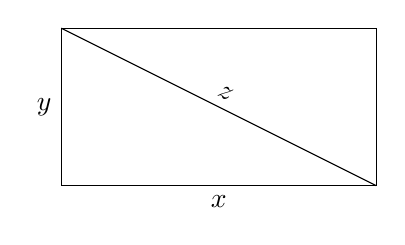
\begin{tikzpicture}
        \draw (0,0) rectangle (4,2);
        \draw (0,2) -- (4,0) node[pos=0.5,anchor=south,rotate=-26] {$z$};
        \node[anchor=east] at (0,1) {$y$};
        \node[anchor=north] at (2,0) {$x$};
    \end{tikzpicture}
    \end{center}
    At the instant when $x=4$ and $y=3$, what is the value of $\dfrac{\mathrm{d}x}{\mathrm{d}t}$?
    \begin{multicols}{3}
    \begin{choices}
        \wrongchoice{$\dfrac{1}{3}$}
      \correctchoice{$1$}
        \wrongchoice{$2$}
        \wrongchoice{$\sqrt{5}$}
        \wrongchoice{$5$}
    \end{choices}
    \end{multicols}
\end{question}
}

\element{calculusAB}{
\begin{questionmult}{1988-AB-q41}
    If $\lim_{x\to 3} f(x) = 7$, which of the following must be true?
    \begin{choices}
        %% ANS is A (sic)
        \wrongchoice{$f$ is continuous at $x=3$}
        \wrongchoice{$f$ is differentiable at $x=3$}
        \wrongchoice{$f(3) = 7$}
    \end{choices}
\end{questionmult}
}

\element{calculusAB}{
\begin{question}{1988-AB-q42}
    The graph of which of the following equations has $y=1$ as an asymptote?
    \begin{multicols}{2}
    \begin{choices}
        \wrongchoice{$y = \ln x$}
        \wrongchoice{$y = \sin x$}
      \correctchoice{$y = \dfrac{x}{x+1}$}
        \wrongchoice{$y = \dfrac{x^2}{x-1}$}
        \wrongchoice{$y = \mathrm{e}^{-x}$}
    \end{choices}
    \end{multicols}
\end{question}
}

\element{calculusAB}{
\begin{question}{1988-AB-q43}
    The volume of the solid obtained by revolving the region enclosed by the ellipse $x^2+9y^2=9$
        about the $x$-axis is
    \begin{multicols}{3}
    \begin{choices}
        \wrongchoice{$2\pi$}
      \correctchoice{$4\pi$}
        \wrongchoice{$6\pi$}
        \wrongchoice{$9\pi$}
        \wrongchoice{$12\pi$}
    \end{choices}
    \end{multicols}
\end{question}
}

\element{calculusAB}{
\begin{questionmult}{1988-AB-q44}
    Let $f$ and $g$ be odd functions.
    If $p$, $r$, and $s$ are nonzero functions defined as follows,
        which must be odd?
    \begin{choices}
        %% ANS is C
      \correctchoice{$p(x) = f\left(g(x)\right)$}
      \correctchoice{$r(x) = f(x) + g(x)$}
        \wrongchoice{$r(x) = f(x) g(x)$}
    \end{choices}
\end{questionmult}
}

\element{calculusAB}{
\begin{question}{1988-AB-q45}
    The volume of a cylindrical tin can with a top and a bottom is to be $16\pi$ cubic inches.
    If a minimum amount of tin is the be used to construct the can,
        what must be the height, in inches, of the can?
    \begin{multicols}{3}
    \begin{choices}
        \wrongchoice{$2 \sqrt[3]{2}$}
        \wrongchoice{$2 \sqrt{2}$}
        \wrongchoice{$2 \sqrt[3]{4}$}
      \correctchoice{$4$}
        \wrongchoice{$8$}
    \end{choices}
    \end{multicols}
\end{question}
}


%% 1993 AP Calculus AB: Section I (pp. 91)
%%--------------------------------------------------
\element{calculusAB}{
\begin{question}{1993-AB-q01}
    If $f(x) = x^{3/2}$, then $f\prime{}(4) = $
    \begin{multicols}{3}
    \begin{choices}
        \wrongchoice{$-6$}
        \wrongchoice{$-3$}
      \correctchoice{$3$}
        \wrongchoice{$6$}
        \wrongchoice{$8$}
    \end{choices}
    \end{multicols}
\end{question}
}

\element{calculusAB}{
\begin{question}{1993-AB-q02}
    Which of the following represents the area of the shaded region in the figure below?
    \begin{center}
    \begin{tikzpicture}
        \begin{axis}[
            axis y line=left,
            axis x line=bottom,
            axis line style={->},
            xlabel={$x$},
            xtick={1,5},
            xticklabels={$a$,$b$},
            x label style={
                at={(current axis.right of origin)},
                anchor=west,
            },
            ylabel={$y$},
            y label style={
                at={(current axis.above origin)},
                anchor=south,
                rotate=270,
            },
            ytick={1,2},
            yticklabels={$c$,$d$},
            xmin=0,xmax=5.5,
            ymin=0,ymax=2.2,
            width=0.8\columnwidth,
            height=0.5\columnwidth,
        ]
        \addplot[name path=A,line width=1pt,domain=1:5] {0.95833 + 0.04166 * x * x };
        \node[pin={290:$y=f(x)$}] at (3,1.33) {};
        \path[name path=B] (axis cs:1,2) -- (axis cs:5,2);
        \addplot[pattern=north west lines] fill between[of=A and B, soft clip={domain=1:5},];
        %% dashed lines
        \draw[dashed] (axis cs:1,0) -- (axis cs:1,2);
        \draw[dashed] (axis cs:5,0) -- (axis cs:5,2);
        \draw[dashed] (axis cs:0,2) -- (axis cs:5,2);
        \draw[dashed] (axis cs:0,1) -- (axis cs:1,1);
        \end{axis}
    \end{tikzpicture}
    \end{center}
    \begin{multicols}{2}
    \begin{choices}
        \wrongchoice{$\displaystyle \int^{\;\;d}_c f(y)\,\mathrm{d}y$}
      \correctchoice{$\displaystyle \int^{\;\;b}_a \left(d-f(x)\right)\,\mathrm{d}x$}
        \wrongchoice{$f\prime{}(b) - f\prime{}(a)$}
        \wrongchoice{$(b-a)\left[f(b) - f(a)\right]$}
        \wrongchoice{$(d-c)\left[f(b) - f(a)\right]$}
    \end{choices}
    \end{multicols}
\end{question}
}

\element{calculusAB}{
\begin{question}{1993-AB-q03}
    \begin{math}
        \displaystyle \lim_{n\to\infty} \dfrac{3n^3 - 5n}{n^3 - 2n^2+1}
    \end{math}
    is:
    \begin{multicols}{2}
    \begin{choices}
        \wrongchoice{$-5$}
        \wrongchoice{$-2$}
        \wrongchoice{$1$}
      \correctchoice{$3$}
        \wrongchoice{nonexistent}
    \end{choices}
    \end{multicols}
\end{question}
}

\element{calculusAB}{
\begin{question}{1993-AB-q04}
    If $x^3 + 3xy + 2y^3 = 17$, then in terms of $x$ and $y$,
        $\dfrac{\mathrm{d}y}{\mathrm{d}x} = $
    \begin{multicols}{2}
    \begin{choices}
      \correctchoice{$-\dfrac{x^2+y}{x+2y^2}$}
        \wrongchoice{$-\dfrac{x^2+y}{x+y^2}$}
        \wrongchoice{$-\dfrac{x^2+y}{x+2y}$}
        \wrongchoice{$-\dfrac{x^2+y}{2y^2}$}
        \wrongchoice{$-\dfrac{x^2}{1+2y^2}$}
    \end{choices}
    \end{multicols}
\end{question}
}

\element{calculusAB}{
\begin{question}{1993-AB-q05}
    If the function $f$ is continuous for all real numbers and if $f(x) = \dfrac{x^2-4}{x+2}$ when $x\neq -2$,
        then $f(-2) = $
    \begin{multicols}{3}
    \begin{choices}
      \correctchoice{$-4$}
        \wrongchoice{$-2$}
        \wrongchoice{$-1$}
        \wrongchoice{$0$}
        \wrongchoice{$2$}
    \end{choices}
    \end{multicols}
\end{question}
}

\element{calculusAB}{
\begin{question}{1993-AB-q06}
    The area of the region enclosed by the curve $y=\dfrac{1}{x-1}$,
        the $x$-axis, and the lines $x=3$ and $x=4$ is:
    \begin{multicols}{3}
    \begin{choices}
        \wrongchoice{$\dfrac{5}{36}$}
        \wrongchoice{$\ln\left(\dfrac{2}{3}\right)$}
        \wrongchoice{$\ln\left(\dfrac{4}{3}\right)$}
      \correctchoice{$\ln\left(\dfrac{3}{2}\right)$}
        \wrongchoice{$\ln\left(6\right)$}
    \end{choices}
    \end{multicols}
\end{question}
}

\element{calculusAB}{
\begin{question}{1993-AB-q07}
    An equation of the line tangent to the graph of $y=\dfrac{2x+3}{3x-2}$
        at the point $(1,5)$ is:
    \begin{multicols}{2}
    \begin{choices}
        \wrongchoice{$13 x - y = 8$}
      \correctchoice{$13 x + y = 18$}
        \wrongchoice{$x - 13 y = 64$}
        \wrongchoice{$x + 13 y = 66$}
        \wrongchoice{$-2 x + 3 y = 13$}
    \end{choices}
    \end{multicols}
\end{question}
}

\element{calculusAB}{
\begin{question}{1993-AB-q08}
    If $y=\tan x - \cot x$, then $\dfrac{\mathrm{d}y}{\mathrm{d}x}= $
    \begin{multicols}{2}
    \begin{choices}
        \wrongchoice{$\sec x \csc x$}
        \wrongchoice{$\sec x - \csc x$}
        \wrongchoice{$\sec x + \csc x$}
        \wrongchoice{$\sec^2 x - \csc^2 x$}
      \correctchoice{$\sec^2 x + \csc^2 x$}
    \end{choices}
    \end{multicols}
\end{question}
}

\element{calculusAB}{
\begin{question}{1993-AB-q09}
    If $h$ is the function given by $h(x) = f(g(x))$, where $f(x)=3x^2-1$
        and $g(x)=|x|$, then $h(x) = $
    \begin{multicols}{2}
    \begin{choices}
        \wrongchoice{$3 x^3 - |x|$}
        \wrongchoice{$|3 x^3 - 1|$}
        \wrongchoice{$3 x^2|x| - 1$}
        \wrongchoice{$3|x| - 1$}
      \correctchoice{$3x^2 - 1$}
    \end{choices}
    \end{multicols}
\end{question}
}

\element{calculusAB}{
\begin{question}{1993-AB-q10}
    If $f(x) = (x-1)^2 \sin x$, then  $f\prime{}(0) = $
    \begin{multicols}{3}
    \begin{choices}
        \wrongchoice{$-2$}
        \wrongchoice{$-1$}
        \wrongchoice{$0$}
      \correctchoice{$1$}
        \wrongchoice{$2$}
    \end{choices}
    \end{multicols}
\end{question}
}

\element{calculusAB}{
\begin{question}{1993-AB-q11}
    The acceleration of a particle moving along the $x$-axis at time $t$ is given by $a(t) = 6t-2$.
    If the velocity si 25 when $t=3$ and the position is 10 when $t=1$,
        then the position $x(t) = $
    \begin{multicols}{2}
    \begin{choices}
        \wrongchoice{$9t^2 + 1$}
        \wrongchoice{$3t^2 - 2t + 4$}
      \correctchoice{$t^3 - t^2 + 4t + 6$}
        \wrongchoice{$t^3 - t^2 + 9t + 20$}
        \wrongchoice{$36t^3 - 4t^2 + 77t + 55$}
    \end{choices}
    \end{multicols}
\end{question}
}

\element{calculusAB}{
\begin{questionmult}{1993-AB-q12}
    If $f$ and $g$ are continous functions,
        and if $f(x)\geq 0$ for all real numbers $x$,
        which of the following must be true?
    \begin{choices}
        \wrongchoice{$\displaystyle \int^{\;\;b}_a f(x) g(x) \mathrm{d}x = \left( \int^{\;\;b}_af(x) \mathrm{d}x\right)\left(\int^{\;\;b}_a g(x) \mathrm{d}x\right)$}
      \correctchoice{$\displaystyle \int^{\;\;b}_a\left(f(x)+g(x)\right) \mathrm{d}x = \int^{\;\;b}_af(x) \mathrm{d}x + \int^{\;\;b}_a g(x) \mathrm{d}x$}
        \wrongchoice{$\displaystyle \int^{\;\;b}_a\sqrt{f(x)} \mathrm{d}x = \sqrt{\int^{\;\;b}_a f(x)\mathrm{d}x}$}
    \end{choices}
\end{questionmult}
}

\element{calculusAB}{
\begin{question}{1993-AB-q13}
    The fundamental period of $2\cos\left(3x\right)$ is
    \begin{multicols}{3}
    \begin{choices}
      \correctchoice{$\dfrac{2\pi}{3}$}
        \wrongchoice{$2\pi$}
        \wrongchoice{$6\pi$}
        \wrongchoice{$2$}
        \wrongchoice{$3$}
    \end{choices}
    \end{multicols}
\end{question}
}

\element{calculusAB}{
\begin{question}{1993-AB-q14}
    $\displaystyle \int \dfrac{3x^2}{\sqrt{x^3+1}}\,\mathrm{d}x =$
    \begin{multicols}{2}
    \begin{choices}
      \correctchoice{$2\sqrt{x^3+1} + C$}
        \wrongchoice{$\dfrac{2}{3}\sqrt{x^3+1} + C$}
        \wrongchoice{$2\sqrt{x^3+1} + C$}
        \wrongchoice{$\ln\sqrt{x^3+1} + C$}
        \wrongchoice{$\ln\left(x^3+1\right) + C$}
    \end{choices}
    \end{multicols}
\end{question}
}

\element{calculusAB}{
\begin{question}{1993-AB-q15}
    For what value of $x$ does the function $f(x) = (x-2)(x-3)^2$ have a relative maximum?
    \begin{multicols}{3}
    \begin{choices}
        \wrongchoice{$-3$}
        \wrongchoice{$-\dfrac{7}{3}$}
        \wrongchoice{$-\dfrac{5}{2}$}
      \correctchoice{$\dfrac{7}{3}$}
        \wrongchoice{$\dfrac{5}{3}$}
    \end{choices}
    \end{multicols}
\end{question}
}

\element{calculusAB}{
\begin{question}{1993-AB-q16}
    The slope of the line \emph{normal} to the graph  of $y=2\ln\left(\sec x\right)$ at $x=\dfrac{\pi}{4}$ is:
    \begin{multicols}{2}
    \begin{choices}
        \wrongchoice{$-2$}
      \correctchoice{$-\dfrac{1}{2}$}
        \wrongchoice{$\dfrac{1}{2}$}
        \wrongchoice{$2$}
        \wrongchoice{nonexistent}
    \end{choices}
    \end{multicols}
\end{question}
}

\element{calculusAB}{
\begin{question}{1993-AB-q17}
    $\displaystyle\int\,\left(x^2+1\right)^2\,\mathrm{d}x=$
    \begin{multicols}{2}
    \begin{choices}
        \wrongchoice{$\dfrac{\left(x^2+1\right)^3}{3} + C$}
        \wrongchoice{$\dfrac{\left(x^2+1\right)^3}{6x} + C$}
        \wrongchoice{$\left(\dfrac{x^3}{3}+x\right)^2 + C$}
        \wrongchoice{$\dfrac{2x\left(x^2+1\right)^3}{3} + C$}
      \correctchoice{$\dfrac{x^5}{5} + \dfrac{2x^3}{3} + x + C$}
    \end{choices}
    \end{multicols}
\end{question}
}

\element{calculusAB}{
\begin{question}{1993-AB-q18}
    If $f(x)=\sin\left(\dfrac{x}{2}\right)$, then there exists a number $c$ in the interval $\dfrac{\pi}{2}<x<\dfrac{3\pi}{2}$ that satisfies the conclusion of the Mean Value Theorem.
    Which of the following could be $c$?
    \begin{multicols}{3}
    \begin{choices}
        \wrongchoice{$\dfrac{2\pi}{3}$}
        \wrongchoice{$\dfrac{3\pi}{4}$}
        \wrongchoice{$\dfrac{5\pi}{6}$}
      \correctchoice{$\pi$}
        \wrongchoice{$\dfrac{3\pi}{2}$}
    \end{choices}
    \end{multicols}
\end{question}
}

\element{calculusAB}{
\begin{question}{1993-AB-q19}
    Let $f$ be the function defined by
    \begin{equation*}
        f(x) = 
        \begin{cases}
            x^3 & \text{for } x\leq 0, \\
            x   & \text{for } x> 0. \\
        \end{cases}
    \end{equation*}
    Which of the following statements about $f$ is true?
    \begin{choices}
        \wrongchoice{$f$ is an odd function}
        \wrongchoice{$f$ is discontinuous at $x=0$}
        \wrongchoice{$f$ has a relative maximum}
        \wrongchoice{$f^\prime{}(0) = 0$}
      \correctchoice{$f^\prime{}(x)>0$ for $x\neq 0$}
    \end{choices}
\end{question}
}

\element{calculusAB}{
\begin{question}{1993-AB-q20}
    Let $R$ be the region in the first quadrant enclosed by the graph of $y=(x+1)^{1/3}$,
        the line $x=7$, the $x$-axis, and the $y$-axis.
    The volume of the solid generated when $R$ is revolved about the $y$-axis is given by:
    \begin{multicols}{2}
    \begin{choices}
        \wrongchoice{$\displaystyle\pi\int^{\;\;7}_0\,\left(x+1\right)^{2/3}\,\mathrm{d}x$}
      \correctchoice{$\displaystyle{}2\pi\int^{\;\;7}_0\,x\left(x+1\right)^{1/3}\,\mathrm{d}x$}
        \wrongchoice{$\displaystyle\pi\int^{\;\;2}_0\,\left(x+1\right)^{2/3}\,\mathrm{d}x$}
        \wrongchoice{$\displaystyle{}2\pi\int^{\;\;2}_0\,x\left(x+1\right)^{1/3}\,\mathrm{d}x$}
        \wrongchoice{$\displaystyle\pi\int^{\;\;7}_0\,x\left(y^3-1\right)^{2}\,\mathrm{d}y$}
    \end{choices}
    \end{multicols}
\end{question}
}

\element{calculusAB}{
\begin{question}{1993-AB-q21}
    At what value of $x$ does the graph of $y=\dfrac{1}{x^2}-\dfrac{1}{x^3}$ have a point of inflection?
    \begin{multicols}{2}
    \begin{choices}
        \wrongchoice{$0$}
        \wrongchoice{$1$}
      \correctchoice{$2$}
        \wrongchoice{$3$}
        \wrongchoice{At  no value of $x$}
    \end{choices}
    \end{multicols}
\end{question}
}

\element{calculusAB}{
\begin{question}{1993-AB-q22}
    An antiderivative for $\dfrac{1}{x^2-2x+2}$ is
    \begin{multicols}{2}
    \begin{choices}
        \wrongchoice{$-\left(x^2-2x+2\right)^{-2}$}
        \wrongchoice{$\ln\left(x^2-2x+2\right)$}
        \wrongchoice{$\ln\left|\dfrac{x-2}{x+1}\right|$}
        \wrongchoice{$\mathrm{arcsec}\left(x-1\right)$}
      \correctchoice{$\mathrm{arctan}\left(x-1\right)$}
    \end{choices}
    \end{multicols}
\end{question}
}

\element{calculusAB}{
\begin{question}{1993-AB-q23}
    How many critical points does the function $f(x)=(x+2)^5(x-3)^4$ have?
    \begin{multicols}{3}
    \begin{choices}
        \wrongchoice{one}
        \wrongchoice{two}
      \correctchoice{three}
        \wrongchoice{five}
        \wrongchoice{nine}
    \end{choices}
    \end{multicols}
\end{question}
}

\element{calculusAB}{
\begin{question}{1993-AB-q24}
    If $f(x) = (x^2-2x-1)^{2/3}$, then $f\prime{}(0)$ is:
    \begin{multicols}{3}
    \begin{choices}
      \correctchoice{$\dfrac{4}{3}$}
        \wrongchoice{zero}
        \wrongchoice{$-\dfrac{2}{3}$}
        \wrongchoice{$-\dfrac{4}{3}$}
        \wrongchoice{$-2$}
    \end{choices}
    \end{multicols}
\end{question}
}

\element{calculusAB}{
\begin{question}{1993-AB-q25}
    $\displaystyle \frac{\mathrm{d}}{\mathrm{d}x}\left(2^x\right) = $
    \begin{multicols}{2}
    \begin{choices}
        \wrongchoice{$2^{x-1}$}
        \wrongchoice{$\left(2^{x-1}\right)x$}
      \correctchoice{$\left(2^{x}\right)\ln 2$}
        \wrongchoice{$\left(2^{x-1}\right)\ln 2$}
        \wrongchoice{$\dfrac{2x}{\ln 2}$}
    \end{choices}
    \end{multicols}
\end{question}
}

\element{calculusAB}{
\begin{question}{1993-AB-q26}
    A particle moves along a line so that at time $t$, where $0\leq t\leq \pi$,
        its position is given by $s(t) = -4\cos t - \frac{t^2}{2} + 10$.
    What is the velocity of the particle when its acceleration is zero?
    \begin{multicols}{2}
    \begin{choices}
        \wrongchoice{$-5.19$}
        \wrongchoice{$0.74$}
        \wrongchoice{$1.32$}
      \correctchoice{$2.55$}
        \wrongchoice{$8.13$}
    \end{choices}
    \end{multicols}
\end{question}
}

\element{calculusAB}{
\begin{question}{1993-AB-q27}
    The function $f$ given by $f(x) = x^3 + 12x - 24$ is:
    \begin{choices}
        \wrongchoice{increasing for $x<-2$, decreasing for $-2<x<2$, increasing for $x>2$}
        \wrongchoice{decreasing for $x<0$, increasing for $x>0$}
      \correctchoice{increasing for all $x$}
        \wrongchoice{decreasing for all $x$}
        \wrongchoice{decreasing for $x<-2$, increasing for $-2<x<2$, decreasing for $x>2$}
    \end{choices}
\end{question}
}

\element{calculusAB}{
\begin{question}{1993-AB-q28}
    $\displaystyle \int^{\;\;500}_1\,\left(13^x - 11^x\right)\,\mathrm{d}x + \int^{\;\;500}_2\,\left(11^2-13^x\right)\,\mathrm{d}x = $
    \begin{multicols}{2}
    \begin{choices}
        \wrongchoice{0.000}
      \correctchoice{14.946}
        \wrongchoice{34.415}
        \wrongchoice{46.000}
        \wrongchoice{136.364}
    \end{choices}
    \end{multicols}
\end{question}
}

\element{calculusAB}{
\begin{question}{1993-AB-q29}
    $\displaystyle \lim_{\theta\to 0} \dfrac{1-\cos\theta}{2\sin^2\theta} =$
    \begin{multicols}{2}
    \begin{choices}
        \wrongchoice{zero}
        \wrongchoice{$\dfrac{1}{8}$}
      \correctchoice{$\dfrac{1}{4}$}
        \wrongchoice{one}
        \wrongchoice{nonexistent}
    \end{choices}
    \end{multicols}
\end{question}
}

\element{calculusAB}{
\begin{question}{1993-AB-q30}
    The region enclosed by the $x$-axis, the line $x=3$,
        and the curve $y=\sqrt{x}$ is rotated about the $x$-axis.
    What is the volume of the solid generated?
    \begin{multicols}{3}
    \begin{choices}
        \wrongchoice{$3\pi$}
        \wrongchoice{$2\sqrt{3}\pi$}
      \correctchoice{$\dfrac{9}{2}\pi$}
        \wrongchoice{$9\pi$}
        \wrongchoice{$\dfrac{36\sqrt{3}}{5}\pi$}
    \end{choices}
    \end{multicols}
\end{question}
}

\element{calculusAB}{
\begin{question}{1993-AB-q31}
    If $f(x) = \mathrm{e}^{3\ln x^2}$, then $f\prime{}(x) = $
    \begin{multicols}{2}
    \begin{choices}
        \wrongchoice{$\mathrm{e}^{3\ln x^2}$}
        \wrongchoice{$\dfrac{3}{x^2}\mathrm{e}^{3\ln x^2}$}
        \wrongchoice{$6\left(\ln x\right)\mathrm{e}^{3\ln x^2}$}
        \wrongchoice{$5x^4$}
      \correctchoice{$6x^5$}
    \end{choices}
    \end{multicols}
\end{question}
}

\element{calculusAB}{
\begin{question}{1993-AB-q32}
    $\displaystyle \int^{\;\;\sqrt{3}}_0\,\dfrac{\mathrm{d}x}{\sqrt{4-x^2}} =$
    \begin{multicols}{2}
    \begin{choices}
      \correctchoice{$\dfrac{\pi}{3}$}
        \wrongchoice{$\dfrac{\pi}{4}$}
        \wrongchoice{$\dfrac{\pi}{6}$}
        \wrongchoice{$\dfrac{1}{2}\ln 2$}
        \wrongchoice{$-\ln 2$}
    \end{choices}
    \end{multicols}
\end{question}
}

\element{calculusAB}{
\begin{question}{1993-AB-q33}
    If $\dfrac{\mathrm{d}y}{\mathrm{d}x} = 2y^2$ and if $y=-1$ when $x=1$,
        then when $x=2$, $y=$
    \begin{multicols}{2}
    \begin{choices}
        \wrongchoice{$-\dfrac{2}{3}$}
      \correctchoice{$-\dfrac{1}{3}$}
        \wrongchoice{zero}
        \wrongchoice{$\dfrac{1}{3}$}
        \wrongchoice{$\dfrac{2}{3}$}
    \end{choices}
    \end{multicols}
\end{question}
}

\element{calculusAB}{
\begin{question}{1993-AB-q34}
    The top of a 25 foot ladder is sliding down a vertical wall at a constant rate of 3 feet per minute.
    When the top of the ladder is 7 feet from the ground,
        what is the rate of change of the distance between the bottom of the ladder and the wall?
    \begin{choices}
        \wrongchoice{$-\dfrac{7}{8}$ feet per minute}
        \wrongchoice{$-\dfrac{7}{24}$ feet per minute}
        \wrongchoice{$\dfrac{7}{24}$ feet per minute}
      \correctchoice{$\dfrac{7}{8}$ feet per minute}
        \wrongchoice{$\dfrac{21}{25}$ feet per minute}
    \end{choices}
\end{question}
}

\element{calculusAB}{
\begin{question}{1993-AB-q35}
    If the graph of $y=\dfrac{ax+b}{x+c}$ has a horizontal asymptote $y=2$ and a vertical asymptote $x=-3$,
        then $a+c=$
    \begin{multicols}{3}
    \begin{choices}
        \wrongchoice{$-5$}
        \wrongchoice{$-1$}
        \wrongchoice{Zero}
        \wrongchoice{$1$}
      \correctchoice{$5$}
    \end{choices}
    \end{multicols}
\end{question}
}

\element{calculusAB}{
\begin{question}{1993-AB-q36}
    If the definite integral $\int^{\,\,2}_0 \mathrm{e}^{x^2}\,\mathrm{d}x$ is first approximated by using two \emph{inscribed} rectangles of equal width and then approximated by using the trapezoidal rule with $n=2$,
        the difference between the two approximations is:
    \begin{multicols}{2}
    \begin{choices}
        \wrongchoice{$53.60$}
        \wrongchoice{$30.51$}
        \wrongchoice{$27.80$}
      \correctchoice{$26.80$}
        \wrongchoice{$12.78$}
    \end{choices}
    \end{multicols}
\end{question}
}

\element{calculusAB}{
\begin{question}{1993-AB-q37}
    If $f$ is a differentiable function,
        then $f\prime{}(a)$ is given by which of the following?
    \begin{itemize}
        \item[I.]   $\displaystyle \lim_{h\to 0} \dfrac{f(a+h) - f(a)}{h}$
        \item[II.]  $\displaystyle \lim_{h\to a} \dfrac{f(x) - f(a)}{x-a}$
        \item[III.] $\displaystyle \lim_{h\to a} \dfrac{f(x+h) - f(x)}{h}$
    \end{itemize}
    \begin{multicols}{2}
    \begin{choices}
        \wrongchoice{I only}
        \wrongchoice{II only}
      \correctchoice{I and II only}
        \wrongchoice{I and III only}
        \wrongchoice{I, II and III}
    \end{choices}
    \end{multicols}
\end{question}
}

\element{calculusAB}{
\begin{question}{1993-AB-q38}
    If the second derivative of $f$ is given by $f\dprime{}(x) = 2x-\cos x$,
        which of the following could be $f(x)$?
    \begin{multicols}{2}
    \begin{choices}
      \correctchoice{$\dfrac{x^3}{3} + \cos x - x + 1$}
        \wrongchoice{$\dfrac{x^3}{3} + \cos x - x + 1$}
        \wrongchoice{$x^3 + \cos x - x + 1$}
        \wrongchoice{$x^3 - \sin x + 1$}
        \wrongchoice{$x^3 + \sin x + 1$}
    \end{choices}
    \end{multicols}
\end{question}
}

\element{calculusAB}{
\begin{question}{1993-AB-q39}
    The radius of a circle is increasing at a nonzero rate,
        and at a certain instant,
        the rate of increase in the area of the circle is numerically equal to the rate of increase in its circumference.
    At this instant,
        the radius of the circle is:
    \begin{multicols}{3}
    \begin{choices}
        \wrongchoice{$\dfrac{1}{\pi}$}
        \wrongchoice{$\dfrac{1}{2}$}
        \wrongchoice{$\dfrac{2}{\pi}$}
      \correctchoice{$1$}
        \wrongchoice{$2$}
    \end{choices}
    \end{multicols}
\end{question}
}

\element{calculusAB}{
\begin{question}{1993-AB-q40}
    The grpah of $y=f(x)$ is shown in the figure below.
    \begin{center}
    \begin{tikzpicture}
        \begin{axis}[
            axis y line=middle,
            axis x line=middle,
            axis line style={->},
            xlabel={$x$},
            xtick={-4,-1,1,4},
            x label style={
                at={(current axis.right of origin)},
                anchor=west,
            },
            ylabel={$y$},
            y label style={
                at={(current axis.above origin)},
                anchor=south,
            },
            ytick=\empty,
            xmin=-4.5,xmax=4.5,
            ymin=-4,ymax=4,
            width=0.8\columnwidth,
            height=0.5\columnwidth,
            very thin,
        ]
        \addplot[line width=1pt,domain=-4:4] {0.2 * (x+4) * (x+1) * (x-1)};
        \end{axis}
    \end{tikzpicture}
    \end{center}
    Which of the following could be the graph $y=f\left(\left|x\right|\right)$?
    \begin{multicols}{2}
    \begin{choices}
        \AMCboxDimensions{down=-2.5em}
        \wrongchoice{
            \begin{tikzpicture}
                \begin{axis}[
                    axis y line=middle,
                    axis x line=middle,
                    axis line style={->},
                    xlabel={$x$},
                    xtick={-4,-1,1,4},
                    x label style={
                        at={(current axis.right of origin)},
                        anchor=west,
                    },
                    ylabel={$y$},
                    y label style={
                        at={(current axis.above origin)},
                        anchor=south,
                    },
                    ytick=\empty,
                    xmin=-4.5,xmax=4.5,
                    ymin=-4,ymax=4,
                    width=0.95\columnwidth,
                    very thin,
                ]
                \addplot[line width=1pt,domain=-4:4] {0.2 * (x+4) * (x+1) * (x-1)};
                \end{axis}
            \end{tikzpicture}
        }
        \wrongchoice{
            \begin{tikzpicture}
                \begin{axis}[
                    axis y line=middle,
                    axis x line=middle,
                    axis line style={->},
                    xlabel={$x$},
                    xtick={-4,-1,1,4},
                    x label style={
                        at={(current axis.right of origin)},
                        anchor=west,
                    },
                    ylabel={$y$},
                    y label style={
                        at={(current axis.above origin)},
                        anchor=south,
                    },
                    ytick=\empty,
                    xmin=-4.5,xmax=4.5,
                    ymin=-4,ymax=4,
                    width=0.95\columnwidth,
                    very thin,
                ]
                \addplot[line width=1pt,domain=0:4] {abs(0.2 * (x+4) * (x+1) * (x-1))};
                \end{axis}
            \end{tikzpicture}
        }
        %% ANS is C
        \correctchoice{
            \begin{tikzpicture}
                \begin{axis}[
                    axis y line=middle,
                    axis x line=middle,
                    axis line style={->},
                    xlabel={$x$},
                    xtick={-4,-1,1,4},
                    x label style={
                        at={(current axis.right of origin)},
                        anchor=west,
                    },
                    ylabel={$y$},
                    y label style={
                        at={(current axis.above origin)},
                        anchor=south,
                    },
                    ytick=\empty,
                    xmin=-4.5,xmax=4.5,
                    ymin=-4,ymax=4,
                    width=0.95\columnwidth,
                    very thin,
                ]
                \addplot[line width=1pt,domain=-4:4] {0.2 * (abs(x)+4) * (abs(x)+1) * (abs(x)-1)};
                \end{axis}
            \end{tikzpicture}
        }
        \wrongchoice{
            \begin{tikzpicture}
                \begin{axis}[
                    axis y line=middle,
                    axis x line=middle,
                    axis line style={->},
                    xlabel={$x$},
                    xtick={-4,-1,1,4},
                    x label style={
                        at={(current axis.right of origin)},
                        anchor=west,
                    },
                    ylabel={$y$},
                    y label style={
                        at={(current axis.above origin)},
                        anchor=south,
                    },
                    ytick=\empty,
                    xmin=-4.5,xmax=4.5,
                    ymin=-4,ymax=4,
                    width=0.95\columnwidth,
                    very thin,
                ]
                \addplot[line width=1pt,domain=-4:4] {abs(0.2 * (x+4) * (x+1) * (x-1))};
                \end{axis}
            \end{tikzpicture}
        }
        \wrongchoice{
            \begin{tikzpicture}
                \begin{axis}[
                    axis y line=middle,
                    axis x line=middle,
                    axis line style={->},
                    xlabel={$x$},
                    xtick={-4,-1,1,4},
                    x label style={
                        at={(current axis.right of origin)},
                        anchor=west,
                    },
                    ylabel={$y$},
                    y label style={
                        at={(current axis.above origin)},
                        anchor=south,
                    },
                    ytick=\empty,
                    xmin=-4.5,xmax=4.5,
                    ymin=-4,ymax=4,
                    width=0.95\columnwidth,
                    very thin,
                ]
                \addplot[line width=1pt,domain=-4:4] {abs( 0.2 * (abs(x)+4) * (abs(x)+1) * (abs(x)-1) )};
                \end{axis}
            \end{tikzpicture}
        }
    \end{choices}
    \end{multicols}
\end{question}
}

\element{calculusAB}{
\begin{question}{1993-AB-q41}
    $\displaystyle \frac{\mathrm{d}}{\mathrm{d}x}\int^{\;\;x}_0 \cos\left(2\pi u\right)\,\mathrm{d}u =$
    \begin{multicols}{2}
    \begin{choices}
        \wrongchoice{$0$}
        \wrongchoice{$\dfrac{1}{2\pi}\sin x$}
        \wrongchoice{$\dfrac{1}{2\pi}\cos\left(2\pi x\right)$}
      \correctchoice{$\cos\left(2\pi x\right)$}
        \wrongchoice{$2\pi\cos\left(2\pi x\right)$}
    \end{choices}
    \end{multicols}
\end{question}
}

\element{calculusAB}{
\begin{question}{1993-AB-q42}
    A puppy weighs 2.0 pounds at birth and 3.5 pounds two months later.
    If the weight of the puppy during its first 6 months is increasing at a rate proportional to its weight,
        then how much will the puppy weigh when it is three months old?
    \begin{multicols}{2}
    \begin{choices}
        \wrongchoice{4.2 pounds}
      \correctchoice{4.6 pounds}
        \wrongchoice{4.8 pounds}
        \wrongchoice{5.6 pounds}
        \wrongchoice{6.5 pounds}
    \end{choices}
    \end{multicols}
\end{question}
}

\element{calculusAB}{
\begin{question}{1993-AB-q43}
    $\displaystyle \int\,xf(x)\,\mathrm{d}x = $
    \begin{multicols}{2}
    \begin{choices}
        \wrongchoice{$xf(x) - \int,xf\prime{}(x)\,\mathrm{d}x$}
      \correctchoice{$\dfrac{x^2}{2} f(x) - \int\dfrac{x^2}{x}f\prime{}(x)\,\mathrm{d}x$}
        \wrongchoice{$xf(x) - \dfrac{x^2}{2}f(x) + C$}
        \wrongchoice{$xf(x) - \int f\prime{}(x)\,\mathrm{d}x$}
        \wrongchoice{$\dfrac{x^2}{2} \int f(x)\,\mathrm{d}x$}
    \end{choices}
    \end{multicols}
\end{question}
}

\element{calculusAB}{
\begin{question}{1993-AB-q44}
    What is the minimum value of $f(x) = x\ln x$?
    \begin{choices}
        \wrongchoice{$-\mathrm{e}$}
        \wrongchoice{$-1$}
      \correctchoice{$-\dfrac{1}{\mathrm{e}}$}
        \wrongchoice{$0$}
        \wrongchoice{$f(x)$ has no minimum value.}
    \end{choices}
\end{question}
}

\element{calculusAB}{
\begin{question}{1993-AB-q45}
    If Newton's method is used to approximate the real root of $x^3 + x - 1 = 0$,
        then a first approximation $x_1 = 1$ would lead to a \emph{third} approximation of $x_3=$
    \begin{multicols}{3}
    \begin{choices}
        \wrongchoice{0.682}
      \correctchoice{0.686}
        \wrongchoice{0.694}
        \wrongchoice{0.750}
        \wrongchoice{1.637}
    \end{choices}
    \end{multicols}
\end{question}
}


%% 1997 AP Calculus AB: Section I (pp. 106)
%%--------------------------------------------------
\element{calculusAB}{
\begin{question}{1997-AB-q01}
    $\displaystyle \int^{\;\;2}_1 \left(4x^3 - 6x\right)\,\mathrm{d}x = $
    \begin{multicols}{3}
    \begin{choices}
        \wrongchoice{2}
        \wrongchoice{4}
      \correctchoice{6}
        \wrongchoice{36}
        \wrongchoice{42}
    \end{choices}
    \end{multicols}
\end{question}
}

\element{calculusAB}{
\begin{question}{1997-AB-q02}
    If $f(x) = x \sqrt{2x-3}$,
        then $f\prime{}(x) = $
    \begin{multicols}{2}
    \begin{choices}
      \correctchoice{$\dfrac{3x-3}{\sqrt{2x-3}}$}
        \wrongchoice{$\dfrac{x}{\sqrt{2x-3}}$}
        \wrongchoice{$\dfrac{1}{\sqrt{2x-3}}$}
        \wrongchoice{$\dfrac{-x+3}{\sqrt{2x-3}}$}
        \wrongchoice{$\dfrac{5x-6}{2\sqrt{2x-3}}$}
    \end{choices}
    \end{multicols}
\end{question}
}

\element{calculusAB}{
\begin{question}{1997-AB-q03}
    If $\int^{\,\,b}_a f(x)\,\mathrm{d}x = a+2b$,
        then $\int^{\,\,b}_a\left(f(x)+5\right)\,\mathrm{d}x = $
    \begin{multicols}{2}
    \begin{choices}
        \wrongchoice{$a + 2b + 5$}
        \wrongchoice{$5b - 5a$}
      \correctchoice{$7b - 4a$}
        \wrongchoice{$7b - 5a$}
        \wrongchoice{$7b - 6a$}
    \end{choices}
    \end{multicols}
\end{question}
}

\element{calculusAB}{
\begin{question}{1997-AB-q04}
    If $f(x) = -x^3 + x + \dfrac{1}{x}$,
        then $f\prime{}\left(-1\right) = $
    \begin{multicols}{3}
    \begin{choices}
        \wrongchoice{$3$}
        \wrongchoice{$1$}
        \wrongchoice{$-1$}
      \correctchoice{$-3$}
        \wrongchoice{$-5$}
    \end{choices}
    \end{multicols}
\end{question}
}

\element{calculusAB}{
\begin{question}{1997-AB-q05}
    The graph of $y= 3x^4 - 16x^3 + 24 x^2 + 48$ is concave down for:
    \begin{multicols}{2}
    \begin{choices}
        \wrongchoice{$x < 0$}
        \wrongchoice{$x > 0$}
        \wrongchoice{$x < -2$ or $x > -\dfrac{2}{3}$}
        \wrongchoice{$x < \dfrac{2}{3}$ or $x > 2$}
      \correctchoice{$\dfrac{2}{3} < x < 2$}
    \end{choices}
    \end{multicols}
\end{question}
}

\element{calculusAB}{
\begin{question}{1997-AB-q06}
    $\displaystyle \dfrac{1}{2} \int\mathrm{e}^{\tfrac{t}{2}}\,\mathrm{d}t =$
    \begin{multicols}{2}
    \begin{choices}
        \wrongchoice{$\mathrm{e}^{-t} + C$}
        \wrongchoice{$\mathrm{e}^{-\tfrac{t}{2}} + C$}
      \correctchoice{$\mathrm{e}^{\tfrac{t}{2}} + C$}
        \wrongchoice{$2\mathrm{e}^{\tfrac{t}{2}} + C$}
        \wrongchoice{$\mathrm{e}^{t} + C$}
    \end{choices}
    \end{multicols}
\end{question}
}

\element{calculusAB}{
\begin{question}{1997-AB-q07}
    $\displaystyle \dfrac{\mathrm{d}}{\mathrm{d}x} \cos^2\left(x^3\right) = $
    \begin{multicols}{2}
    \begin{choices}
        \wrongchoice{$6x^2 \sin\left(x^3\right)\cos\left(x^3\right)$}
        \wrongchoice{$6x^2 \cos\left(x^3\right)$}
        \wrongchoice{$\sin^2\left(x^3\right)$}
      \correctchoice{$-6x^2 \sin\left(x^3\right)\cos\left(x^3\right)$}
        \wrongchoice{$-2 \sin\left(x^3\right)\cos\left(x^3\right)$}
    \end{choices}
    \end{multicols}
\end{question}
}

\newcommand{\calculusABNinetySevenQEight}{
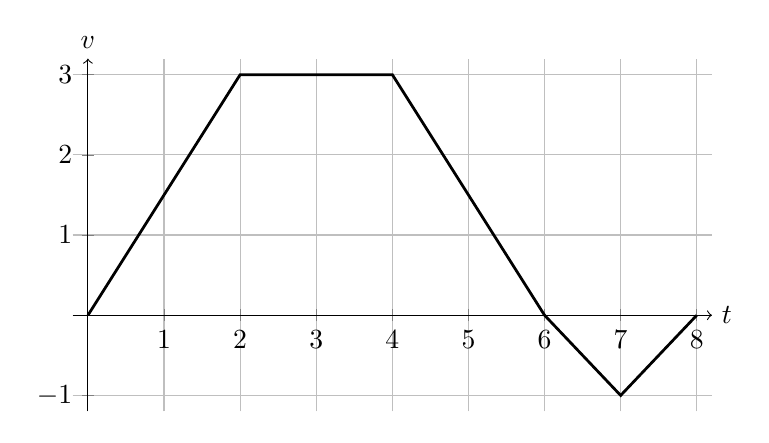
\begin{tikzpicture}
    \begin{axis}[
        axis y line=middle,
        axis x line=middle,
        axis line style={->},
        xlabel={$t$},
        xtick={0,1,2,3,4,5,6,7,8},
        x label style={
            at={(current axis.right of origin)},
            anchor=west,
        },
        ylabel={$v$},
        y label style={
            at={(current axis.above origin)},
            anchor=south,
        },
        ytick={-1,0,1,2,3},
        xmin=-0.2,xmax=8.2,
        ymin=-1.2,ymax=3.2,
        grid=major,
        width=0.8\columnwidth,
        height=0.5\columnwidth,
    ]
    \addplot[line width=1pt,mark=\empty] plot coordinates {(0,0) (2,3) (4,3) (6,0) (7,-1) (8,0)};
    \end{axis}
\end{tikzpicture}
}

\element{calculusAB}{
\begin{question}{1997-AB-q08}
    A bug begins to crawl up a vertical wire at time $t=0$.
    The velocity $v$ of the bug at time $t$,
        $0 \leq t \leq 8$, is given by the function whose graph is shown below.
    \begin{center}
        \calculusABNinetySevenQEight
    \end{center}
    At what value of $t$ does the bug change direction?
    \begin{multicols}{3}
    \begin{choices}
        \wrongchoice{2}
        \wrongchoice{4}
      \correctchoice{6}
        \wrongchoice{7}
        \wrongchoice{8}
    \end{choices}
    \end{multicols}
\end{question}
}

\element{calculusAB}{
\begin{question}{1997-AB-q09}
    A bug begins to crawl up a vertical wire at time $t=0$.
    The velocity $v$ of the bug at time $t$,
        $0 \leq t \leq 8$, is given by the function whose graph is shown below.
    \begin{center}
        \calculusABNinetySevenQEight
    \end{center}
    What is the total distance the bug traveled from $t=0$ to $t=8$
    \begin{multicols}{3}
    \begin{choices}
        \wrongchoice{$14$}
      \correctchoice{$13$}
        \wrongchoice{$11$}
        \wrongchoice{$8$}
        \wrongchoice{$6$}
    \end{choices}
    \end{multicols}
\end{question}
}

\element{calculusAB}{
\begin{question}{1997-AB-q10}
    An equation of the line tangent to the graph of $y=\cos\left(2x\right)$ at $x=\dfrac{\pi}{4}$ is:
    \begin{multicols}{2}
    \begin{choices}
        \wrongchoice{$y-1 = -\left(x-\dfrac{\pi}{4}\right)$}
        \wrongchoice{$y-1 = -2\left(x-\dfrac{\pi}{4}\right)$}
        \wrongchoice{$y = 2\left(x-\dfrac{\pi}{4}\right)$}
        \wrongchoice{$y = -\left(x-\dfrac{\pi}{4}\right)$}
      \correctchoice{$y = -2\left(x-\dfrac{\pi}{4}\right)$}
    \end{choices}
    \end{multicols}
\end{question}
}

\element{calculusAB}{
\begin{question}{1997-AB-q11}
    The graph of the derivative of $f$ is shown in the figure below.
    \begin{center}
    \begin{tikzpicture}
        \begin{axis}[
            axis y line=middle,
            axis x line=middle,
            axis line style={->},
            xlabel={$x$},
            xtick={-2,0,2},
            x label style={
                at={(current axis.right of origin)},
                anchor=west,
            },
            ylabel={$y$},
            y label style={
                at={(current axis.above origin)},
                anchor=south,
            },
            ytick=\empty,
            xmin=-3,xmax=3,
            ymin=-3,ymax=3,
            width=0.8\columnwidth,
            height=0.5\columnwidth,
            clip=false,
        ]
        \addplot[line width=1pt,domain=-3:3] {-0.666 * (x+2) * (x-2)};
        \node[pin={[pin edge=latex-]60:$y=f\prime{}(x)$}] at (axis cs:1,2) {};
        \end{axis}
    \end{tikzpicture}
    \end{center}
    Which of the following could be the graph of $f\prime{}$?
    \begin{multicols}{2}
    \begin{choices}
        \AMCboxDimensions{down=-2.5em}
        \wrongchoice{
            \begin{tikzpicture}
                \begin{axis}[
                    axis y line=middle,
                    axis x line=middle,
                    axis line style={->},
                    xlabel={$x$},
                    xtick={-2,0,2},
                    x label style={
                        at={(current axis.right of origin)},
                        anchor=west,
                    },
                    ylabel={$y$},
                    y label style={
                        at={(current axis.above origin)},
                        anchor=south,
                    },
                    ytick=\empty,
                    xmin=-3,xmax=3,
                    ymin=-3,ymax=3,
                    width=0.95\columnwidth,
                ]
                \addplot[line width=1pt,domain=-3:3] {x};
                \end{axis}
            \end{tikzpicture}
        }
        \wrongchoice{
            \begin{tikzpicture}
                \begin{axis}[
                    axis y line=middle,
                    axis x line=middle,
                    axis line style={->},
                    xlabel={$x$},
                    xtick={-2,0,2},
                    x label style={
                        at={(current axis.right of origin)},
                        anchor=west,
                    },
                    ylabel={$y$},
                    y label style={
                        at={(current axis.above origin)},
                        anchor=south,
                    },
                    ytick=\empty,
                    xmin=-3,xmax=3,
                    ymin=-3,ymax=3,
                    width=0.95\columnwidth,
                ]
                \addplot[line width=1pt,domain=-3:3] {-x};
                \end{axis}
            \end{tikzpicture}
        }
        \wrongchoice{
            \begin{tikzpicture}
                \begin{axis}[
                    axis y line=middle,
                    axis x line=middle,
                    axis line style={->},
                    xlabel={$x$},
                    xtick={-2,0,2},
                    x label style={
                        at={(current axis.right of origin)},
                        anchor=west,
                    },
                    ylabel={$y$},
                    y label style={
                        at={(current axis.above origin)},
                        anchor=south,
                    },
                    ytick=\empty,
                    xmin=-3,xmax=3,
                    ymin=-3,ymax=3,
                    width=0.95\columnwidth,
                ]
                \addplot[line width=1pt,domain=-3:3] {0.66 * x * (x+2) * (x-2)};
                \end{axis}
            \end{tikzpicture}
        }
        \wrongchoice{
            \begin{tikzpicture}
                \begin{axis}[
                    axis y line=middle,
                    axis x line=middle,
                    axis line style={->},
                    xlabel={$x$},
                    xtick={-2,0,2},
                    x label style={
                        at={(current axis.right of origin)},
                        anchor=west,
                    },
                    ylabel={$y$},
                    y label style={
                        at={(current axis.above origin)},
                        anchor=south,
                    },
                    ytick=\empty,
                    xmin=-3,xmax=3,
                    ymin=-3,ymax=3,
                    width=0.95\columnwidth,
                ]
                \addplot[line width=1pt,domain=-3:3] {0.15 * (x^3 - 12*x)};
                \end{axis}
            \end{tikzpicture}
        }
        %% ANS is E
        \correctchoice{
            \begin{tikzpicture}
                \begin{axis}[
                    axis y line=middle,
                    axis x line=middle,
                    axis line style={->},
                    xlabel={$x$},
                    xtick={-2,0,2},
                    x label style={
                        at={(current axis.right of origin)},
                        anchor=west,
                    },
                    ylabel={$y$},
                    y label style={
                        at={(current axis.above origin)},
                        anchor=south,
                    },
                    ytick=\empty,
                    xmin=-3,xmax=3,
                    ymin=-3,ymax=3,
                    width=0.95\columnwidth,
                ]
                \addplot[line width=1pt,domain=-3:3] {-0.15 * (x^3 - 12*x)};
                \end{axis}
            \end{tikzpicture}
        }
    \end{choices}
    \end{multicols}
\end{question}
}

\element{calculusAB}{
\begin{question}{1997-AB-q12}
    At what point on the graph of $y=\dfrac{1}{2} x^2$ is the tangent line parallel to the line $2x - 4y = 3$?
    \begin{multicols}{2}
    \begin{choices}
        \wrongchoice{$\left(\dfrac{1}{2},-\dfrac{1}{2}\right)$}
      \correctchoice{$\left(\dfrac{1}{2},\dfrac{1}{8}\right)$}
        \wrongchoice{$\left(1,-\dfrac{1}{4}\right)$}
        \wrongchoice{$\left(1,\dfrac{1}{2}\right)$}
        \wrongchoice{$\left(2,2\right)$}
    \end{choices}
    \end{multicols}
\end{question}
}

\element{calculusAB}{
\begin{question}{1997-AB-q13}
    Let $f$ be a function defined for all real numbers $x$.
    If $f\prime{}(x) = \dfrac{\left|4-x^2\right|}{x-2}$,
        then $f$ is decreasing on the interval:
    \begin{multicols}{2}
    \begin{choices}
      \correctchoice{$\left(-\infty,2\right)$}
        \wrongchoice{$\left(-\infty,\infty\right)$}
        \wrongchoice{$\left(-2,4\right)$}
        \wrongchoice{$\left(-2,\infty\right)$}
        \wrongchoice{$\left(2,\infty\right)$}
    \end{choices}
    \end{multicols}
\end{question}
}

\element{calculusAB}{
\begin{question}{1997-AB-q14}
    Let $f$ be a differentiable function such that $f(3) = 2$ and $f\prime{}(3) = 5$.
    If the tangent to the graph of $f$ at $x=3$ is used to find an approximation to a zero of $f$,
        that approximation is:
    \begin{multicols}{3}
    \begin{choices}
        \wrongchoice{0.4}
        \wrongchoice{0.5}
      \correctchoice{2.6}
        \wrongchoice{3.4}
        \wrongchoice{5.5}
    \end{choices}
    \end{multicols}
\end{question}
}

\element{calculusAB}{
\begin{question}{1997-AB-q15}
    The graph of the function $f$ is shown in the figure below.
    \begin{center}
    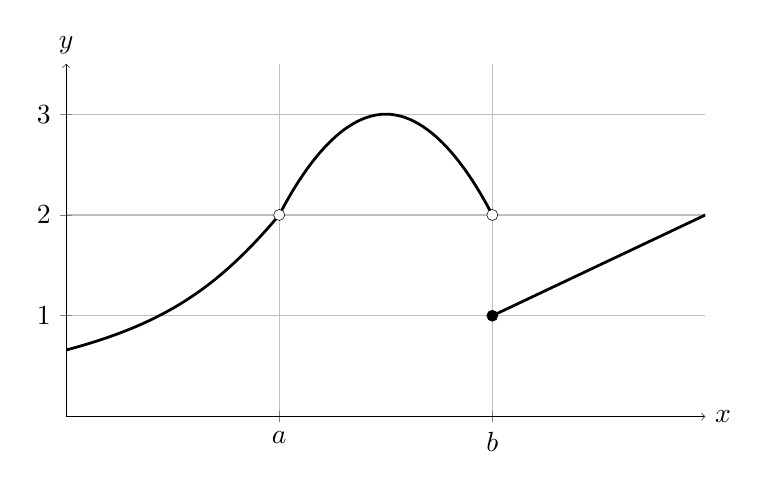
\begin{tikzpicture}
        \begin{axis}[
            axis y line=middle,
            axis x line=middle,
            axis line style={->},
            xlabel={$x$},
            xtick={1,2},
            xticklabels={$a$,$b$},
            x label style={
                at={(current axis.right of origin)},
                anchor=west,
            },
            ylabel={$y$},
            y label style={
                at={(current axis.above origin)},
                anchor=south,
            },
            ytick={1,2,3},
            xmin=0,xmax=3,
            ymin=0,ymax=3.5,
            width=0.8\columnwidth,
            height=0.5\columnwidth,
            very thin,
            grid=major,
        ]
        \draw[line width=1pt] (axis cs:0,0.66) to[out=15,in=230] (axis cs:1,2);
        \draw[line width=1pt] (axis cs:1,2) parabola bend (axis cs:1.5,3) (axis cs:2,2);
        \draw[fill=white] (axis cs:1,2) circle (2pt);
        \draw[fill=white] (axis cs:2,2) circle (2pt);
        \draw[fill=black] (axis cs:2,1) circle (2pt);
        \draw[line width=1pt] (axis cs:2,1) to (axis cs:3,2);
        \node[anchor=north east] at (axis cs:0,0) {0};
        \end{axis}
    \end{tikzpicture}
    \end{center}
    Which of the following statements about $f$ is true?
    %\begin{multicols}{2}
    \begin{choices}
        \wrongchoice{$\displaystyle \lim_{x\to a} f(x) = \lim_{x\to b} f(x)$}
      \correctchoice{$\displaystyle \lim_{x\to a} f(x) = 2$}
        \wrongchoice{$\displaystyle \lim_{x\to b} f(x) = 2$}
        \wrongchoice{$\displaystyle \lim_{x\to b} f(x) = 1$}
        \wrongchoice{$\displaystyle \lim_{x\to a} f(x)$ does not exist}
    \end{choices}
    %\end{multicols}
\end{question}
}

\element{calculusAB}{
\begin{question}{1997-AB-q16}
    The area of the region enclosed  by the graph of $y=x^2+1$ and the line $y=5$ is:
    \begin{multicols}{3}
    \begin{choices}
        \wrongchoice{$\dfrac{14}{3}$}
        \wrongchoice{$\dfrac{16}{3}$}
        \wrongchoice{$\dfrac{28}{3}$}
      \correctchoice{$\dfrac{32}{3}$}
        \wrongchoice{$8\pi$}
    \end{choices}
    \end{multicols}
\end{question}
}

\element{calculusAB}{
\begin{question}{1997-AB-q17}
    If $x^2 + y^2 = 25$, what is the value of $\dfrac{\mathrm{d}^2y}{\mathrm{d}x^2}$ at the point $(4,3)$?
    \begin{multicols}{3}
    \begin{choices}
      \correctchoice{$-\dfrac{25}{27}$}
        \wrongchoice{$-\dfrac{7}{27}$}
        \wrongchoice{$\dfrac{7}{27}$}
        \wrongchoice{$\dfrac{3}{4}$}
        \wrongchoice{$\dfrac{25}{27}$}
    \end{choices}
    \end{multicols}
\end{question}
}

\element{calculusAB}{
\begin{question}{1997-AB-q18}
    %% NOTE: TODO: dfrac in integral
    $\displaystyle\int^{\;\;\frac{\pi}{4}}_{0}\,\dfrac{\mathrm{e}^{\tan x}}{\cos^2 x}\,\mathrm{d}x = $
    \begin{multicols}{3}
    \begin{choices}
        \wrongchoice{$-\dfrac{25}{27}$}
        \wrongchoice{$-\dfrac{7}{27}$}
      \correctchoice{$\dfrac{7}{27}$}
        \wrongchoice{$\dfrac{3}{4}$}
        \wrongchoice{$\dfrac{25}{27}$}
    \end{choices}
    \end{multicols}
\end{question}
}

\element{calculusAB}{
\begin{question}{1997-AB-q19}
    If $f(x) = \ln \left|x^2-1\right|$,
        then $f\prime{}(x) = $
    \begin{multicols}{2}
    \begin{choices}
        \wrongchoice{$\left|\dfrac{2x}{x^2-1}\right|$}
        \wrongchoice{$\dfrac{2x}{\left|x^2-1\right|}$}
        \wrongchoice{$\dfrac{2\left|x\right|}{x^2-1}$}
      \correctchoice{$\dfrac{2x}{x^2-1}$}
        \wrongchoice{$\dfrac{1}{x^2-1}$}
    \end{choices}
    \end{multicols}
\end{question}
}

\element{calculusAB}{
\begin{question}{1997-AB-q20}
    The average value of $\cos x$ on the interval $\left[-3,5\right]$ is
    \begin{multicols}{2}
    \begin{choices}
        \wrongchoice{$\dfrac{\sin 6 - \sin 3}{8}$}
        \wrongchoice{$\dfrac{\sin 6 - \sin 3}{2}$}
        \wrongchoice{$\dfrac{\sin 3 - \sin 5}{2}$}
        \wrongchoice{$\dfrac{\sin 3 - \sin 5}{2}$}
      \correctchoice{$\dfrac{\sin 3 - \sin 5}{8}$}
    \end{choices}
    \end{multicols}
\end{question}
}

\element{calculusAB}{
\begin{question}{1997-AB-q21}
    $\displaystyle \lim_{x\to 1}\,\frac{x}{\ln x} =$
    \begin{multicols}{2}
    \begin{choices}
        \wrongchoice{$0$}
        \wrongchoice{$\dfrac{1}{\mathrm{e}}$}
        \wrongchoice{$1$}
        \wrongchoice{$\mathrm{e}$}
      \correctchoice{nonexistent}
    \end{choices}
    \end{multicols}
\end{question}
}

\element{calculusAB}{
\begin{question}{1997-AB-q22}
    What are all the values of $x$ for which the function $f$ defined by $f(x) = (x^2-3) \mathrm{e}^{-x}$ is increasing?
    \begin{choices}
        \wrongchoice{There aer no such values of $x$}
        \wrongchoice{$x<-1$ and $x>3$}
        \wrongchoice{$-3 < x < 1$}
      \correctchoice{$-1 < x < 3$}
        \wrongchoice{All values of $x$}
    \end{choices}
\end{question}
}

\element{calculusAB}{
\begin{question}{1997-AB-q23}
    If the region enclosed by the $y$-axis,
        the line $y=2$,
        and the curve $y=\sqrt{x}$ is revolved about the $y$-axis,
        the volume of the solid generated is:
    \begin{multicols}{3}
    \begin{choices}
      \correctchoice{$\dfrac{32\pi}{5}$}
        \wrongchoice{$\dfrac{16\pi}{3}$}
        \wrongchoice{$\dfrac{16\pi}{5}$}
        \wrongchoice{$\dfrac{8\pi}{3}$}
        \wrongchoice{$\pi$}
    \end{choices}
    \end{multicols}
\end{question}
}

\element{calculusAB}{
\begin{question}{1997-AB-q24}
    The expression
    \begin{equation*}
        \frac{1}{50} \left( \sqrt{\frac{1}{50}}
            + \sqrt{\frac{2}{50}}
            + \sqrt{\frac{3}{50}}
            + \cdots + \sqrt{\frac{50}{50}} + \right)
    \end{equation*}
    is a Riemann sum approximation for:
    \begin{multicols}{2}
    \begin{choices}
        \wrongchoice{$\displaystyle \int^{\;\;1}_0\,\sqrt{\frac{x}{50}}\,\mathrm{d}x$}
      \correctchoice{$\displaystyle \int^{\;\;1}_0\,\sqrt{x}\,\mathrm{d}x$}
        \wrongchoice{$\displaystyle \frac{1}{50} \int^{\;\;1}_0\,\sqrt{\frac{x}{50}}\,\mathrm{d}x$}
        \wrongchoice{$\displaystyle \frac{1}{50} \int^{\;\;1}_0\,\sqrt{x}\,\mathrm{d}x$}
        \wrongchoice{$\displaystyle \frac{1}{50} \int^{\;\;50}_0\,\sqrt{x}\,\mathrm{d}x$}
    \end{choices}
    \end{multicols}
\end{question}
}

\element{calculusAB}{
\begin{question}{1997-AB-q25}
    $\displaystyle \int x \sin\left(2x\right)\,\mathrm{d}x =$
    \begin{choices}
      \correctchoice{$-\dfrac{x}{2}\cos\left(2x\right) + \dfrac{1}{4}\sin\left(2x\right) + C$}
        \wrongchoice{$-\dfrac{x}{2}\cos\left(2x\right) - \dfrac{1}{4}\sin\left(2x\right) + C$}
        \wrongchoice{$\dfrac{x}{2}\cos\left(2x\right) - \dfrac{1}{4}\sin\left(2x\right) + C$}
        \wrongchoice{$-2x\cos\left(2x\right) + \sin\left(2x\right) + C$}
        \wrongchoice{$-2x\cos\left(2x\right) - 4\sin\left(2x\right) + C$}
    \end{choices}
\end{question}
}

\element{calculusAB}{
\begin{question}{1997-AB-q76}
    If $f(x) = \dfrac{\mathrm{e}^{2x}}{2x}$, then $f\prime{}(x)=$
    \begin{multicols}{2}
    \begin{choices}
        \wrongchoice{1}
        \wrongchoice{$\dfrac{\mathrm{e}^{2x}\left(1-2x\right)}{2x^2}$}
        \wrongchoice{$\mathrm{e}^{2x}$}
        \wrongchoice{$\dfrac{\mathrm{e}^{2x}\left(2x+1\right)}{x^2}$}
      \correctchoice{$\dfrac{\mathrm{e}^{2x}\left(2x-1\right)}{2x^2}$}
    \end{choices}
    \end{multicols}
\end{question}
}

\element{calculusAB}{
\begin{question}{1997-AB-q77}
    The graph of the function $y=x^3 + 6x^2 + 7x - 2\cos x$ changes concavity at $x=$
    \begin{multicols}{3}
    \begin{choices}
        \wrongchoice{$-1.58$}
        \wrongchoice{$-1.63$}
        \wrongchoice{$-1.67$}
      \correctchoice{$-1.89$}
        \wrongchoice{$-2.33$}
    \end{choices}
    \end{multicols}
\end{question}
}

\element{calculusAB}{
\begin{question}{1997-AB-q78}
    The graph of $f$ is shown in the figure below.
    \begin{center}
    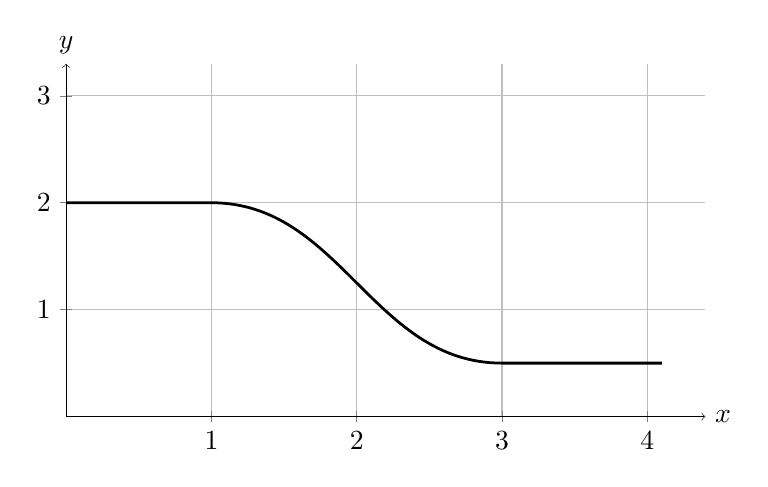
\begin{tikzpicture}
        \begin{axis}[
            axis y line=middle,
            axis x line=middle,
            axis line style={->},
            xlabel={$x$},
            xtick={0,1,2,3,4},
            x label style={
                at={(current axis.right of origin)},
                anchor=west,
            },
            ylabel={$y$},
            y label style={
                at={(current axis.above origin)},
                anchor=south,
            },
            ytick={0,1,2,3},
            xmin=0,xmax=4.4,
            ymin=0,ymax=3.3,
            width=0.8\columnwidth,
            height=0.5\columnwidth,
            grid=major,
            very thin,
        ]
        \draw[line width=1pt] (axis cs:0,2) to[out=0,in=180] (axis cs:1,2) to[out=0,in=180] (axis cs:3,0.5) to (axis cs:4.1,0.5);
        \end{axis}
    \end{tikzpicture}
    \end{center}
    If $\int^{\,3}_{1} f(x)\,\mathrm{d}x=2.3$ and $F\prime{}(x)=f(x)$,
        then $F(3) - F(0) =$
    \begin{multicols}{3}
    \begin{choices}
        \wrongchoice{$0.3$}
        \wrongchoice{$1.3$}
        \wrongchoice{$3.3$}
      \correctchoice{$4.3$}
        \wrongchoice{$5.3$}
    \end{choices}
    \end{multicols}
\end{question}
}

\element{calculusAB}{
\begin{questionmult}{1997-AB-q79}
    Let $f$ be a function such that
    \begin{equation*}
        \displaystyle \lim_{h\to 0} \frac{f(2+h) - f(2)}{h} = 5\,.
    \end{equation*}
    Which of the following must be true?
    \begin{choices}
      \correctchoice{$f$ is continuous at $x=2$}
      \correctchoice{$f$ is differentiable at $x=2$}
        \wrongchoice{The derivative of $f$ is continuous at $x=2$}
    \end{choices}
\end{questionmult}
}

\element{calculusAB}{
\begin{question}{1997-AB-q80}
    Let $f$ be a function given by $f(x) = 2\mathrm{e}^{4x^2}$.
    For what value of $x$ is the slope of the line tangent to the graph of $f$ at $\left(x,f(x)\right)$ equal to $3$?
    \begin{multicols}{3}
    \begin{choices}
      \correctchoice{$0.168$}
        \wrongchoice{$0.276$}
        \wrongchoice{$0.318$}
        \wrongchoice{$0.342$}
        \wrongchoice{$0.551$}
    \end{choices}
    \end{multicols}
\end{question}
}

\element{calculusAB}{
\begin{question}{1997-AB-q81}
    A railroad track and a road cross at right angles.
    An observer stands on the road 70 meters south of the crossing and watches an eastbound train traveling at 60 meters per second.
    At how many meters per second is the train moving away from the observer 4 seconds after is passes through the intersection?
    \begin{multicols}{3}
    \begin{choices}
      \correctchoice{$57.60$}
        \wrongchoice{$57.88$}
        \wrongchoice{$59.20$}
        \wrongchoice{$60.00$}
        \wrongchoice{$67.40$}
    \end{choices}
    \end{multicols}
\end{question}
}

\element{calculusAB}{
\begin{question}{1997-AB-q82}
    If $y=2x-8$, what is the minimum value of the product $xy$?
    \begin{multicols}{3}
    \begin{choices}
        \wrongchoice{$-16$}
      \correctchoice{$-8$}
        \wrongchoice{$-4$}
        \wrongchoice{$0$}
        \wrongchoice{$2$}
    \end{choices}
    \end{multicols}
\end{question}
}

\element{calculusAB}{
\begin{question}{1997-AB-q83}
    What is the area of the region in the first quadrant enclosed by the graphs of $y=\cos x$, $y=x$, and the $y$-axis?
    \begin{multicols}{3}
    \begin{choices}
        \wrongchoice{$0.127$}
        \wrongchoice{$0.385$}
      \correctchoice{$0.400$}
        \wrongchoice{$0.600$}
        \wrongchoice{$0.947$}
    \end{choices}
    \end{multicols}
\end{question}
}

\element{calculusAB}{
\begin{question}{1997-AB-q84}
    The base of a solid $S$ is the region enclosed by the graph of $y=\sqrt{\ln x}$,
        the line $x=\mathrm{e}$, and the $x$-axis.
    If the cross sections of $S$ perpendicular to the $x$-axis are squares,
        then the volume $S$ is:
    \begin{multicols}{3}
    \begin{choices}
        \wrongchoice{$\dfrac{1}{2}$}
        \wrongchoice{$\dfrac{2}{3}$}
      \correctchoice{$1$}
        \wrongchoice{$2$}
        \wrongchoice{$\dfrac{1}{3}\left(\mathrm{e}^2-1\right)$}
    \end{choices}
    \end{multicols}
\end{question}
}

\element{calculusAB}{
\begin{question}{1997-AB-q85}
    If the derivative of $f$ is given by $f\prime{}(x)=\mathrm{e}^2-3x^2$,
        at which of the following values of $x$ does $f$ have a relative maximum value?
    \begin{multicols}{3}
    \begin{choices}
        \wrongchoice{$-0.46$}
        \wrongchoice{$0.20$}
      \correctchoice{$0.91$}
        \wrongchoice{$0.95$}
        \wrongchoice{$3.73$}
    \end{choices}
    \end{multicols}
\end{question}
}

\element{calculusAB}{
\begin{question}{1997-AB-q86}
    Let $f(x) = \sqrt{x}$.
    If the rate of change of $f$ at $x=c$ is twice the rate of change at $x=1$, then $c=$
    \begin{multicols}{3}
    \begin{choices}
      \correctchoice{$\dfrac{1}{4}$}
        \wrongchoice{$1$}
        \wrongchoice{$4$}
        \wrongchoice{$\dfrac{1}{\sqrt{2}}$}
        \wrongchoice{$\dfrac{1}{2\sqrt{2}}$}
    \end{choices}
    \end{multicols}
\end{question}
}

\element{calculusAB}{
\begin{question}{1997-AB-q87}
    At time $t\geq 0$,
        the acceleration of a particle moving on the $x$-axis is $a(t) = t + \sin t$.
    At $t=0$, the velocity of the particle is $-2$.
    For what value $t$ will the velocity of the particle be zero?
    \begin{multicols}{3}
    \begin{choices}
        \wrongchoice{$1.02$}
      \correctchoice{$1.48$}
        \wrongchoice{$1.85$}
        \wrongchoice{$2.81$}
        \wrongchoice{$3.14$}
    \end{choices}
    \end{multicols}
\end{question}
}

\element{calculusAB}{
\begin{question}{1997-AB-q88}
    Let $f(x) = \int^{\,x}_{a} h(t)\,\mathrm{d}t$, where $h$ has the graph shown below.
    \begin{center}
    \begin{tikzpicture}
        \begin{axis}[
            axis y line=middle,
            axis x line=middle,
            axis line style={->},
            xlabel={$x$},
            xtick={-1.66,0,2,4},
            xticklabels={$a$,0,$b$,$c$},
            x label style={
                at={(current axis.right of origin)},
                anchor=west,
            },
            ylabel={$y$},
            y label style={
                at={(current axis.above origin)},
                anchor=south,
            },
            ytick=\empty,
            xmin=-2,xmax=4.4,
            ymin=-3,ymax=5,
            width=0.8\columnwidth,
            height=0.5\columnwidth,
            very thin,
        ]
        \addplot[line width=1pt,domain=-1.66:4] { 0.2 * (x+2) * (x-2) * (x-4)  };
        \end{axis}
    \end{tikzpicture}
    \end{center}
    Which of the following could be the graph of $f$?
    \begin{multicols}{2}
    \begin{choices}
        %% NOTE: changed options
        \AMCboxDimensions{down=-2.5em}
        \wrongchoice{
            \begin{tikzpicture}
                \begin{axis}[
                    axis y line=middle,
                    axis x line=middle,
                    axis line style={->},
                    xlabel={$x$},
                    xtick={-1.66,0,2,4},
                    xticklabels={$a$,0,$b$,$c$},
                    x label style={
                        at={(current axis.right of origin)},
                        anchor=west,
                    },
                    ylabel={$y$},
                    y label style={
                        at={(current axis.above origin)},
                        anchor=south,
                    },
                    ytick=\empty,
                    xmin=-2,xmax=4.4,
                    ymin=-3,ymax=5,
                    width=1.0\columnwidth,
                    very thin,
                ]
                %% made 1.66 a root
                \addplot[line width=1pt,domain=-1.66:4] { 0.2 * (x+1.66) * (x-2) * (x-4)  };
                \end{axis}
            \end{tikzpicture}
        }
        \wrongchoice{
            \begin{tikzpicture}
                \begin{axis}[
                    axis y line=middle,
                    axis x line=middle,
                    axis line style={->},
                    xlabel={$x$},
                    xtick={-1.66,0,2,4},
                    xticklabels={$a$,0,$b$,$c$},
                    x label style={
                        at={(current axis.right of origin)},
                        anchor=west,
                    },
                    ylabel={$y$},
                    y label style={
                        at={(current axis.above origin)},
                        anchor=south,
                    },
                    ytick=\empty,
                    xmin=-2,xmax=4.4,
                    ymin=-5,ymax=5,
                    width=1.0\columnwidth,
                    very thin,
                ]
                %% NOTE: absolute of h
                \addplot[line width=1pt,domain=-1.66:4] { abs(0.2 * (x+2) * (x-2) * (x-4)) };
                \end{axis}
            \end{tikzpicture}
        }
        \wrongchoice{
            \begin{tikzpicture}
                \begin{axis}[
                    axis y line=middle,
                    axis x line=middle,
                    axis line style={->},
                    xlabel={$x$},
                    xtick={-1.66,0,2,4},
                    xticklabels={$a$,0,$b$,$c$},
                    x label style={
                        at={(current axis.right of origin)},
                        anchor=west,
                    },
                    ylabel={$y$},
                    y label style={
                        at={(current axis.above origin)},
                        anchor=south,
                    },
                    ytick=\empty,
                    xmin=-2,xmax=4.4,
                    ymin=-5,ymax=5,
                    width=1.0\columnwidth,
                    very thin,
                ]
                %% NOTE: negative of h
                \addplot[line width=1pt,domain=-1.66:4] { -0.2 * (x+2) * (x-2) * (x-4) };
                \end{axis}
            \end{tikzpicture}
        }
        \wrongchoice{
            \begin{tikzpicture}
                \begin{axis}[
                    axis y line=middle,
                    axis x line=middle,
                    axis line style={->},
                    xlabel={$x$},
                    xtick={-1.66,0,2,4},
                    xticklabels={$a$,0,$b$,$c$},
                    x label style={
                        at={(current axis.right of origin)},
                        anchor=west,
                    },
                    ylabel={$y$},
                    y label style={
                        at={(current axis.above origin)},
                        anchor=south,
                    },
                    ytick=\empty,
                    xmin=-2,xmax=4.4,
                    ymin=-3,ymax=5,
                    width=1.0\columnwidth,
                    very thin,
                ]
                %% NOTE: derivative of h
                \addplot[line width=1pt,domain=-1.66:4] { 0.2 * ( (3*x^2) - (8*x) - 4 ) };
                \end{axis}
            \end{tikzpicture}
        }
        %% ANS is E
        \correctchoice{
            \begin{tikzpicture}
                \begin{axis}[
                    axis y line=middle,
                    axis x line=middle,
                    axis line style={->},
                    xlabel={$x$},
                    xtick={-1.66,0,2,4},
                    xticklabels={$a$,0,$b$,$c$},
                    x label style={
                        at={(current axis.right of origin)},
                        anchor=west,
                    },
                    ylabel={$y$},
                    y label style={
                        at={(current axis.above origin)},
                        anchor=south,
                    },
                    ytick=\empty,
                    xmin=-2,xmax=4.4,
                    ymin=-3,ymax=5,
                    width=1.0\columnwidth,
                    very thin,
                ]
                %% NOTE: integral of h + C
                \addplot[line width=1pt,domain=-1.66:4] { 2.50 + 0.1 * ( (0.25*x^4) - (1.33*x^3) - (2*x^2) + (16*x) ) };
                \end{axis}
            \end{tikzpicture}
        }
    \end{choices}
    \end{multicols}
\end{question}
}

\element{calculusAB}{
\begin{question}{1997-AB-q89}
    A table of values for a continous function $f$ is shown below.
    \begin{center}
    \begin{tabular}{lccccc}
        $x$    & 0  & 0.5 & 1.0 & 1.5 & 2.0 \\
        $f(x)$ & 3  & 5   & 5   & 8   & 13 \\
    \end{tabular}
    \end{center}
    If four equal subintervals of $\left[0,2\right]$ are used,
        which of the following is the trapexoidal approximation of $\int^{\,\,2}_{0}f(x)\,\mathrm{d}x$?
    \begin{multicols}{3}
    \begin{choices}
        \wrongchoice{8}
      \correctchoice{12}
        \wrongchoice{16}
        \wrongchoice{24}
        \wrongchoice{32}
    \end{choices}
    \end{multicols}
\end{question}
}

\element{calculusAB}{
\begin{questionmult}{1997-AB-q90}
    Which of the following are antiderivatives of $f(x) = \sin x \cos x$?
    \begin{choices}
      \correctchoice{$F(x) = \dfrac{\sin^2 x}{2}$}
        \wrongchoice{$F(x) = \dfrac{\cos^2 x}{2}$}
      \correctchoice{$F(x) = \dfrac{-\cos\left(2 x\right)}{4}$}
    \end{choices}
\end{questionmult}
}



%% 1998 AP Calculus AB: Section I (pp. 131)
%%--------------------------------------------------
\element{calculusAB}{
\begin{question}{1998-AB-q01}
    What is the $x$-coordinate of the point of inflection on the graph of $y=\dfrac{1}{3} x^3 + 5x^2 + 24$?
    \begin{multicols}{3}
    \begin{choices}
        \wrongchoice{$5$}
        \wrongchoice{zero}
        \wrongchoice{$-\dfrac{10}{3}$}
      \correctchoice{$-5$}
        \wrongchoice{$-10$}
    \end{choices}
    \end{multicols}
\end{question}
}

\element{calculusAB}{
\begin{question}{1998-AB-q02}
    The graph of a piecewise-linear function $f$, for $-1\leq x \leq 4$, is shown below.
    \begin{center}
    \begin{tikzpicture}
        \begin{axis}[
            axis y line=middle,
            axis x line=middle,
            axis line style={->},
            xlabel={$x$},
            xtick={-1,0,1,2,3,4},
            x label style={
                at={(current axis.right of origin)},
                anchor=west,
            },
            ylabel={$y$},
            y label style={
                at={(current axis.above origin)},
                anchor=south,
            },
            ytick={-2,-1,0,1,2},
            xmin=-1.4,xmax=4.4,
            ymin=-2.4,ymax=2.4,
            width=1.0\columnwidth,
            height=0.619\columnwidth,
            very thin,
        ]
        \addplot[line width=1pt,mark=*] plot coordinates { (-1,0) (0,2) (1,2) (2,0) (3,-1) (4,-1)};
        \end{axis}
    \end{tikzpicture}
    \end{center}
    %% NOTE: TODO: double check spacing on int bounds
    What is the value of $\displaystyle\int^{\;\;4}_{-1} f(x)\,\mathrm{d}x$?
    \begin{multicols}{3}
    \begin{choices}
        \wrongchoice{1}
      \correctchoice{2.5}
        \wrongchoice{4}
        \wrongchoice{5.5}
        \wrongchoice{8}
    \end{choices}
    \end{multicols}
\end{question}
}

\element{calculusAB}{
\begin{question}{1998-AB-q03}
    $\displaystyle \int^{\;\;2}_1\,\frac{1}{x^2}\,\mathrm{d}x =$
    \begin{multicols}{3}
    \begin{choices}
        \wrongchoice{$\dfrac{-1}{2}$}
        \wrongchoice{$\dfrac{7}{24}$}
      \correctchoice{$\dfrac{1}{2}$}
        \wrongchoice{$1$}
        \wrongchoice{$2\ln 2$}
    \end{choices}
    \end{multicols}
\end{question}
}

\element{calculusAB}{
\begin{question}{1998-AB-q04}
    If $f$ is continuous for $a\leq x \leq b$ and differentiable for $a<x<b$,
        which of the following could be false?
    \begin{choices}
        \wrongchoice{$f\prime{}(c) = \dfrac{f(b)-f(a)}{b-a}$ for some $c$ such that $a<c<b$}
      \correctchoice{$f\prime{}(c) = 0$ for some $c$ such that $a<c<b$}
        \wrongchoice{$f$ has a minimum value on $a\leq x\leq b$}
        \wrongchoice{$f$ has a maximum value on $a\leq x\leq b$}
        \wrongchoice{$\int^{\,b}_a f(x)\,\mathrm{d}x$ exists}
    \end{choices}
\end{question}
}

\element{calculusAB}{
\begin{question}{1998-AB-q05}
    $\displaystyle \int^{\;\;x}_0\,\sin t\,\mathrm{d}t = $
    \begin{multicols}{3}
    \begin{choices}
        \wrongchoice{$\sin x$}
        \wrongchoice{$-\cos x$}
        \wrongchoice{$\cos x$}
        \wrongchoice{$\cos x - 1$}
      \correctchoice{$1- \cos x$}
    \end{choices}
    \end{multicols}
\end{question}
}

\element{calculusAB}{
\begin{question}{1998-AB-q06}
    If $x^2 + xy=10$,
        then when $x=2$, $\dfrac{\mathrm{d}y}{\mathrm{d}x} = $
    \begin{multicols}{3}
    \begin{choices}
      \correctchoice{$-\dfrac{7}{2}$}
        \wrongchoice{$-2$}
        \wrongchoice{$\dfrac{2}{7}$}
        \wrongchoice{$\dfrac{3}{2}$}
        \wrongchoice{$\dfrac{7}{2}$}
    \end{choices}
    \end{multicols}
\end{question}
}

\element{calculusAB}{
\begin{question}{1998-AB-q07}
    $\displaystyle \int^{\;\;\mathrm{e}}_1\,\left(\frac{x^2-1}{x}\right)\,\mathrm{d}x = $
    \begin{multicols}{3}
    \begin{choices}
        \wrongchoice{$\mathrm{e} - \dfrac{1}{\mathrm{e}}$}
        \wrongchoice{$\mathrm{e}^2 - \mathrm{e}$}
        \wrongchoice{$\dfrac{\mathrm{e}^2}{2} - \mathrm{e} + \dfrac{1}{2}$}
        \wrongchoice{$\mathrm{e}^2 -2$}
      \correctchoice{$\dfrac{\mathrm{e}^2}{2} - \dfrac{3}{2}$}
    \end{choices}
    \end{multicols}
\end{question}
}

\element{calculusAB}{
\begin{question}{1998-AB-q08}
    Let $f$ and $g$ be differentiable functions with the following properties:
    \begin{center}
    \begin{tabular}{ccl}
        (i)  & &  $g(x)>0$ for all $x$ \\
        (ii) & &  $f(0) = 1$ \\
    \end{tabular}
    \end{center}
    If $h(x)=f(x)g(x)$ and $h\prime{}(x) = f(x) g\prime{}(x)$,
        then $f(x) = $
    \begin{multicols}{3}
    \begin{choices}
        \wrongchoice{$f\prime{}(x)$}
        \wrongchoice{$g(x)$}
        \wrongchoice{$\mathrm{e}^{x}$}
        \wrongchoice{zero}
      \correctchoice{one}
    \end{choices}
    \end{multicols}
\end{question}
}

\element{calculusAB}{
\begin{question}{1998-AB-q09}
    The flow of oil, in barrels per hour, through a pipeline on July 9 is given by the graph shown below.
    \begin{center}
    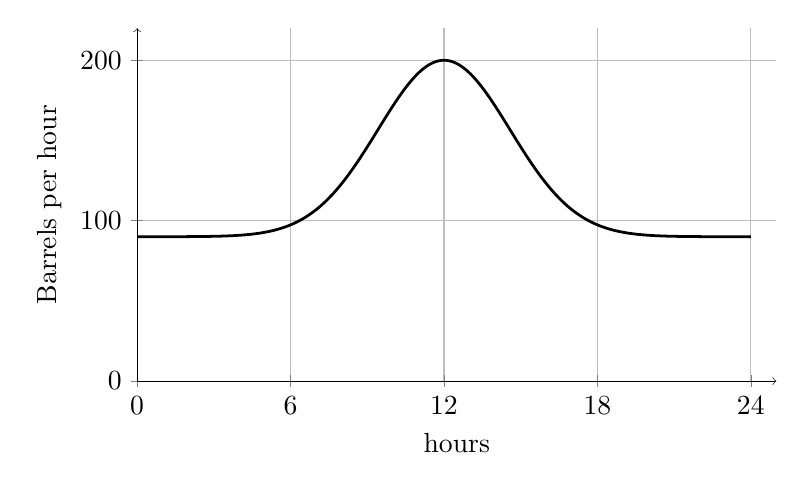
\begin{tikzpicture}
        \begin{axis}[
            axis y line=left,
            axis x line=bottom,
            axis line style={->},
            xlabel={hours},
            xtick={0,6,12,18,24},
            ylabel={Barrels per hour},
            ytick={0,100,200},
            xmin=0,xmax=25,
            ymin=0,ymax=220,
            width=0.8\columnwidth,
            height=0.5\columnwidth,
            very thin,
            grid=major,
        ]
        \addplot[line width=1pt,domain=0:24,samples=200] {90 + 110 * exp( -0.075*(x-12)^2 ) };
        \end{axis}
    \end{tikzpicture}
    \end{center}
    Of the following, which best approximates the total number of barrels of oil that passes through the pipeline that day?
    \begin{multicols}{3}
    \begin{choices}
        \wrongchoice{500}
        \wrongchoice{600}
        \wrongchoice{\num{2 400}}
      \correctchoice{\num{3 000}}
        \wrongchoice{\num{4 800}}
    \end{choices}
    \end{multicols}
\end{question}
}

\element{calculusAB}{
\begin{question}{1998-AB-q10}
    What is the instantaneous rate of change at $x=2$ of the function $f$ given by $f(x) = \dfrac{x^2-2}{x-1}$?
    \begin{multicols}{3}
    \begin{choices}
        \wrongchoice{$-2$}
        \wrongchoice{$\dfrac{1}{6}$}
        \wrongchoice{$\dfrac{1}{2}$}
      \correctchoice{$2$}
        \wrongchoice{$6$}
    \end{choices}
    \end{multicols}
\end{question}
}

\element{calculusAB}{
\begin{question}{1998-AB-q11}
    If $f$ is a linear function and $0<a<b$,
        then $\int^{\,b}_a\,f\dprime{}(x)\,\mathrm{d}x = $
    \begin{multicols}{3}
    \begin{choices}
      \correctchoice{$0$}
        \wrongchoice{$1$}
        \wrongchoice{$\dfrac{ab}{2}$}
        \wrongchoice{$b-a$}
        \wrongchoice{$\dfrac{b^2-a^2}{2}$}
    \end{choices}
    \end{multicols}
\end{question}
}

\element{calculusAB}{
\begin{question}{1998-AB-q12}
    If \begin{math}
        f(x) = 
        \begin{cases}
            \ln x       & \text{ for } 0<x\leq 2 \\
            x^2 \ln 2   & \text{ for } 2<x\leq 4 \\
        \end{cases}
    \end{math},
    then $\lim_{x\to 2} f(x)$ is:
    \begin{multicols}{2}
    \begin{choices}
        \wrongchoice{$\ln 2$}
        \wrongchoice{$\ln 8$}
        \wrongchoice{$\ln 16$}
        \wrongchoice{$4$}
      \correctchoice{nonexistent}
    \end{choices}
    \end{multicols}
\end{question}
}

\element{calculusAB}{
\begin{question}{1998-AB-q13}
    The graph of the function $f$ shown in the figure below has a vertical tangent at the point $(2,0)$ and horizontal tangents at the points $(1,-1)$ and $(3,1)$.
    \begin{center}
    \begin{tikzpicture}
        \begin{axis}[
            axis y line=middle,
            axis x line=middle,
            axis line style={->},
            xlabel={$x$},
            xtick={-2,-1,0,1,2,3,4},
            x label style={
                at={(current axis.right of origin)},
                anchor=west,
            },
            ylabel={$y$},
            y label style={
                at={(current axis.above origin)},
                anchor=south,
            },
            ytick={-2,-1,0,1,2},
            xmin=-2.2,xmax=4.2,
            ymin=-2.2,ymax=2.2,
            width=0.8\columnwidth,
            %height=0.5\columnwidth,
            very thin,
        ]
        \draw[line width=1pt] (axis cs:0,0) arc (180:360:1) arc (180:0:1);
        \draw[line width=1pt] (axis cs:-2,1) to[out=290,in=160] (axis cs:0,-1);
        \draw[fill=white] (axis cs:0,-1) circle (2pt);
        \draw[fill=black] (axis cs:0,0) circle (2pt);
        \end{axis}
    \end{tikzpicture}
    \end{center}
    For what values of $x$, $-2<x<4$, is $f$ not differentiable?
    \begin{multicols}{2}
    \begin{choices}
        \wrongchoice{0 only}
      \correctchoice{0 and 2 only}
        \wrongchoice{1 and 3 only}
        \wrongchoice{0, 1, and 3 only}
        \wrongchoice{0, 1, 2 and 3}
    \end{choices}
    \end{multicols}
\end{question}
}

\element{calculusAB}{
\begin{question}{1998-AB-q14}
    A particle moves along the $x$-axis so that its position at time $t$ is given by $x(t)=t^2-6t+5$.
    For what value of $t$ is the velocity of the particle zero?
    \begin{multicols}{3}
    \begin{choices}
        \wrongchoice{1}
        \wrongchoice{2}
      \correctchoice{3}
        \wrongchoice{4}
        \wrongchoice{5}
    \end{choices}
    \end{multicols}
\end{question}
}

\element{calculusAB}{
\begin{question}{1998-AB-q15}
    If $F(x) = \int^{\,x}_0\sqrt{t^3+1}\,\mathrm{d}t$,
        then $F (2)=$
    \begin{multicols}{3}
    \begin{choices}
        \wrongchoice{$-3$}
        \wrongchoice{$-2$}
        \wrongchoice{$2$}
      \correctchoice{$3$}
        \wrongchoice{$18$}
    \end{choices}
    \end{multicols}
\end{question}
}

\element{calculusAB}{
\begin{question}{1998-AB-q16}
    If $f(x) = \sin\left(\mathrm{e}^{-x}\right)$,
        then $f\prime{}(x) = $
    \begin{multicols}{2}
    \begin{choices}
        \wrongchoice{$-\cos\left(\mathrm{e}^{-x}\right)$}
        \wrongchoice{$\cos\left(\mathrm{e}^{-x}\right) + \mathrm{e}^{-x}$}
        \wrongchoice{$\cos\left(\mathrm{e}^{-x}\right) - \mathrm{e}^{-x}$}
        \wrongchoice{$\mathrm{e}^{-x} \cos\left(\mathrm{e}^{-x}\right)$}
      \correctchoice{$-\mathrm{e}^{-x} \cos\left(\mathrm{e}^{-x}\right)$}
    \end{choices}
    \end{multicols}
\end{question}
}

\element{calculusAB}{
\begin{question}{1998-AB-q17}
    The graph of a twice-differentiable function $f$ is shown in the figure below.
    \begin{center}
    \begin{tikzpicture}
        \begin{axis}[
            axis y line=middle,
            axis x line=middle,
            axis line style={->},
            xlabel={$x$},
            xtick={0,1},
            x label style={
                at={(current axis.right of origin)},
                anchor=west,
            },
            ylabel={$y$},
            y label style={
                at={(current axis.above origin)},
                anchor=south,
            },
            ytick=\empty,
            xmin=-1,xmax=5,
            ymin=-2,ymax=2,
            width=0.8\columnwidth,
            height=0.5\columnwidth,
            very thin,
        ]
        \addplot[line width=1pt,samples=100] { -0.1*(x-1)*(x-10) };
        \end{axis}
    \end{tikzpicture}
    \end{center}
    Which of the following is true?
    \begin{choices}
        \wrongchoice{$f(1) < f\prime{}(1) < f\dprime{}(1)$}
        \wrongchoice{$f(1) < f\dprime{}(1) < f\prime{}(1)$}
        \wrongchoice{$f\prime{}(1) < f(1) < f\dprime{}(1)$}
      \correctchoice{$f\dprime{}(1) < f(1) < f\prime{}(1)$}
        \wrongchoice{$f\dprime{}(1) < f\prime (1) < f(1)$}
    \end{choices}
\end{question}
}

\element{calculusAB}{
\begin{question}{1998-AB-q18}
    An equation of the line tangent to the graph of $y= x + \cos x$ at the point $(0,1)$ is
    \begin{multicols}{2}
    \begin{choices}
        \wrongchoice{$y = 2x + 1$}
      \correctchoice{$y = x + 1$}
        \wrongchoice{$y = x$}
        \wrongchoice{$y = x - 1$}
        \wrongchoice{$y = 0$}
    \end{choices}
    \end{multicols}
\end{question}
}

\element{calculusAB}{
\begin{question}{1998-AB-q19}
    If $f\dprime (x) = x(x+1)(x-2)^2$, then the graph of $f$ has inflection points when $x=$
    \begin{multicols}{2}
    \begin{choices}
        \wrongchoice{$-1$ only}
        \wrongchoice{$2$ only}
      \correctchoice{$-1$ and $0$ only}
        \wrongchoice{$-1$ and $2$ only}
        \wrongchoice{$-1$, $0$, and $2$ only}
    \end{choices}
    \end{multicols}
\end{question}
}

\element{calculusAB}{
\begin{question}{1998-AB-q20}
    What are the values of $k$ for which $\displaystyle \int^{\;\;k}_{-3}\,x^2\,\mathrm{d} x = 0$?
    \begin{multicols}{2}
    \begin{choices}
      \correctchoice{$-3$}
        \wrongchoice{$0$}
        \wrongchoice{$3$}
        \wrongchoice{$-3$ and $3$}
        \wrongchoice{$-3$, $0$ and $3$}
    \end{choices}
    \end{multicols}
\end{question}
}

\element{calculusAB}{
\begin{question}{1998-AB-q21}
    If $\dfrac{\mathrm{d}y}{\mathrm{d}t} = ky$ and $k$ is a nonzero constant,
        then $y$ could be:
    \begin{multicols}{2}
    \begin{choices}
        \wrongchoice{$2 \mathrm{e}^{kty}$}
      \correctchoice{$2 \mathrm{e}^{kt}$}
        \wrongchoice{$\mathrm{e}^{kt} + 3$}
        \wrongchoice{$kty + 5$}
        \wrongchoice{$\dfrac{1}{2}ky^2 + \dfrac{1}{2}$}
    \end{choices}
    \end{multicols}
\end{question}
}

\element{calculusAB}{
\begin{question}{1998-AB-q22}
    The function $f$ is given by $f(x) = x^4 + x^2 - 2$.
    On which of the following intervals is $f$ increasing?
    \begin{multicols}{2}
    \begin{choices}
        \wrongchoice{$\left(-\dfrac{1}{\sqrt{2}},\infty\right)$}
        \wrongchoice{$\left(-\dfrac{1}{\sqrt{2}},\dfrac{1}{\sqrt{2}}\right)$}
      \correctchoice{$\left(0,\infty\right)$}
        \wrongchoice{$\left(-\infty,0\right)$}
        \wrongchoice{$\left(-\infty,-\dfrac{1}{\sqrt{2}}\right)$}
    \end{choices}
    \end{multicols}
\end{question}
}

\element{calculusAB}{
\begin{question}{1998-AB-q23}
    The graph of $f$ is shown in the figure below.
    \begin{center}
    \begin{tikzpicture}
        \begin{axis}[
            axis y line=middle,
            axis x line=middle,
            axis line style={->},
            xlabel={$x$},
            xtick={-3.74,0,5.74},
            xticklabels={$a$,0,$b$},
            x label style={
                at={(current axis.right of origin)},
                anchor=west,
            },
            ylabel={$y$},
            y label style={
                at={(current axis.above origin)},
                anchor=south,
            },
            ytick=\empty,
            xmin=-4,xmax=6,
            ymin=-3,ymax=3,
            width=0.8\columnwidth,
            height=0.5\columnwidth,
            very thin,
        ]
        \addplot[line width=1pt,samples=100,domain=-3.74:5.74] { 0.008 * (x+5) * (x+2) * (x-4) * (x-7) };
        \end{axis}
    \end{tikzpicture}
    \end{center}
    Which of the following could be the graph of the derivative of $f$
    \begin{multicols}{2}
    \begin{choices}
        \AMCboxDimensions{down=-2.0em}
        %% ANS is A
        \correctchoice{
            \begin{tikzpicture}
                \begin{axis}[
                    axis y line=middle,
                    axis x line=middle,
                    axis line style={->},
                    xlabel={$x$},
                    xtick={-3.74,0,5.74},
                    xticklabels={$a$,0,$b$},
                    x label style={
                        at={(current axis.right of origin)},
                        anchor=west,
                    },
                    ylabel={$y$},
                    y label style={
                        at={(current axis.above origin)},
                        anchor=south,
                    },
                    ytick=\empty,
                    xmin=-4,xmax=6,
                    ymin=-3,ymax=3,
                    width=1.0\columnwidth,
                    very thin,
                ]
                \addplot[line width=1pt,samples=100,domain=-3.74:5.74] { 0.05 * (x+3.74) * (x-1) * (x-5.74) };
                \end{axis}
            \end{tikzpicture}
        }
        \wrongchoice{
            \begin{tikzpicture}
                \begin{axis}[
                    axis y line=middle,
                    axis x line=middle,
                    axis line style={->},
                    xlabel={$x$},
                    xtick={-3.74,0,5.74},
                    xticklabels={$a$,0,$b$},
                    x label style={
                        at={(current axis.right of origin)},
                        anchor=west,
                    },
                    ylabel={$y$},
                    y label style={
                        at={(current axis.above origin)},
                        anchor=south,
                    },
                    ytick=\empty,
                    xmin=-4,xmax=6,
                    ymin=-3,ymax=3,
                    width=1.0\columnwidth,
                    very thin,
                ]
                \addplot[line width=1pt,samples=100,domain=-3.74:5.74] { abs(0.008 * (x+5) * (x+2) * (x-4) * (x-7)) };
                \end{axis}
            \end{tikzpicture}
        }
        \wrongchoice{
            \begin{tikzpicture}
                \begin{axis}[
                    axis y line=middle,
                    axis x line=middle,
                    axis line style={->},
                    xlabel={$x$},
                    xtick={-3.74,0,5.74},
                    xticklabels={$a$,0,$b$},
                    x label style={
                        at={(current axis.right of origin)},
                        anchor=west,
                    },
                    ylabel={$y$},
                    y label style={
                        at={(current axis.above origin)},
                        anchor=south,
                    },
                    ytick=\empty,
                    xmin=-4,xmax=6,
                    ymin=-3,ymax=3,
                    width=1.0\columnwidth,
                    very thin,
                ]
                \addplot[line width=1pt,samples=100,domain=-3.74:5.74] { -0.05 * (x+3.74) * (x-1) * (x-5.74) };
                \end{axis}
            \end{tikzpicture}
        }
        \wrongchoice{
            \begin{tikzpicture}
                \begin{axis}[
                    axis y line=middle,
                    axis x line=middle,
                    axis line style={->},
                    xlabel={$x$},
                    xtick={-3.74,0,5.74},
                    xticklabels={$a$,0,$b$},
                    x label style={
                        at={(current axis.right of origin)},
                        anchor=west,
                    },
                    ylabel={$y$},
                    y label style={
                        at={(current axis.above origin)},
                        anchor=south,
                    },
                    ytick=\empty,
                    xmin=-4,xmax=6,
                    ymin=-3,ymax=3,
                    width=1.0\columnwidth,
                    very thin,
                ]
                \addplot[line width=1pt,samples=100,domain=-3.74:5.74] { -0.008 * (x+5) * (x+2) * (x-4) * (x-7) };
                \end{axis}
            \end{tikzpicture}
        }
        \wrongchoice{
            \begin{tikzpicture}
                \begin{axis}[
                    axis y line=middle,
                    axis x line=middle,
                    axis line style={->},
                    xlabel={$x$},
                    xtick={-3.74,0,5.74},
                    xticklabels={$a$,0,$b$},
                    x label style={
                        at={(current axis.right of origin)},
                        anchor=west,
                    },
                    ylabel={$y$},
                    y label style={
                        at={(current axis.above origin)},
                        anchor=south,
                    },
                    ytick=\empty,
                    xmin=-4,xmax=6,
                    ymin=-3,ymax=3,
                    width=1.0\columnwidth,
                    very thin,
                ]
                \addplot[line width=1pt,samples=100,domain=-3.74:5.74] { -0.75*(x-1) };
                \end{axis}
            \end{tikzpicture}
        }
    \end{choices}
    \end{multicols}
\end{question}
}

\element{calculusAB}{
\begin{question}{1998-AB-q24}
    The maximum acceleration attained on the inerval $0 \leq t \leq 3$ by the particle whose velocity is given by $v(t) = t^3 - 3t^2 + 12t + 4$ is
    \begin{multicols}{3}
    \begin{choices}
        \wrongchoice{$9$}
        \wrongchoice{$12$}
        \wrongchoice{$14$}
      \correctchoice{$21$}
        \wrongchoice{$40$}
    \end{choices}
    \end{multicols}
\end{question}
}

\element{calculusAB}{
\begin{question}{1998-AB-q25}
    What is the area of the region between the graphs of $y=x^2$ and $y=-x$ from $x=0$ to $x=2$?
    \begin{multicols}{3}
    \begin{choices}
        \wrongchoice{$\dfrac{2}{3}$}
        \wrongchoice{$\dfrac{8}{3}$}
        \wrongchoice{$4$}
      \correctchoice{$\dfrac{14}{3}$}
        \wrongchoice{$\dfrac{16}{3}$}
    \end{choices}
    \end{multicols}
\end{question}
}

\element{calculusAB}{
\begin{question}{1998-AB-q26}
    The function $f$ is continous on the closed interval $\left[0,2\right]$ and has values that are given in the table below.
    \begin{center}
    \begin{tabular}{cccc}
        x    & 0 & 1   & 2 \\
        f(x) & 1 & $k$ & 2 \\
    \end{tabular}
    \end{center}
    The equation $f(x) = \dfrac{1}{2}$ must have at least two solutions in the interval $\left[0,2\right]$ if $k=$
    \begin{multicols}{3}
    \begin{choices}
      \correctchoice{$0$}
        \wrongchoice{$\dfrac{1}{2}$}
        \wrongchoice{$1$}
        \wrongchoice{$2$}
        \wrongchoice{$3$}
    \end{choices}
    \end{multicols}
\end{question}
}

\element{calculusAB}{
\begin{question}{1998-AB-q27}
    What is the average value of $y=x^2\sqrt{x^3+1}$ on the interval $\left[0,2\right]$?
    \begin{multicols}{3}
    \begin{choices}
      \correctchoice{$\dfrac{26}{9}$}
        \wrongchoice{$\dfrac{52}{9}$}
        \wrongchoice{$\dfrac{26}{3}$}
        \wrongchoice{$\dfrac{52}{3}$}
        \wrongchoice{$24$}
    \end{choices}
    \end{multicols}
\end{question}
}

\element{calculusAB}{
\begin{question}{1998-AB-q28}
    If $f(x)=\tan\left(2x\right)$, then $f\prime\left(\dfrac{\pi}{6}\right)=$
    \begin{multicols}{3}
    \begin{choices}
        \wrongchoice{$\sqrt{3}$}
        \wrongchoice{$2\sqrt{3}$}
        \wrongchoice{$4$}
        \wrongchoice{$4\sqrt{3}$}
      \correctchoice{$8$}
    \end{choices}
    \end{multicols}
\end{question}
}

\element{calculusAB}{
\begin{question}{1998-AB-q76}
    The graph of a function $f$ is shown below.
    \begin{center}
    \begin{tikzpicture}
        \begin{axis}[
            axis y line=middle,
            axis x line=middle,
            axis line style={->},
            xlabel={$x$},
            xtick={2},
            xticklabels={$a$},
            x label style={
                at={(current axis.right of origin)},
                anchor=west,
            },
            ylabel={$y$},
            y label style={
                at={(current axis.above origin)},
                anchor=south,
            },
            ytick=\empty,
            xmin=-3,xmax=6,
            ymin=-3,ymax=6,
            width=0.8\columnwidth,
            height=0.5\columnwidth,
            very thin,
        ]
        \addplot[line width=1pt,smooth,tension=0.5] plot coordinates { (-3,-2) (-1,0) (0,2) (2,3) (4,3) (5,5) };
        \draw[fill=white] (axis cs:2,3) circle (1.5pt);
        \draw[fill=black] (axis cs:2,5) circle (1.5pt);
        \end{axis}
    \end{tikzpicture}
    \end{center}
    Which of the following statements about $f$ is false?
    \begin{choices}
      \correctchoice{$f$ is continuous at $x=a$.}
        \wrongchoice{$f$ has a relative maximum at $x=a$.}
        \wrongchoice{$x=a$ is in the domain of $f$.}
        \wrongchoice{$\lim_{x\to a^+} f(x)$ is equal to $\lim_{x\to a^-} f(x)$.}
        \wrongchoice{$\lim_{x\to a} f(x)$ exists.}
    \end{choices}
\end{question}
}

\element{calculusAB}{
\begin{question}{1998-AB-q77}
    Let $f$ be the function given by $f(x) = 3\mathrm{e}^{2x}$ and let $g$ be the function given by $g(x)=6x^3$.
    At what value of $x$ do the graphs of $f$ and $g$ have parallel tangent lines?
    \begin{multicols}{3}
    \begin{choices}
        \wrongchoice{$-0.701$}
        \wrongchoice{$-0.567$}
      \correctchoice{$-0.391$}
        \wrongchoice{$-0.302$}
        \wrongchoice{$-0.258$}
    \end{choices}
    \end{multicols}
\end{question}
}

\element{calculusAB}{
\begin{question}{1998-AB-q78}
    The radius of a circle is decreasing at a constant rate of 0.1 centimeter per second.
    In terms of the circumference $C$,
        what is the rate of change of the area of the circle,
        in square centimeters per second?
    \begin{multicols}{3}
    \begin{choices}
        \wrongchoice{$-\left(0.2\right) \pi C$}
      \correctchoice{$-\left(0.1\right) \pi C$}
        \wrongchoice{$-\dfrac{\left(0.2\right)C}{2\pi}$}
        \wrongchoice{$\left(0.2\right)^2 C$}
        \wrongchoice{$\left(0.2\right)^2 \pi C$}
    \end{choices}
    \end{multicols}
\end{question}
}

\element{calculusAB}{
\begin{question}{1998-AB-q79}
    %The graphs of the derivatives of the functions $f$, $g$, and $h$ are shown below.
    %Which of the functions $f$, $g$, or $h$ have a relative maximum on the open interval $a<x<b$?
    %% NOTE: reworded
    The graphs of the derivatives of three functions are shown.
    Which of the functions have a relative maximum on the open interval $a<x<b$?
    %% NOTE: Questionmult make too difficult?
    \begin{choices}
        \AMCboxDimensions{down=-0.15\columnwidth}
        \correctchoice{
            \begin{tikzpicture}
                \begin{axis}[
                    axis y line=middle,
                    axis x line=middle,
                    axis line style={->},
                    xlabel={$x$},
                    xtick={-4,0,4},
                    xticklabels={$a$,0,$b$},
                    x label style={
                        at={(current axis.right of origin)},
                        anchor=west,
                    },
                    ylabel={$y$},
                    y label style={
                        at={(current axis.above origin)},
                        anchor=south,
                    },
                    ytick=\empty,
                    xmin=-5,xmax=5,
                    ymin=-5,ymax=5,
                    width=0.8\columnwidth,
                    height=0.5\columnwidth,
                    very thin,
                ]
                \addplot[line width=1pt,samples=100,domain=-5:5] { -0.1* (x+3)^2 * (x-1) * (x-3.5) };
                %\node[pin={40:$y=f\prime{}(x)$}] at (0,0) {};
                \end{axis}
            \end{tikzpicture}
        }
        \wrongchoice{
            \begin{tikzpicture}
                \begin{axis}[
                    axis y line=middle,
                    axis x line=middle,
                    axis line style={->},
                    xlabel={$x$},
                    xtick={-4,0,4},
                    xticklabels={$a$,0,$b$},
                    x label style={
                        at={(current axis.right of origin)},
                        anchor=west,
                    },
                    ylabel={$y$},
                    y label style={
                        at={(current axis.above origin)},
                        anchor=south,
                    },
                    ytick=\empty,
                    xmin=-5,xmax=5,
                    ymin=-5,ymax=5,
                    width=0.8\columnwidth,
                    height=0.5\columnwidth,
                    very thin,
                ]
                \addplot[line width=1pt,samples=100,domain=-5:5] { 4 * x * exp(-0.2*x^2) };
                %\node[pin={40:$y=g\prime{}(x)$}] at (0,0) {};
                \end{axis}
            \end{tikzpicture}
        }
        \wrongchoice{
            \begin{tikzpicture}
                \begin{axis}[
                    axis y line=middle,
                    axis x line=middle,
                    axis line style={->},
                    xlabel={$x$},
                    xtick={-4,0,4},
                    xticklabels={$a$,0,$b$},
                    x label style={
                        at={(current axis.right of origin)},
                        anchor=west,
                    },
                    ylabel={$y$},
                    y label style={
                        at={(current axis.above origin)},
                        anchor=south,
                    },
                    ytick=\empty,
                    xmin=-5,xmax=5,
                    ymin=-5,ymax=5,
                    width=0.8\columnwidth,
                    height=0.5\columnwidth,
                    very thin,
                ]
                \addplot[line width=1pt,samples=100,domain=-5:5] { 4 * exp(-0.2*x^2) };
                %\node[pin={40:$y=h\prime{}(x)$}] at (0,0) {};
                \end{axis}
            \end{tikzpicture}
        }
        %\correctchoice{$f$ only}
        %\wrongchoice{$g$ only}
        %\wrongchoice{$h$ only}
        %\wrongchoice{$f$ and $g$ only}
        %\wrongchoice{$f$, $g$ and $h$}
    \end{choices}
\end{question}
}

\element{calculusAB}{
\begin{question}{1998-AB-q80}
    The first derivative of the function $f$ is given by $f\prime{}(x)=\dfrac{\cos^2 x}{x} - \dfrac{1}{5}$.
    How many critical values does $f$ have on the open interval $\left(0,10\right)$?
    \begin{multicols}{3}
    \begin{choices}
        \wrongchoice{one}
      \correctchoice{three}
        \wrongchoice{four}
        \wrongchoice{five}
        \wrongchoice{seven}
    \end{choices}
    \end{multicols}
\end{question}
}

\element{calculusAB}{
\begin{questionmult}{1998-AB-q81}
    Let $f$ be the function given by $f(x) = \left|x\right|$.
    Which of the following statements about $f$ are true?
    \begin{choices}
      \correctchoice{$f$ is continuous at $x=0$}
        \wrongchoice{$f$ is differentiable at $x=0$}
      \correctchoice{$f$ has an absolute minimum at $x=0$}
    \end{choices}
\end{questionmult}
}

\element{calculusAB}{
\begin{question}{1998-AB-q82}
    If $f$ is a continuous function and if $F\prime{}(x)=f(x)$ for all real numbers $x$,
        then $\int^{\,3}_{1} f(2x)\,\mathrm{d}x = $
    \begin{multicols}{2}
    \begin{choices}
        \wrongchoice{$2 F(3) - 2 F(1)$}
        \wrongchoice{$\dfrac{1}{2} F(3) - \dfrac{1}{2} F(1)$}
        \wrongchoice{$2 F(6) - 2 F(2)$}
        \wrongchoice{$F(6) - F(2)$}
      \correctchoice{$\dfrac{1}{2} F(6) - \dfrac{1}{2} F(2)$}
    \end{choices}
    \end{multicols}
\end{question}
}

\element{calculusAB}{
\begin{question}{1998-AB-q83}
    If $a\neq 0$, then $\displaystyle \lim_{x\to a} \dfrac{x^2-a^2}{x^4-a^4}$ is:
    \begin{multicols}{2}
    \begin{choices}
        \wrongchoice{$\dfrac{1}{a^2}$}
      \correctchoice{$\dfrac{1}{2a^2}$}
        \wrongchoice{$\dfrac{1}{6a^2}$}
        \wrongchoice{zero}
        \wrongchoice{nonexistent}
    \end{choices}
    \end{multicols}
\end{question}
}

\element{calculusAB}{
\begin{question}{1998-AB-q84}
    Population $y$ grows according to the equation $\dfrac{\mathrm{d}y}{\mathrm{d}t} = ky$,
        where $k$ is a constant and $t$ is measured in years.
    If the population doubles every 10 years,
        then the value of $k$ is:
    \begin{multicols}{2}
    \begin{choices}
      \correctchoice{$0.069$}
        \wrongchoice{$0.200$}
        \wrongchoice{$0.301$}
        \wrongchoice{$3.322$}
        \wrongchoice{$5.000$}
    \end{choices}
    \end{multicols}
\end{question}
}

\element{calculusAB}{
\begin{question}{1998-AB-q85}
    The function $f$ is continous on the closed interval $\left[2,8\right]$ and has values that are given in the table below.
    \begin{center}
    \begin{tabular}{lcccc}
        $x$    & 2  & 5  & 7  & 8  \\
        $f(x)$ & 10 & 30 & 40 & 20 \\
    \end{tabular}
    \end{center}
    Using the subintervals $\left[2,5\right]$, $\left[5,7\right]$, and $\left[7,8\right]$,
        what is the trapezoidal approximations of $\int^{\,8}_{2} f(x)\,\mathrm{d}x$?
    \begin{multicols}{3}
    \begin{choices}
        \wrongchoice{110}
        \wrongchoice{130}
      \correctchoice{160}
        \wrongchoice{190}
        \wrongchoice{210}
    \end{choices}
    \end{multicols}
\end{question}
}

\element{calculusAB}{
\begin{question}{1998-AB-q86}
    The base of a solid is a region in the first quadrant bounded by the $x$-axis,
        the $y$-axis, and the line $x+2y=8$, as shown in the figure.
    \begin{center}
    \begin{tikzpicture}
        \begin{axis}[
            axis y line=left,
            axis x line=bottom,
            axis line style={->},
            xlabel={$x$},
            xtick={0,8},
            x label style={
                at={(current axis.right of origin)},
                anchor=west,
            },
            ylabel={$y$},
            y label style={
                at={(current axis.above origin)},
                anchor=south,
                rotate=270,
            },
            ytick={0,4},
            xmin=0,xmax=9,
            ymin=0,ymax=5,
            width=0.8\columnwidth,
            height=0.5\columnwidth,
        ]
        \addplot[line width=1pt,pattern=north east lines,domain=0:8] {-0.5 * x + 4} \closedcycle;
        \node[pin={[pin edge=latex-]60:$x+2y=8$}] at (axis cs:2,3) {};
        \end{axis}
    \end{tikzpicture}
    \end{center}
    If cross sections of the solid perpendicular to the $x$-axis are semicircles,
        what is the volume of the solid?
    \begin{multicols}{3}
    \begin{choices}
        \wrongchoice{12.566}
        \wrongchoice{14.661}
      \correctchoice{16.755}
        \wrongchoice{67.021}
        \wrongchoice{134.041}
    \end{choices}
    \end{multicols}
\end{question}
}

\element{calculusAB}{
\begin{question}{1998-AB-q87}
    Which of the following is an equatoin of the line tangent to the graph of $f(x) = x^4 + 2x^2$ at the point where $f\prime{}(x)=1$?
    \begin{multicols}{2}
    \begin{choices}
        \wrongchoice{$y=8x-5$}
        \wrongchoice{$y=x+7$}
        \wrongchoice{$y=x+0.763$}
      \correctchoice{$y=x-0.122$}
        \wrongchoice{$y=x-2.146$}
    \end{choices}
    \end{multicols}
\end{question}
}

\element{calculusAB}{
\begin{question}{1998-AB-q88}
    Let $F(x)$ be an antiderivative of $\dfrac{\left(\ln x\right)^3}{x}$.
    If $F(1)=0$, then $F(9)=$
    \begin{multicols}{2}
    \begin{choices}
        \wrongchoice{\num{0.048}}
        \wrongchoice{\num{0.144}}
      \correctchoice{\num{5.827}}
        \wrongchoice{\num{23.308}}
        \wrongchoice{\num{1 640.250}}
    \end{choices}
    \end{multicols}
\end{question}
}

\element{calculusAB}{
\begin{question}{1998-AB-q89}
    If $g$ is a differentiable function such that $g(x)<0$ for all real numbers $x$ and if $f\prime{}(x) = \left(x^2-4\right)g(x)$,
        which of the following is true?
    \begin{choices}
        \wrongchoice{$f$ has a relative maxmium at $x=-2$ and a relative minimum at $x=2$.}
      \correctchoice{$f$ has a relative minimum at $x=-2$ and a relative maximum at $x=2$.}
        \wrongchoice{$f$ has relative minima at $x=-2$ and at $x=2$.}
        \wrongchoice{$f$ has relative maxima at $x=-2$ and at $x=2$.}
        \wrongchoice{It cannot be determined if $f$ has any relative extrema.}
    \end{choices}
\end{question}
}

\element{calculusAB}{
\begin{question}{1998-AB-q90}
    If the base $b$ of a triangle is increasing at a rate of 3 inches per minute while its height $h$ is decreasing at a rate of 3 inches per minute,
        which of the following must be true about the area $A$ of the triangle?
    \begin{choices}
        \wrongchoice{$A$ is always increasing.}
        \wrongchoice{$A$ is always decreasing.}
        \wrongchoice{$A$ is decreasing only when $b<h$.}
      \correctchoice{$A$ is decreasing only when $b>h$.}
        \wrongchoice{$A$ remains constant.}
    \end{choices}
\end{question}
}

\element{calculusAB}{
\begin{questionmult}{1998-AB-q91}
    Let $f$ be a function that is differentiable on the open interval $\left(1,10\right)$.
    If $f(2)=-5$, $f(5)=5$, and $f(9)=-5$,
        which of the following must be true?
    \begin{choices}
      \correctchoice{$f$ has at least 2 zeros.}
      \correctchoice{The graph of $f$ has at least one horizontal tangent.}
      \correctchoice{For some $c$, $2<c<5$, $f(c) = 3$.}
    \end{choices}
\end{questionmult}
}

\element{calculusAB}{
\begin{question}{1998-AB-q92}
    If $0\leq k < \dfrac{\pi}{2}$ and the area under the curve $y=\cos x$ from $x-k$ to $x=\dfrac{\pi}{2}$ is $0.1$, then $k=$
    \begin{multicols}{3}
    \begin{choices}
        \wrongchoice{1.471}
        \wrongchoice{1.414}
        \wrongchoice{1.277}
      \correctchoice{1.120}
        \wrongchoice{0.436}
    \end{choices}
    \end{multicols}
\end{question}
}


\endinput


